\RequirePackage[l2tabu, orthodox]{nag} %编译时,给出过时命令和不规范使用警告。

\documentclass[UTF8, fontset = none, a4paper, twoside, openany, zihao = -4,
scheme=chinese, no-math]{ctexbook}

\setCJKmainfont
[
  BoldFont = SourceHanSerifCN-Bold.otf ,
  ItalicFont = FZXKTJ.otf
] {SourceHanSerifCN-Regular.otf}
\setCJKsansfont
[
  BoldFont = SourceHanSansCN-Medium.otf
] {SourceHanSansCN-Normal.otf}
\setCJKmonofont {FZFSJ.otf}
\setCJKfamilyfont { zhsong }
[
  BoldFont = SourceHanSerifCN-Bold.otf
] {SourceHanSerifCN-Regular.otf}
\setCJKfamilyfont { zhhei }
[
  BoldFont = SourceHanSansCN-Medium.otf
] {SourceHanSansCN-Normal.otf}
\setCJKfamilyfont { zhfs } {FZFSJ.otf}
\setCJKfamilyfont { zhkai }
[
  BoldFont = FZCKJW.ttf
] {FZXKTJ.otf}

\NewDocumentCommand \songti   { } { \CJKfamily { zhsong } }
\NewDocumentCommand \heiti    { } { \CJKfamily { zhhei } }
\NewDocumentCommand \fangsong { } { \CJKfamily { zhfs } }
\NewDocumentCommand \kaishu   { } { \CJKfamily { zhkai } }

\global\hyphenpenalty=5000
\global\tolerance=1000

\usepackage{amsmath, amssymb, xfrac}
\usepackage[math-style=ISO, bold-style=ISO]{unicode-math} %注意,unicode-math与被其认为过时的bm包不兼容,不要\usepackage{bm}
\setmainfont[Scale=1.1, SlantedFont = libertinusserif-italic.otf, BoldFont = libertinusserif-bold.otf]{libertinusserif-regular.otf}
\setmathfont[AutoFakeBold,Scale = 1.15]{libertinusmath-regular.otf}  % 因Libertinus目前的数学字体暂还没

\setsansfont{TeX Gyre Heros}
\defaultfontfeatures{Scale=MatchLowercase}

\usepackage[backend=biber,style=gb7714-2015,backref=true]{biblatex}
\addbibresource[location=local]{ref/refs.bib}
\renewcommand{\bibfont}{\zihao{5}}
\renewcommand{\bibauthorfont}{\bfseries\color{teal}}%
\renewcommand{\bibtitlefont}{\itshape\color{blue}}%
\renewcommand{\bibpubfont}{\rmfamily\color{violet}}%
\def\UrlFont{\ttfamily}

\usepackage{verse}

\ctexset{%
  abstractname = {摘\quad 要},  % book类没有摘要
  bibname = {参考文献},
  today = {big},
  subsection/format += \centering
}


% 插图所需的宏包
\usepackage{graphicx}
\graphicspath{{figures/}}

\usepackage{caption}
\captionsetup{font=small, labelfont=bf}



\usepackage{etoolbox}
\newcommand{\capsource}[1]{\vspace{-8pt} \caption*{\mdseries 图表来源: {#1}} } % 自定义图表来源
                                % 命令,vspace可酌情调整。
% % 脚注按页编号

\usepackage{pifont}
\let\oldding\ding% Store old \ding in \oldding
\renewcommand{\ding}[2][1]{\scalebox{#1}{\oldding{#2}}}% Scale \oldding via optional argument

\usepackage[perpage, hang, symbol*]{footmisc}
\DefineFNsymbols{cqufnsymbol}{
    {\ding[1.3]{172}}    {\ding[1.3]{173}}
    {\ding[1.3]{174}}    {\ding[1.3]{175}}
    {\ding[1.3]{176}}    {\ding[1.3]{177}}
    {\ding[1.3]{178}}    {\ding[1.3]{179}}
    {\ding[1.3]{180}}    {\ding[1.3]{181}}
}
% 定义footnote的表示方法为cqufnsymbol
\setfnsymbol{cqufnsymbol}
% minipage需要额外定义一行
\renewcommand\thempfootnote{\fnsymbol{mpfootnote}}

\usepackage{scrextend}
\deffootnote{0em}{1.6em}{\thefootnotemark\enskip}

\AtBeginEnvironment{quotation}{\kaishu}


\usepackage{fancyhdr, geometry}

\geometry{%
  a4paper,
  heightrounded,
  includemp = true, % includes the margin notes, \marginparwidth and \marginparsep, into body when calculating horizontal calculation.
  marginparsep = 0.3cm,
  marginparwidth = 2.5cm,
  top = 3cm,
  bottom = 3cm,
  % left = 2.6cm,
  % right = 2.6cm, % 如果要为todonotes包要使用的 marginparwidth 留出空间的话,尽量
  %                % 将其改小,如0.5cm
  outer = 0.5cm, % twopage 应当使用inner,outer,而不是left,right
  inner = 2.6cm,
  headheight = 6mm,
  headsep = 5mm,
  footskip = 10mm,
}

\usepackage{emptypage} %空白页没有页眉页脚
% \pagestyle{headings}
% \fancyhf{} % clear all header and footer fields
% \lhead{}
% \rhead{}
% \chead{\slshape \zihao{5} \leftmark}
\pagestyle{fancy}

\fancyhf{} % clear all header and footer fields
\fancyhead[LE,RO]{\slshape \zihao{5} \thepage}
\fancyhead[RE]{\slshape \zihao{5} \leftmark}
\fancyhead[LO]{\slshape \zihao{5} \rightmark}
\renewcommand{\headrulewidth}{0.75pt}
\renewcommand{\footrulewidth}{0pt}
\fancyheadoffset{0cm}
\setlength\parskip{0em plus 4pt minus 2pt}

\ctexset{
  part/pagestyle = empty,
	chapter = {
		pagestyle = empty, beforeskip = {-30pt}, afterskip = {20pt plus 5pt}},
  section =
  {beforeskip = {3ex plus 1ex minus 0.2ex}, afterskip = {2.3ex plus 0.2ex}},
	subsection =
  {beforeskip = {3ex plus 1ex minus 0.2ex}, afterskip = {1.5ex plus 0.2ex}},
	subsubsection =
  {beforeskip = {3ex plus 1ex minus 0.2ex}, afterskip = {1.5ex plus 0.2ex}}
}

% from package hyperref
\usepackage{hyperref}
\hypersetup{%
  colorlinks = true,
  citecolor=magenta,
  linkcolor=blue,
  bookmarksnumbered = true,
  pdftitle = {丁家庄},
  pdfcreator = {sd44sd44@yeah.net},
  pdfauthor = {蛋疼的蛋蛋},
  % pdfsubject = {丁家庄城中村},
  % pdfkeywords = {丁家庄, 城中村, 新型城镇化, 社会空间, 社会排斥}
}

\usepackage{microtype} % 改善单词、字母间距
\usepackage{cleveref}

\crefname{equation}{公式}{公式}
\crefname{table}{表}{表}
\crefname{figure}{图}{图}
\crefformat{equation}{#2式~\textnormal{(}#1\textnormal{)}~#3}
\crefformat{figure}{#2图~#1~#3}
\crefformat{table}{#2表~#1~#3}
\crefformat{listing}{#2清单~#1~#3}
\crefformat{page}{#2第~#1~页#3}
\crefformat{line}{#2第~#1~行#3}
\crefformat{part}{#2第~#1~部#3}
\crefformat{chapter}{#2第~#1~章#3}
\crefformat{section}{#2~#1~节#3}
\crefformat{subsection}{#2~#1~节#3}
\crefformat{appendix}{#2附录~#1~#3}
\crefformat{enumi}{#2第~#1~点#3}
\crefformat{footnote}{#2脚注~#1~#3}
\crefformat{definition}{#2定义~#1~#3}
\crefformat{notation}{#2记号~#1~#3}
\crefformat{theorem}{#2定理~#1~#3}
\crefformat{lemma}{#2引理~#1~#3}
\crefformat{corollary}{#2推论~#1~#3}
\crefformat{proposition}{#2命题~#1~#3}
\crefformat{fact}{#2事实~#1~#3}
\crefformat{assumption}{#2假设~#1~#3}
\crefformat{conjecture}{#2猜想~#1~#3}
\crefformat{hypothesis}{#2假说~#1~#3}
\crefformat{axiom}{#2公理~#1~#3}
\crefformat{postulate}{#2公设~#1~#3}
\crefformat{principle}{#2定律~#1~#3}
\crefformat{problem}{#2问题~#1~#3}
\crefformat{exercise}{#2习题~#1~#3}
\crefformat{example}{#2例~#1~#3}
\crefformat{remark}{#2评注~#1~#3}
\crefformat{proof}{#2证明~#1~#3}
\crefformat{solution}{#2解~#1~#3}
\crefformat{algorithm}{#2算法~#1~#3}
\crefformat{result}{#2结果~#1~#3}
\crefname{appendix}{附录}{附录}
\crefname{enumi}{Point}{Points}
\crefname{footnote}{脚注}{脚注}
\crefname{theorem}{定理}{定理}
\crefname{lemma}{引理}{引理}
\crefname{corollary}{推论}{推论}
\crefname{proposition}{命题}{命题}
\crefname{definition}{定义}{定义}
\crefname{result}{R\'esultat}{R\'esultats}
\crefname{example}{例}{例}
\crefname{remark}{Remarque}{Remarques}
\crefname{note}{Commentaire}{Commentaires}
\crefname{algorithm}{算法}{算法}
\crefname{line}{行}{行}


\usepackage{bookmark}
\usepackage{booktabs}
\usepackage{lscape}
\usepackage{float}

% 双栏排版
% \usepackage{multicol}
% 有时候, 浮动的边注在双面模式下会出现在错误的一侧, mparhack 可以修正该问题
% \usepackage{mparhack}


% for format of contents
\usepackage{tocloft}
\usepackage{tocbibind}
% \renewcommand\cftsecleader{\cftdotfill{\cftdotsep}} % ctexart的目录中,section也加点。
% \renewcommand*{\cftchapleader}{\cftdotfill{\cftdotsep}} % ctexbook中,chapter也加点。

\renewcommand{\cfttoctitlefont}{\hfill\Large\bfseries}
\renewcommand{\cftaftertoctitle}{\hfill} %使“目录”居中显示,将其中的toc改为lof
% 和lot,则会使浮动体列表和表格列表也居中显示

% \renewcommand{\contentsname}{\hspace*{\fill}\bfseries\Large
% 目录 \hspace*{\fill}}   % 不使用tocloft宏包时也适用的命令。

% 设置目录中各级缩进
% \settowidth{\cftsecindent}{2.5em}
\settowidth{\cftsubsecindent}{4em}
% 设置目录中 chapter 章节编号的宽度 (ctex 章节编号为中文, 需要特别注意).
% 参考 <<LaTeX 入门>>, 刘海洋 编著, 电子工业出版社, 2013.6
% \settowidth\cftchapnumwidth{第十章} % 最宽的可能编号
% \renewcommand\cftchapaftersnumb{\hspace{0.5em}} % 额外间距
% 定义所有的图片文件在 figures 子目录下
\graphicspath{{figures/}}
% 

% dedication environment
\newenvironment{dedication}
{
  \clearpage
  \thispagestyle{empty}
  \vspace*{\stretch{1.5}}% some space at the top 
  \large
  % \raggedleft          % flush to the right margin
  \par % end the paragraph
}
{\par % end the paragraph
  \vspace{\stretch{3}} % space at bottom is three times that at the top
  \clearpage           % finish off the page
}

% 使用unicode字体中的单个罗马数字实现
\makeatletter
\def\rnum#1{\symbol{\numexpr"216F+#1\relax}}
\def\Rnum#1{\symbol{\numexpr"215F+#1\relax}}
\def\uroman#1{\rnum{\the\value{#1}}}
\def\uRoman#1{\Rnum{\the\value{#1}}}

% \newcommand{\Rnum}[1]{\uppercase\expandafter{\romannumeral #1\relax}}
\makeatother

\usepackage{enumitem}
    % \topsep 列表顶部与之前内容的额外空白,不含 \baselineskip
    % \partopsep 如果列表之前是一个空行,列表顶部的额外空白
    % \itemsep  列表各项之间额外的垂直空白
    % \parsep 一个 item 中,如果分段,段落间额外空白
    % \leftmargin 列表与左边距之间的水平距离,值为非负
    % \rightmargin 列表与右边距之间的水平距离,值为非负
    % \itemindent 每一 item 第一行的缩进
    % \listparindent 每一 item 第一行之后各行的缩进
    % \labelsep 标签盒子与每一 item 第一行文本之间距离
    % \labelwidth 标签盒子的宽度;如果标签过长,这一宽度会自动变大,直到列表的第一行文本为止
\setlist{leftmargin= \parindent, itemindent = \parindent, listparindent =
  \parindent, %labelindent = \parindent,
  parsep = 0ex, partopsep = 0ex, itemsep = 0.5em }

\usepackage{xargs}
\usepackage[dvipsnames]{xcolor}  % Coloured text etc.
\usepackage[colorinlistoftodos,prependcaption,textsize=small]{todonotes}
\newcommandx{\unsure}[2][1=]{\todo[linecolor=red,backgroundcolor=red!25,bordercolor=red,#1]{#2}}
\newcommandx{\change}[2][1=]{\todo[linecolor=blue,backgroundcolor=blue!25,bordercolor=blue,#1]{#2}}
\newcommandx{\info}[2][1=]{\todo[linecolor=OliveGreen,backgroundcolor=OliveGreen!25,bordercolor=OliveGreen,#1]{#2}}
\newcommandx{\improve}[2][1=]{\todo[linecolor=Plum,backgroundcolor=Plum!25,bordercolor=Plum,#1]{#2}}
\newcommandx{\thiswillnotshow}[2][1=]{\todo[disable,#1]{#2}}


% 自定义我的丁家庄图片环境,包含纵向两个图片。注意这一自定义命令限制较多,只适合
% 此项目环境,A4纸,并且图片宽高比要接近3:2以防止溢出。使用方法
% 为
% \dingphotoh{photo1name}{photo1cap}{photo1description}{photo2name}{photo2cap}{photo2description}
\newcommand{\dingphotoh}[6] {
  \begin{figure}[!ht]
    \centering
    \includegraphics[width=0.9\textwidth]{dingjia/#1}
    \caption{#2}\label{fig:#1}
    \raggedright \small #3
    \vfill \vspace{1cm}
    \includegraphics[width=0.9\textwidth]{dingjia/#4}
    \caption{#5}\label{fig:#4}
    \raggedright \small #6
\end{figure}
\clearpage
}

% 同上,注意图片宽高比接近于2:3
\newcommand{\dingphotov}[3] {
  \begin{figure}[!ht]
    \centering
    \includegraphics[width=0.9\textwidth]{dingjia/#1}
    \caption{#2}\label{fig:#1}
    \raggedright \small #3
    \vfill 
\end{figure}
\clearpage
}

\makeatletter

\def\subtitle#1{\gdef\@subtitle{#1}}
\def\@subtitle{\@latex@warning{No \noexpand\subtitle given}}

\def\authornick#1{\gdef\@authornick{#1}}
\def\@authornick{\@latex@warning{No \noexpand\authornick given}}

\def\authorurl#1{\gdef\@authorurl{\url{#1}}}
\def\@authorurl{\@latex@warning{No \noexpand\authorurl given}}

\def\authormail#1{\gdef\@authormail{\href{mailto:#1}{#1}}}
\def\@authormail{\@latex@warning{No \noexpand\authomail given}}

\newlength{\drop}% for my convenience
\def\maketitle{%
  \thispagestyle{empty}
  \null
  \begingroup
  \drop = 0.2\textheight
  \centering
  \vspace*{0.6\drop}
  {\Huge \bfseries \@title}\\[2\baselineskip]
  {\huge \bfseries \@subtitle}\par
  \vspace*{1.5\drop}
  \raggedright
  \Large
  {\hspace{0.25\textwidth}  作者:\@author }\par 
  {\hspace{0.25\textwidth}  昵称:\@authornick }\par 
  {\hspace{0.25\textwidth}  日期:\@date }\par 
  {\hspace{0.25\textwidth}  网站:\texttt{\@authorurl} }\par 
  {\hspace{0.25\textwidth}  邮箱:\texttt{\@authormail} }\par
  \vfill\null
  \endgroup
  \null
  \clearpage
}

\makeatother


\pdfbookmark{封面}{title}



\title{个人社会学视角下的 \\[0.3\baselineskip] 世界与中国(待续)}
\subtitle{一个平民的独白}
\author{孙滨}
\authornick{蛋疼的蛋蛋}
\authorurl{http://sd44.gitee.io}
\authormail{sd44sd44@yeah.net}

%\setcounter{secnumdepth}{-2} % Warning: 因为是草稿阶段,为方便观看暂时性不显示章节编号,以后成品时会去掉这行。

\begin{document}

\frontmatter

\maketitle
\begin{dedications}

  经验或曰历史给我们的教训却是,人民和政府从来就没有从历史中学到任何东西,从
  未依照其本应从历史中抽绎出来的教训行事。每个时代都有它特殊的处境,都具有一
  种个别的情况,使它的举动行事,不得不全由自己来考虑和解决。当重大事件纷乘交
  迫的时候,一般笼统的信条毫无裨益。回忆过去的同样情形,也是徒劳无功的。一个
  灰色的回忆不能抗衡“现在”的生动和自由。

  \vspace{\baselineskip} \raggedleft \Large \bfseries —— 乔治·威廉·弗
  里德里希·黑格尔
\end{dedications}

\chapter{序言}
\label{chap:preface}

笔者起初只是想做丁家庄城中村摄影。随着摄影项目的开展和瓶颈,社会学(尤其是批判实
践社会学)便进入了笔者的视野。在对社会学的学习和思考过程中,这个摄影项目逐步发展
为这本免费开源的电子书。本书也可理解为笔者个人三观的思考、探索和总结。

焦虑、质疑、批判是人类进步的必要要素。不能认可批判的建设性价值,将面对停滞、倒退
或向更为危险的境地发展。批判要建立在对真实和事实的求证基础上,它不止有批评,同样
包括对好方面的肯定。我们生活在一个资本现代性的理性愈加强大的时代,它强大和贪心到
试图去规训,并能够在相当程度上规训其它一切理性,妄图称王使所有理性臣服。这更需要
我们具有批判精神。

这本电子书是个四不像但又什么都有的怪物,涉及政治、社科、经济、人文等诸多方面,贯
穿始终的核心是笔者自身应用社会学对于社会和人\improve{以后加入资本?}的思考。
笔者并非学富五车的专业人士,自身缺陷与恶习比比皆是,这均使本书内容存在各种各样缺
陷,惹人耻笑。它也几乎不会产生任何影响力或激起什么波澜。但我想它最重要和最强大的
意义,是展现出一种个人真诚、直接和积极的社会学历程(详情请
见\cref{chap:gerenshehuixue}),一些人也正自觉或不自觉地走在这样的道路上。笔者愿作
这条道路上的一块铺路石,以使同行者不那么孤单、寂寞。这条道路的发展将使人类和社会
受益。

十多年前,笔者在尼采某本书\footnote{年代久远,我已忘了这本书的名字和具体内容,只
  是粗略记忆。}中看到某夫人对她的儿子说“亲爱的,你总是做傻事,做傻事让你特别快
乐”时被击中了。笔者想做好事,想把好事做好,但总阴差阳错的走向相反面,许是无奈之
下只好从这许多傻事中吸取快乐了。十多年过去,笔者已近不惑之年,还是一直在做傻事,
平添父母、妻子、子女的烦恼,或许写作这本书只不过是笔者所做的又一件傻事而已,整件
事只是笔者自我逃避的又一个山丘……


% 最要感谢的是我的妻子韩康利。结婚八年来,
% 我不务正业,不事生产,屡屡做些傻事惹人耻笑,没有经济建树又身在外地。但韩康利虽不
% 支持但也不反对,事实上纵容我傻乐,并默默承担起家中老人与两个孩子的繁重照顾工作。
% 此生我最大的幸运是娶到了韩康利,因这一幸运我不再有任何一点立场指责上天待我凉薄。

本书采用GNU开源协议,源代码放置在\url{https://gitee.io/sd44/dingjia},已经编译好的草
稿可于“草稿PDF文档”文件夹下下载。

% 笔者所见所知并无多少创新、发展,尤其与一些富有强烈人文关怀的专业社科人士相比,我
% 简直像幼儿园小朋友一样所知甚少。但这此书最主要的目的和意义,并非是书中蕴含多少真
% 知灼见,而是在书外。在于本书读者几何,影响力
% 多少,甚至有多少错误其实已经不重要了。变,那就是自我抒发我个人对于社会、国家和政
% 治的见解。至于

% 个人朝三暮四,贪乐误事,丁家庄这个项目常常面临夭折和停滞,其目的和方向也总是
% 一片混沌。

% 在国际政治的角斗场中,如果中国因为社会剧痛剧变从而变得贫弱多病,就必然被许多国家
% 暂时搁置他们彼此之间的争斗,转头立刻联合起来对中国群起攻之,分而食之,进而敲骨吸
% 髓,让中国万劫不复。看不到这一点的人,在政治上是幼稚无知或者是别有用心的。之所以
% 会造成这种局势,并非是因我们中国和外国的政治体制或意识形态不同,实质上我认为我们
% 与他国的共同点——即使在政体和意识形态上——远比不同点多的多,甚至呈多倍比例。只是因
% 为中国物产丰富,疆域辽阔,市场第一,发展态势迅猛及潜力巨大,且在历史上我们同欧美
% 各国的交流,没有他们彼此之间的互通交流频繁。我要声明,我坚决拥护党和国家的领导,
% 对所谓西方自由民主等陷阱和中国重改良等坚决排斥。但是我坚持轻改良,所谓正能量,不
% 是不说难听的话、不指出事物缺陷,而是使事物向更好方向发展的力量,改良是需要的。

% 在这过程中,在项目进行过程中,喜闻有两位姑娘,可能是大学生也在进行丁家庄的社会学
% 问卷调查工作,同意接受调查的村民或租户可以获得50元奖励。我感觉可能是国立大学调查,
% 很是欣喜,希望中国能在社科方面快速发展。

% 如果有可能的话,我想做的下一个项目是不像丁家庄项目这么宏大难控的,它的表达方式更
% 加具体和容易引起社会影响,同时也更加注重感官而不是理性,可以更多借助摄影等方式,
% 那就是关于ADHD(小儿多动症)的批判。小儿多动症是一个症候群,其中一些表现可以归为
% 个人特质或非精神性病变等,国外已有多部相关著作,深度理论构建应当可以从反精神病学
% 与精神病批判上汲取养分(即使没有深度理论,项目应当也可获得成功)。学习社科这一年
% 多来,我已经有爱上社科了,但就现实情况来看,丁家庄项目是我进行的第一个社科项目,
% 也很可能是最后一个。我的年龄、基础、精力、家庭、经济能力等似乎很难允许我再做类似
% 的工作。如果有读者能进行ADHD这个项目就太好了。

% 特别感谢泰安的李玉刚,与我进行多次最接地气的激烈讨论并直言不讳。特别感谢深圳的邱
% 文,在项目初期陷入停滞时,建议我采用人类学的方式去观察丁家庄,并在项目进行过程中
% 多次对我鼓励和指导。特别感谢成都的saintjoe,多次与我就摄影和社会展开探讨,也建议
% 大家多关注一直在进步的他的摄影作品。特别感谢丁家庄原住户朱琳琳,也一直鼓励和建议
% 我,并提出宝贵意见。

% 感谢丁家庄愿意信任我并接受调查的人们。
% 感谢微信上广州HiFi_Tam所建摄影群,其中北京刘烜超,广州Hifi_Tam,广州邱邱,南通兽
% 无不摄,上海Keith,厦门Resean均对本项目不成气,但我也无力去更改的摄影部份提出宝
% 贵意见(以上排名均安拼音顺序,不分先后)。


% 谨以此书献给我的妻子韩康利。

% 2014年,笔者的工作和住宿地点均变更为济南市化纤厂路,距离丁家庄菜市场不
% 足500米。2016年7月份,笔者为练习街头摄影常在街头漫无目的地游荡,有次穿过菜市场忽
% 然发现了一片新景象——丁家新村,济南人俗称丁家庄,这是一个城中村。笔者虽已在济南工
% 作9年,在丁家庄附近生活2年,也去过济南市诸多地方,但从不知道有丁家庄城中村这样一
% 个存在。

% 虽然笔者就出生和成长在一个贫困县,也去过几次农村,但初入丁家庄仍因它表面的破败和
% 杂乱而产生一种恐惧感,总感觉可能有治安危险。它既不同于城市也不同于农村,一些地方
% 甚至比农村还要显得困窘残破。

% 如何不流于表面地展示这里?如何避免消费苦难,去真正深入地表现这个地方?笔者二三十
% 次进入丁家庄城中村,仍未找到答案。生活在深圳的邱文向我提了一个建议,用人类学的眼
% 光去拍摄、组织照片,直接展示他们的衣食住行、教育娱乐等方面,使其呈现出丁家庄城中
% 村的整体生活面貌,并可作为一个样本进行留存。

% 笔者在邱文的建议的基础上,最终选择了社会学方向来做丁家庄的全面考察。“空间生
% 产”这一块比较知名的学者有列斐伏尔、大卫·哈维等人,这些学者基本都是批判实践社会学
% 方向。批判社会学的奠基人一般被认为是马克思,列斐伏尔、大卫·哈维等人也深受马克思主
% 义影响,要较好理解他们的著作,难以跳过马克思。因此我又学习了《资本论》等马克思、
% 恩格斯著作,这使本书带有马克思色彩。

% 社会学学习的进展,和笔者摄影水平的粗浅,笔者渐感有必要
% 随着学习的深入,也因笔者摄影技术的粗浅,笔者渐感摄影的无力,
% 当代世界,不管是左派还是右派,大多数人对马克思的理解常常是肤浅甚至错误,“马克
% 思”往往成为一种标签和符号,一些人看到这个标签和符号就产生强烈的好恶感和价值判定。
% 希望大家能够从理论内容本身来判定,而非这种先入为主。

% 保有随着拍摄练习的深入,我对丁家庄开
% 始关注起来,想将丁家庄城中村作为一个摄影项目来做。在进行过程中,项目的施行方式和
% 角度也始终在变化,从起初单纯个人的摄影项目,发展到对丁家庄城中村的了解欲望,并进
% 一步发展至对中国新型城镇化规划的关注,最终发展至对中国发展的态势见解。

%% 目录
\tableofcontents


%% 符号对照表
% \input{data/denotation}

%%% 正文部分
\mainmatter

\part{空间生产}

\pagestyle{empty}
\chapter{济南市丁家庄城中村照片集}

\thispagestyle{empty}本章图片均为笔者拍摄于丁家庄城中村,采用了如实摄影(straight photography)的拍摄手法,力图直接呈现丁家庄的生态,让其为自己发声。

\vspace{2cm}
\begin{figure}[!ht]
  \centering
  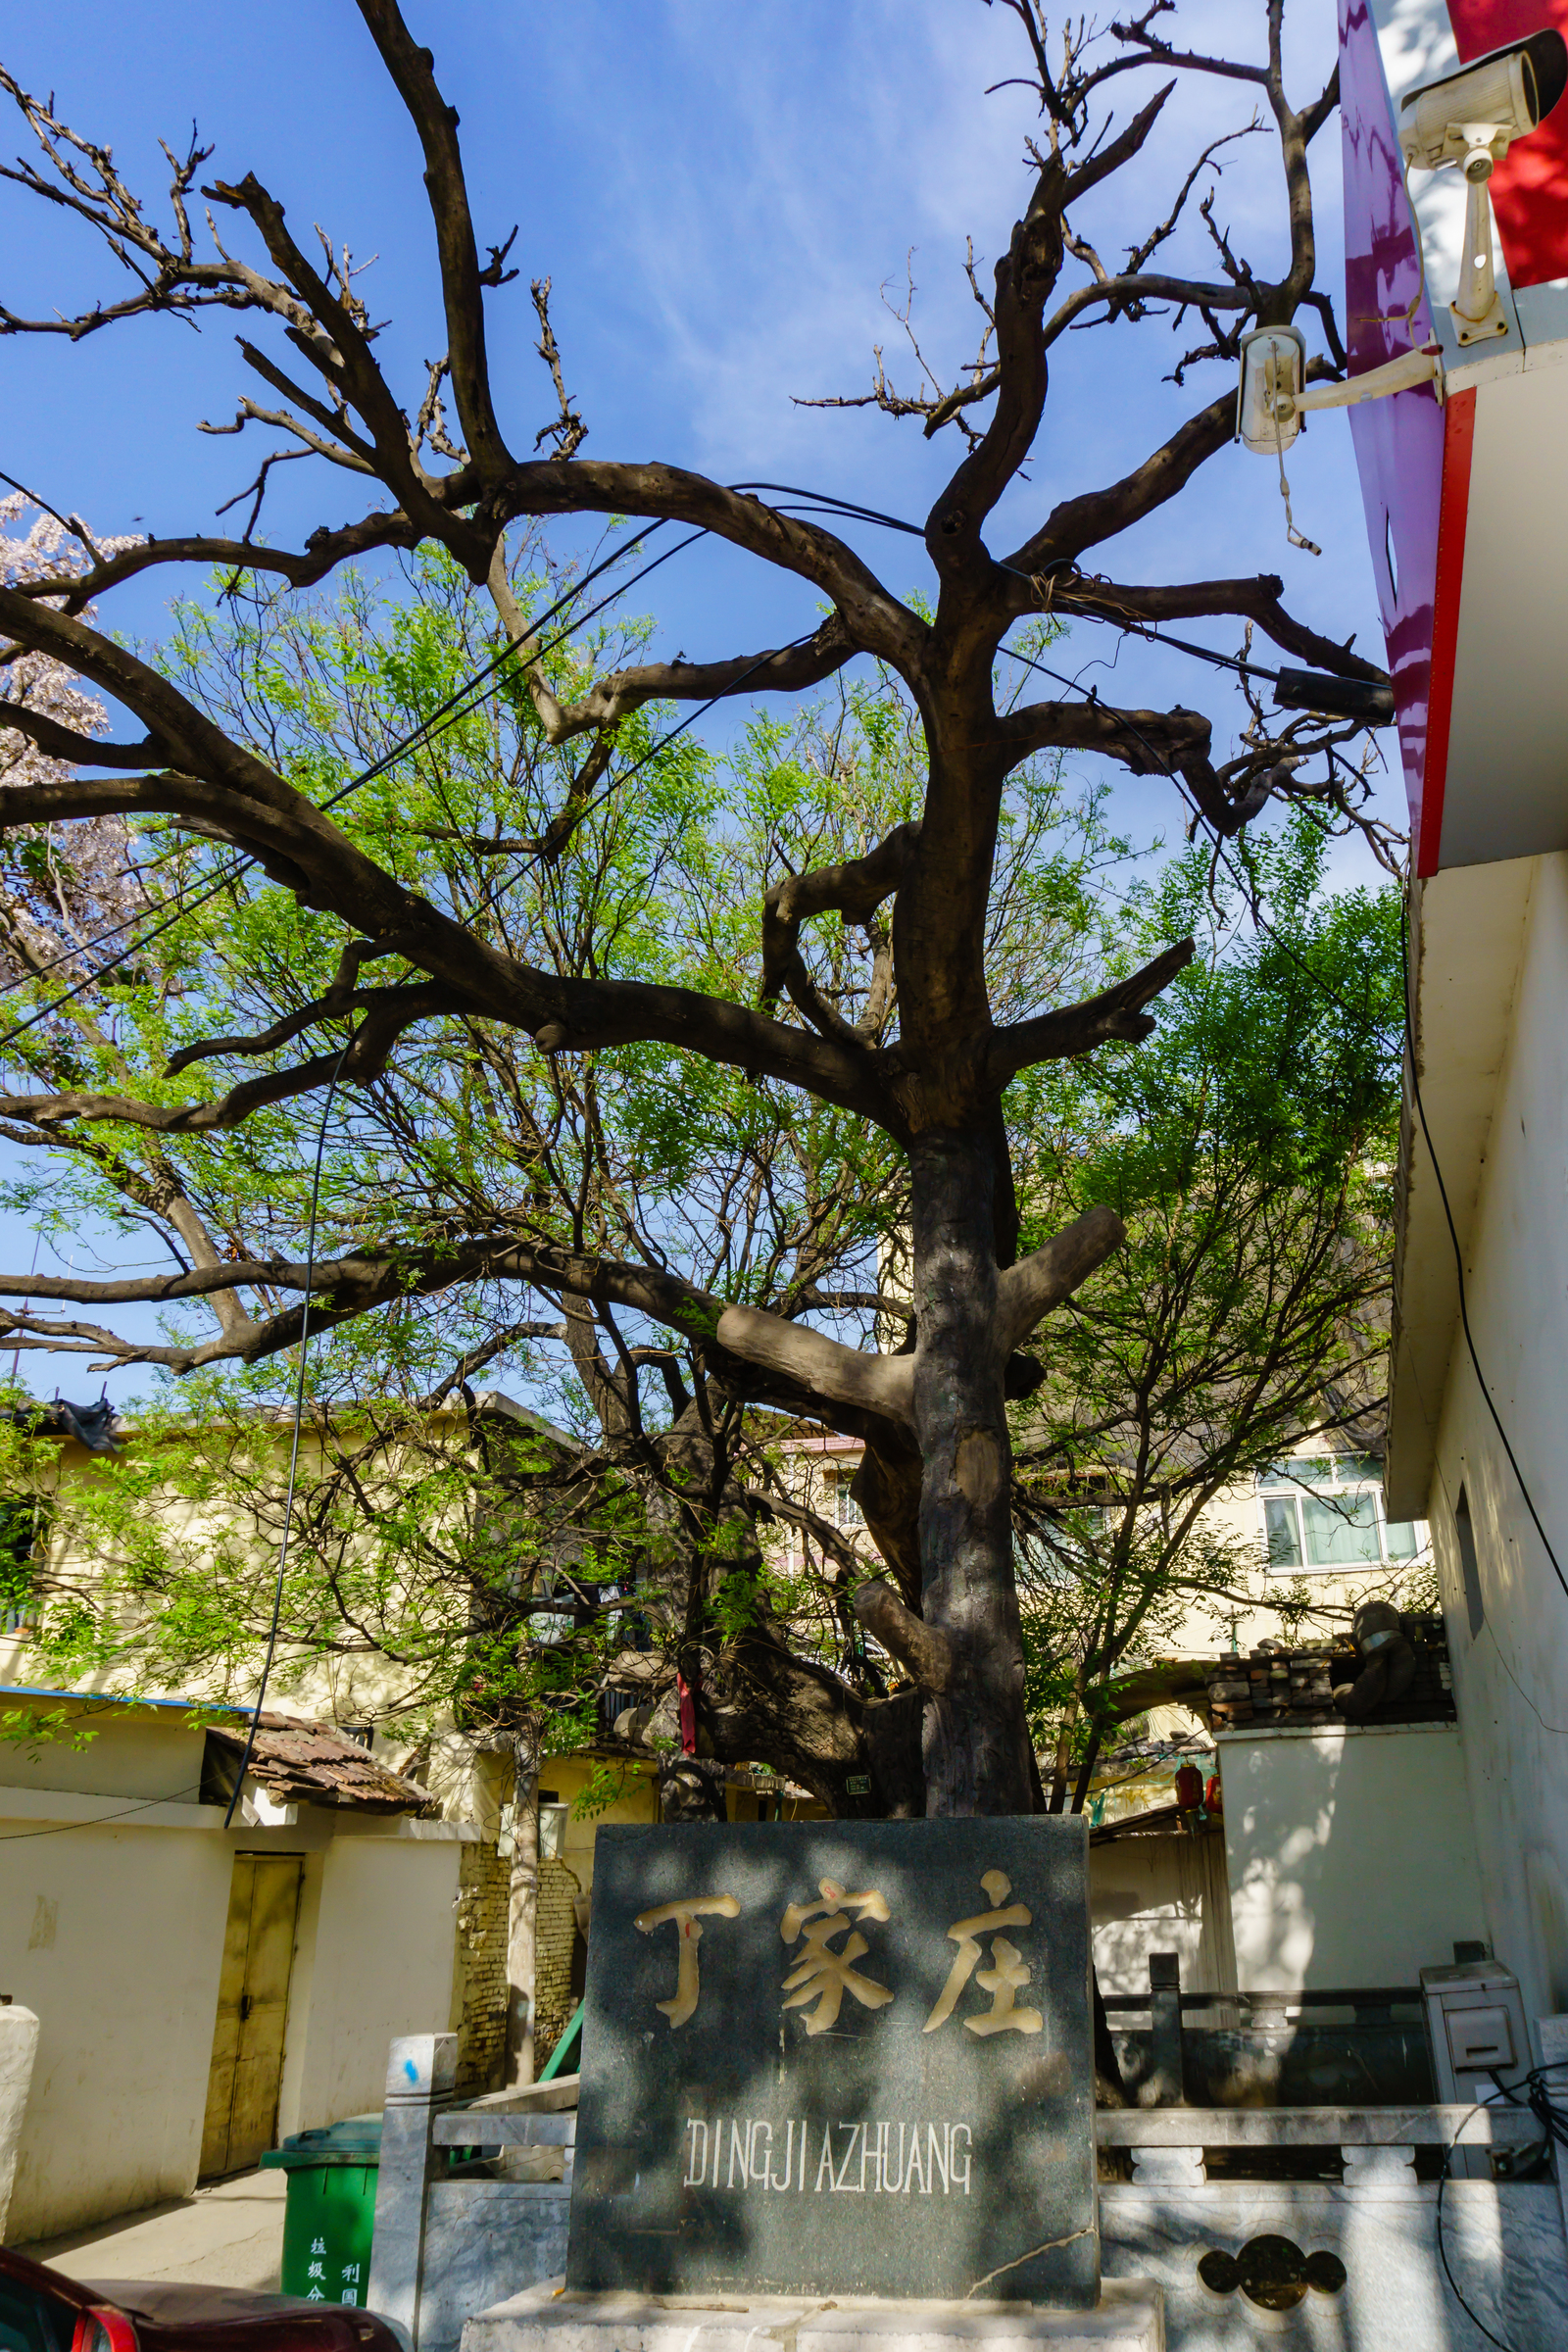
\includegraphics[keepaspectratio, height = 0.6\textheight]{dingjia/cunbei.jpg}
  \caption{丁家庄村碑}
  \label{fig:cunbei} % \raggedright \raggedright \small 2017年4月20日,丁家庄村口的村碑和百年老槐树。
\end{figure}
\clearpage


\dingphotoh{sanbadaji}{熙熙攘攘的三八大集}{2017年5月8日,丁家庄每逢农历三、八为大集。}{zuwu1}{北侧一处出租楼房外景}{2017年4月7日}

\dingphotov{guodao1}{一条街道}{2017年4月7日。}

\dingphotoh{guzhai}{城中村最为破败的一间自搭棚户}{2017年5月6日}{bizhezuwu}{笔
  者田野调查中租住的单间}{2017年4月25日,月租金240元,网络费30元,居住条件在
  城中村属于中等偏上。}

\dingphotov{chucangshi}{夫妻二人和他们一岁孩子所租住的储藏室}{2017年4月15日}

\dingphotov{cesuo1}{城中村中等水平的简易卫生间}{2017年3月31日,这类卫生间多为
  房东所建,常常加锁,只供其名下租客使用。}

\dingphotoh{yangguang}{阳光}{2017年4月26日,木制挂锁卫生间。}{lou1}{二楼房顶
  私搭简易板房}{2016年11月20日}

\dingphotov{shaoshui}{丁家庄村民常用的木柴铁皮桶炉}{2017年5月8日,丁家庄一些
  村民为节俭持家常用这种简易炉烧开水,火力弱,耗时长、烟雾较大。}

\dingphotoh{youeryuan}{幼儿园外墙与线缆}{2017年3月31日。}{wanshua}{玩耍的孩子
  们}{拍摄于2017年5月7日。}

\dingphotov{jiagai}{改造楼梯、层层加盖的一座楼房}{拍摄于2017年5月11日}

\dingphotoh{jiejing2}{街景}{2017年3月26日}{caishichang}{丁家庄综合市场中的一
  处菜摊}{2017年4月26日,年租金近9万,年耗塑料袋1万元左右。虽然是大棚内的开放
  式摊位,租金比综合市场中的活动板房小吃店还要高不少。}

\dingphotoh{caitandajie1}{城中村内一处简易搭建的菜摊}{2016年12月14日,城中村
  内一处菜摊,这里并无租金。内有被褥,卖菜大姐应当也睡在这里。}
{caitandajie2}{简易菜摊消失了}{2017年3月8日,许是抵不住严寒和微薄收入,卖菜大
  姐和她的摊位不见了,只有床垫。}

\dingphotoh{zhian}{墙上张贴的治安告示}{2017年3月31日。这里盗窃案件可能略高于
  济南市其他小区,但远未达到恶劣的程度。笔者数十次进出丁家庄,未曾见过街头吵
  架斗殴。}{diushi}{一位走丢的小孩暂在三轮车摊主的怀抱中睡着}{拍摄
  于2016年11月09日,小孩从综合市场误入城中村,寻不见家长大哭不止,后在三轮车
  饮食摊主怀中睡着,身上披着他人提供的大衣。}

\dingphotoh{hua1}{一处住户外侧的绿植与杂物}{2017年4月12日。}{yangtai}{一处阳台——花与衣}{2017年4月12日。}

\dingphotov{cbd}{丁家庄工业南路南区一户未拆住房的外墙}{2017年4月20日,丁家庄南区是第一批拆除的宅基地住房,当时已达成动迁20余户,只余3户尚未动迁。}

\pagestyle{fancy}
\chapter{城中村的简单概念}

所谓城中村者,城市和村居性质兼而有之:它往往位于城市中心或郊区,作为城市的一
部分,周边均具城市特征,自身却充斥着农村式的无序和自然,缺乏人工的总体规划,
各家各户的宅地界限比传统村庄混乱得多,基础设施(能源、通讯、供水、交通、安全、
卫生、医疗、文化等)薄弱,常生人口基本为农村户籍,土地制度仍为农村集体所有制
而非城市的全民所有制;作为农村,它的外来流动人口数量数倍,甚至数十倍于常住人
口,耕地被大量或完全占用,转为商业或住宅地产,耕地的这种性质转变使常住人口原
赖以生存的农业收入转为地产收入,并成为其收入的重要来源。

2016年《联合国人居三筹备委员会第三届会议政策文件10:住房政策》(文号A
/CONF.226/PC.3/23)对贫民窟词条所作的解释为:
\begin{quotation}
  自 2003 年起,联合国会员国商定将\textbf{贫民窟家庭}界定为生活在同一屋檐下,但缺乏
  以下五项条件中的一项或多项的一组个人:(a) 能得到经改善的饮水;(b) 用得上经
  改进的卫生设施;(c) 充足的居住面积-不过于拥挤;(d) 住宅的结构质量/持久
  性;(e) 土地保有权的保障。
\end{quotation}

我们通常所说的城中村可以认为是中国政府棚改文件中定义的“城市棚户区”,并且明
显属于联合国定义的城市贫民窟范畴。\cite{unandchina}


中国的城市贫民窟人口有多少呢?联合国人居署提供的往年数据如下:
% Please add the following required packages to your document preamble: % \usepackage{booktabs}
\begin{table}[!ht] \centering
\label{my-label}%
  \caption{1990-2014年中国城市贫民窟人口比例及数量}
  \capsource{联合国人居署旗舰报告《World Cites Report 2016》\cite{9789211327083}}
   \adjustbox{width=\linewidth}{%
    \begin{tabular}{l|l l l l l l}
      \toprule
      & 1990年 & 1995年 & 2000年 & 2005年 & 2010年 & 2014年 \\ \midrule
      城市中贫民窟人口的比例(\%) & 43.6 & 40.5 & 37.3 & 32.9 & 29.1 & 25.2 \\
      城市贫民窟人口的数量 & 1.316亿 & 1.514亿 & 1.691亿 & 1,835亿 & 1.806亿 & 1.911亿 \\ \bottomrule
    \end{tabular}%
  }
  \end{table}

  根据《国家新型城镇化规划(2014-2020年)》,我国预计“到2020年基本完成城市棚
  户区改造任务”。根据2018年第十三届全国人大一次会议政府报
  告\footnote{\url{http://www.gov.cn/gongbao/content/2018/content_5286356.htm}},
  “棚户区住房改造2600多万套,农村危房改造1700多万户,上亿人喜迁新居”。全国
  轰轰烈烈兴起的城中村改造跑步前进,新型城镇化取得了惊人成绩,这同时也标志着
  曾经遍布每个大中型城市的老式城中村的大量消亡,丁家庄城中村也在其中。先
  让我们看下曾经的丁家庄是什么样子吧。

  \chapter{济南市丁家庄城中村见闻散记}

  \section{背景介绍}

  济南市丁家庄,又名丁家村、丁家新村,据1992年5月1日所立村碑记载:
  \begin{quotation}
    明永乐年间(1403-1424)当地根据传说取村名“定妖庄”。后因此名不雅,故
    以“定”字谐音“丁”字改为丁家庄。
  \end{quotation}

  丁家庄隶属于山东省济南市姚家街道,曾是济南市一个较大且密集的城中村,
  在2000年前就已开始为外来务工人员提供住房等服务,共有村民宅基地(院落)
  近800户5000人,外来流动人口峰值大约可达30000人。丁家村城中改造是山东省棚改
  旧改的重点项目,于2017年年底基本完成房屋拆除工作,拆迁面积约为53万平方米,
  包括村民宅基地、公益性公共设施用地和经营性用地等,整体搬迁至奥体西路新建高
  层小区。

  \section{初见}

  笔者初入丁家庄时便因它表面的破败和杂乱而产生一种恐惧感。整个城中村
  除20余栋6层楼房以外,基本全是村民自建、层层加盖的三四层楼房,有的自建房已有
  些轻微倾斜,有的在房顶上再加装简易活动板房;各种样式的电线、网线、不明用途
  的线缆随意聚成一团团,与敞盖或无盖的配电箱、歪七扭八的电线杆纠结交织,这里
  似乎随时会演变为危房倒塌或大型火灾或现场。笔者倒是未听闻未见相关事故,或许
  是因户主租户有一套自发自治管理的办法。

  条条未经规划和硬化的水泥石板路路面也是蜿蜒曲折,纵横交错整个村落,笔者游历
  丁家庄数次之后才可不迷路。出租房基本都是单间,十几二十几户共用户主搭建的公
  共厕所,楼上住户冬天起夜时还要穿衣下楼,并不方便。村民们多是传统农民打扮,
  外来务工人员衣着也称不上光鲜亮丽。过往中国农村生活条件艰苦,重病患者、残障、
  丧失劳动能力的比例往往大于城市,而丁家庄这里的比例可能比传统农村还要高。笔
  者有次刚要走出丁家庄时碰见村口一位50岁左右的男子坐在轮椅上斜着头,面无表情、
  眼神空洞,对周围不管不问地在晒太阳,或许是偏瘫。未过几秒,迎面又走来一个怯
  生生的30岁左右的男子。他提着午饭低头走来,看见我时便将整个身子直接旋转180度,
  定在原地,用后背对着我,不敢和我有一瞥眼的接触。当我正要和他擦肩而过时,这
  位男子又朝无人那侧180度急速转身,继续前行,他应有视线恐惧症或社交恐惧症等精
  神疾病吧。不过有熟识的村民也向他热情问候。\improve{缺乏对居住人口的描写}

  未接触过城中村的人,初入丁家庄,很难不恐惧吧,毕竟这里像是随时随地会发生刑
  事案件一样。然而,这确实多虑了。房东们多会查看并登记租户身份信息,考察租户
  人品性格,周边人群间的关系也比高楼大厦上来得亲密一些。一只只小小的、防君子
  不防小人的普通挂锁足以保证财物安全。不知怎的,当我在那不足10平的单间里住宿
  时,却比在现代小区高楼上居住更加平静和坦然一些。

  \section{黑夜与清晨}

  丁家庄城中村的夜总比周边来的更早些。

  街道路灯不多,住户多使用散发着黄色光晕的白炽灯。晚上八九点钟,灯光和墙面组
  成的黄色主色调混合着个别店铺的七彩霓虹灯光闪耀在城中村里,叮叮当当的做饭声
  时常响起,笔者还见过住处一楼楼廊里一位不足10岁的小男孩独立炒菜做饭,归来的
  叔叔阿姨们在路过时对他不吝赞叹。

  深夜,村外尚有较晚收摊的小吃车、大排档、夏天24小时营业的烧烤店、为深夜食客
  们服务的小零售店、长明的路灯和过往的车辆。村里却是另一片景象,这里更黑更静。
  晚10点左右还能偶尔听见晚归人家的锅碗瓢盆交响曲,11点左右整个村子便一下子寂
  静起来,水泥石板路上鲜有路人。偶在没有路灯照耀的环卫点,有一位老人在几个垃圾箱
  中翻找可再利用或可卖的杂物。

  这里的早晨也比周边来的更早些,6、7点钟各处雄鸡打鸣,各家各样的声音均透过不
  隔音的墙壁和窗户传到家家户户,问候声、寒暄声也此起彼伏。孩子、送孩子上学的
  家长、上班族一下子散布各处,城中村在这个时间已经开始繁忙起来。

  \section{医疗保健和社会保障}

  因笔者能力有限、怠惰和调查时间选择上的问题,被调查人群多为中老年人并且数量
  很少。虽然存在这种样本偏差导致不能推导出一般性的结论,但笔者认为可以提下自
  己直观和经验感受:不管是流动人口还是常住人口,他们身高较之周边明显偏矮,心
  脑疾病较多,也有被调查人家庭两代人中均患重大疾病的事例。《中国心血管病报
  告2017》中开篇有提“我国居民心血管病(CVD)危险因素普遍暴露,呈现在低龄化、低
  收入群体中快速增长及个体聚集趋势。”,贫穷始终是种顽疾,甚至是绝症。

  根据“丁家庄环境卫生管理公示牌”,丁家庄有保洁人员21人,保洁面积4万平方米。
  据本次调查,济南市环保局贯彻执行八小时工作制,并为保洁人员缴纳三险。所聘用
  保洁人员多为丁家庄居住人口,每月到手收入在1600元左右。济南市环保局在劳动保
  障上的表现出乎笔者意料,在此点赞。另外,有一例保洁员工伤纠纷,当事人为外地
  来济60多岁老人,因是否算工伤与环保局有分歧,环保局领导也曾亲切慰问。虽然当
  时问题并没有解决,但当事人对国家和政府仍表示“非常满意”,没有任何意见。

  丁家庄老年村民大多没有缴纳任何形式的养老保险,包括新型农村社会养老保险(新
  农保),也不了解具体政策。满60岁老人由村委每月补助600元左右。丁家庄大部份村
  民所能缴纳的社保只有新型农村合作医疗(新农合),有每年缴纳100元和300元两个
  档次。新农合在丁家庄村民重大疾病治疗上发挥了极其重要和显著的作用,常可报
  销60\% 多的费用。

  \section{何不食肉糜}

  虽然丁家庄北侧就是一个较大的综合市场,供周边几个社区的居民采购农副产品,生
  意兴隆但年租金昂贵,大菜摊租金约9万元/年。城中村里仍有些蔬果摊子长期固定在
  街道一角,它们铺设在水泥道路或机动三轮车上;还有些定期定时流动叫卖的轻型贩
  菜货车。城中村蔬果摊主要面向城中村内中老年居民,无需承担任何租金,多供应次
  一级的菜品并且价格低廉,但销售额和利润远不能于综合市场相比。 (可参
  考\cref{fig:caishichang}, \cref{fig:caitandajie1},
  \cref{fig:caitandajie2}。)

  这里我们来谈一个架设在机动三轮车上的水果摊主吧,笔者将其隐去名讳,代称为刘
  哥吧。即使在城中村,刘哥家的居住环境可能仍是最为糟糕的,他一家三代住在一
  个200多元月租的单间中。他的立业史,也是每一步都恰被时代所驱赶和压迫的悲剧史。
  他做过走街串巷流动叫卖的小贩,被驱逐淘汰;又做过居民小区外较固定的摊贩,被
  驱逐淘汰;又做过丁家庄综合市场外路边摆摊的摊贩,相较综合市场的高额租金,路
  边摊所需费用便宜太多,同样也是被驱逐淘汰;最后刘哥成为了城中村内一个机动三
  轮车上的瓜果小贩。2017年丁家庄已被夷为平地,刘哥不知又将以何种方式去拖家带
  口继续书写他自己的立业史……

  夏季的一天,笔者碰到他十岁左右的儿子从自家中捧来几片薄切的西瓜给他吃,可
  他明明就是卖瓜的呀。

  笔者无论如何也没有想到,当笔者向一些人说起丁家庄综合市场和城中村菜摊的区别
  时,有些人会指责刘哥不努力不争气,质疑他为何不早在综合市场租摊位(高租金)
  以求得良好收益。一个一家三代居住在城中村破败单间的外来人,如何去承担每年数
  万的租金啊。我记得90年代初当我还是个小孩时,并没有铺天盖地地听到“成
  功”“成功人士”这类说法,对于贫穷者多半是怜悯其境遇不佳。今时简单用资本结
  果作为个人能力的衡量标准,从而一叶障目时,我们都将成为那个呆傻可笑的晋惠
  帝,“百姓无粟米充饥,何不食肉糜?”


  \section{过往的宅田基地之殇}

  % “社会空间” 概念。他把社会空间理解为 “空间的实践”、 “空间的表象” 和
  % “具象的% 空间”的三位一体。也就是说,空间不是一个抽象的存在,而是自然的、精神的和社会的三位% 一体,这个一元的整体性的社会空间既是逻辑-认识论的空间,同时也是社会实践的空间和亲身% 经历包括感觉想象的空间。通过这个包含着诸多规定和关系的社会空间概念, “社会空间” % 概念。他把社会空间理解为 “空间的实践”、 “空间的表象” 和 “具象的空间”的三位% 一体。也就是说,空间不是一个抽象的存在,而是自然的、精神的和社会的三位一体,这个一元% 的整体性的社会空间既是逻辑-认识论的空间,同时也是社会实践的空间和亲身经历包括感觉% 想象的空间。通过这个包含着诸多规定和关系的社会空间概念,

  % 列斐伏尔强调,三元分析的三个方面是既相互独立又相互作用的,三重要素中每一个方面都可% 以也应该在与其他两个方面中的任意一个的相互关系中得到理解。并且任何一个要素对于其% 他两个都不具有绝对的优先地位。

  % 社会空间是 “空间的实践” (spatial practice)、 “空间的表象”(representations
  % of % space)和 “具象的空间” (representational spaces)的三位一体。社会空间的生产可以从% 这三重概念的辩证运动中得到理解。相应的,如果我们从身体出发理解社会空间,这三重图式% 又可以表达为 “感知的” (the perceived)、“概念的”(the conceived)和 “经验% 的”(the lived)。


  % “空间的实践”
  % 包括生产和再生产,以及构成每一社会的典型的具体场所和空间化% 的位置。一个社会的空间的实践通过保证连续性和凝聚力,生产并隐藏这一社会的空% 间。

  % “空间的表象” 是概念化的空间。

  % “具象的空间” 既是作为 “居住者”、“使用者” 或 “占用者” 的人们生活于其中的空% 间,包括房屋、教堂、广场等;也是一些艺术家、哲学家、作家们所描述但又渴望不仅% 仅是描述的空间。因此,一方面,具象的空间与人的真实的生活经验相连,与空间的表

  在中国传统小农经济的农村中,往往以家庭为基本单位,主要活动范围局限在村内,
  生产集中在自家规模极为有限的耕田或从事简单手工业、半加工业的家中,生活集中
  在自家住宅与村内公共空间。田区和住宅区常常分隔明显,呈大块状分布,同一大块
  内常是多家彼此有联结的田地或住宅,其中相联两家之间的田地多用沟、垄、界石作
  为田界,住宅多用共用的一面墙壁或距离极近的两面墙壁作为宅界。

  多数人的社会空间长期固定、聚合、封闭在居住村,物质和社会资源有限,生产生活
  单调贫乏,村民之间联系频繁,信息传播速度快,这种情况下发生的利益冲突常常尖
  锐持久、难以调和,田界和宅界作为最重要的家庭产权,具有相当刚性。

  在实践和具体的社会空间中,这一刚性界限却又常常变动并受到侵蚀。它本身包含农
  村中通风、采光、日照、排水、通道等难以界定的方面,另外在国家和政府层面来说,
  又有历史遗留、立法不健全、执法成本高等问题;在村民来说,则有历史遗留、普遍
  违规超额占用、法律维权成本高、法制观念不强、宗族势力等问题。

  如果氏族大家庭或直系小家庭被其他大小家庭侵犯界限而未采取有效措施,则不单是
  家庭经济效益,连带个人和家庭的自我认同、社会地位也将受到严重的负面影响。这
  也使宅、田基地矛盾相当尖锐频发,家庭中的强壮男子往往被赋予保卫甚至扩张这一
  刚性界限的责任。过往中国对家庭伦理的重视,甚至重男轻女等现象,也多由此建立
  起来。

  在笔者对丁家庄的走访过程中,也曾碰到宅基地纠纷当事人商姐说起一例二十多年前
  的惨剧:两家因新修墙壁越界而产生的宅基地矛盾步步升级,致使受到屈辱的商姐丈
  夫自杀。商姐带领家人将邻居群殴至半死,法院支持了邻居的索赔诉求,但商家一家
  并未履行法院判决,于是肇事方二十余年不允许商姐家开发自家一块空地。

  丈夫自杀后,商姐带着两个儿子独立生活,其中小儿子当年不到两岁。她抓住了空间
  转化的时机,是90年代丁家庄第一批建立租屋的人。丁家庄拆迁前她的租屋总面积已
  经超过1500余平,出租房屋超过50户,月入过万,在丁家庄这也是了不起的成就。她
  的两个儿子也争气,可给她带去一些宽慰,只是长年的劳苦使其腿病明显,面态老相,
  但商姐勤劳不改,晚上仍会去丁家庄综合市场进行清洁工作,以换取一些额外的微薄
  报酬。总是风风火火、穿着男式西装、一瘸一拐地支撑起整个家庭的商姐啊……

  当商姐以维权为理由倾诉她的故事时,笔者一再说明我这个自发小项目不能给其带来
  任何改变,也难以根据她的一家之言去支持她时,她对笔者的中立态度表示认可,最
  后甚至还埋怨起她的家庭当年为什么不让一下那寸土的界限,即使再让更多些也不要
  紧啊……

  诉说过程中,笔者渐感商姐并非真要维权,并非还存那样的恨意。她曾说要带笔者去
  看那块因久被搁置而自然成为停车场的空地,笔者当时就感觉可能不需要了,事实上
  也是如此,事后我为求证自己想法向她两三次询问时间安排时,她果然都借故推脱,
  并刻意回避我。

  她真正想要的其实只不过是一场没有利害关系的倾诉……倾诉完之后当事人产生了羞
  愧感,不敢面对被倾诉人;而所谓仇恨早已经在时空的变换中变成了一介难以抹去的
  难看疮疤。

  随着丁家庄旧村改造的完成,丁家庄人将进入新的、现代化的城市空间,城市空间中
  的界限更为明显也易维权,原本农村中典型的宅基地矛盾将很少存在,希望两家日
  后能够相忘于江湖,也同样希望人们彼此能够多一些理解,多给一些倾诉的空间,以
  使悲剧不再那么多,那么难以承受……



  % 丁家庄城中村是一个充斥着盎然生机、孕育着诸多可能的城中村。它是许多人实现梦想的起% 步点或中转站,也展开怀抱接纳了各方边缘人群,诸多住户之间较为和谐。它也远未成为一% 个堕落之处,这里并非治安恶化严重,


  % \section{失败的丁家庄城中村社会学调查}

  % 笔者起初准备以定量研究方法结合定性研究方法对丁家庄作一个较为全面的社会调查。其中定量方面,仿照ISSP\footnote{The International Social Survey Programme,国际社会调查方案}和中国的CGSS\footnote{Chinese General Social Survey,中国综合社会调查,于2007年加入ISSP。}问卷作一个针对丁家庄城中村的调查问卷,定性研究初步决定采用Phil Francis Carspecken的批判定性研究框架。

  % 之后笔者又十几次进入丁家庄,也曾在丁家庄居住做过1个月进行田野调查,但因自身怠惰和三心二意使本次调查大失败,不过以下几点心得或许有益于类似社会调查的开展,在此分享给读者:
  % \begin{enumerate}

  % \item 定性研究一般要求记录谈话,录音常是记录谈话的主要方式。扎根理论和Carspecken的定性框架必须建立在大量谈话资料的多次整理上。但丁家庄人均谈录音色变,拒绝录音。这种拒绝主因是被调查人在敏感性的事件上害怕录音成为某种对自己不利的证据。

  % \item 城中村人员组成和住房结构的复杂,使针对整体的概率抽样问卷调查非常困难。实际上笔者认为,只有具有政府背景的组织或机构大力支持、推动才能完成类似复杂区域定量研究的概率抽样。

  % \item 笔者采用了非概率的随机街头访问方式发放调查问卷,这使调查结果可能产生无效的、完全不具代表性的样本。并且即使如此,问卷回收率仍然极低,只能勉强算是10\%,使定量分析成为不可能。

  % \item 利益敏感问题信度不高。除笔者本人能力拙劣外,也有现实客观。例如针对房东的调查中,房东往往隐瞒和减少实际出租房屋间数以及出租收入,可从被调查房东所处房子建筑外观、体积以及丁家庄出租房的平均面积和收入得出这一信度不高的结论;针对所有人的收入问题也存信度问题,再三询问或试探所得出的收入结论最高浮动为1000多元人民币。调查问卷中针对村委和拆迁方案的满意程度采用了5级李克特量表,但被调查人极端选择较多,情绪化明显,个人利益最大化主导的倾向明显。

  % \item 半数以上房东有对上级政府机构的强烈诉求,这也是他们对社会调查人最大的期望。本次调查为笔者个人自发,没有任何组织机构背景,也一再向被调查人言明本人所写报告预计不会产生任何一点社会影响力,无法满足房东这种诉求。除此之外,社会学可以采取小额金钱奖励的方式来增加被调查人积极性,但笔者着实囊中羞涩,无法采用这种方式。

  % \item 租房人对本次社会调查表现出严重的整体冷漠,可以认为这是一种社会排斥。关于这方面内容,笔者放在之后章节再详细论述。小额金钱奖励应可以有效提高租房人积极性,但未实施,原因同上。

  % \item 最主要原因仍是笔者个人社会调查能力的欠缺,和态度的不端正。笔者接触社会学是在丁家庄摄影项目受阻之后从零开始,在社会学意义上的与人交往也存各种缺陷。最主要的还是态度,三心二意、半途而废,甚至因屡次消沉而遗失了几份已经回收的完整调查问卷。

  % \end{enumerate}

  % 本次调查过程中,笔者听闻有两位女士几乎同期在丁家庄城中村进行社会问卷调查,并对问卷完成者提供每人50元奖励,效果不错。笔者估计是具有政府背景的组织机构,如大学在做这份工作。希望我国能够在当前基础上进一步普及社会学调查相关知识,增加社会学调查项目,并保证社会学调查的中立性及公信度,同时也希望调查者能够坚守信度和效度问题。

  % 下一节笔者将介绍在丁家庄中的所见所闻所感。



\part{人文}
\chapter{当代艺术}

\section{当代艺术的概念}

什么是当代艺术,它具体起源于何时,主要表现是什么?像艺术的概念一样并没有一个
确定而公认的答案。在众说纷纭的“当代艺术”概念阐述中,往往也存在着观念艺术、
后现代艺术、当代艺术这三者之间界限不明、混淆不清或者顾此失彼的问题。

在《詹森艺术史》中,只介绍了比较细分的观念艺术和后现代艺术等,没有单独提及当
代艺术 。但笔者认为《詹森艺术史》后现代时代一章中关于艺术哲学理论发展和影
响的阐释较为精准到位和克制。

\begin{quotation}
  20世纪80年代以来,艺术界关注的艺术风格通常被称为后现代艺术(Postmodern
  art)。60年代中期,欧洲文学评论界确定了“后现代”这一术语的含义,并首先在文
  学领域使用;这个圈子的核心人物是法国哲学家雅克·德里达(Jacques
  Derrida,1930-2004年),其理论也被称为“解构主
  义”(Deconstructionism)或“后结构主义”(Post-Structuralism)。\medskip

  50年代和60年代期间,罗伯特·劳申伯格、安迪·沃霍尔和罗伊·利希滕斯坦都对这
  一问题很感兴趣。虽然后现代主义在视觉艺术领域的灵感来源就是这个时期,但艺术
  界真正自觉进入新时代的情况直至70年代晚期才出
  现。\pagescite[][1077]{9787510048623}\medskip

  他们还受到另一位法国后现代哲学家或后解构主义哲学家让·鲍德里亚(Jean
  Baudrillard,1929-2007年)的影响,后者的拟像(simulacrum)理论影响尤为重
  大。…… 超级现实,通过包含电影、电视在内的大众媒体,美国人创造了一个虚假、
  完美、永恒的世界,仿佛比现实本身更加“真
  实”……\pagescite[][1094]{9787510048623}
\end{quotation}

国内王端廷在《西方现代、后现代和当代艺术的分期与区别》一文中,将后现代艺术风
格断代为1979-1989年,当代艺术风格断代为1989年至今。并提出“对审美的回归是当代
艺术的总趋势”,“什么都是艺术”,“人人都是艺术家”的观点已经过时。但是我们
看到,王瑞廷文中所说当代艺术的“普世主义”仍未脱出后现代理论语境,仍是用后现
代理论作为指导。\cite{wangduanting}

周计武在《什么是当代艺术》一文中,认同阿瑟·丹托和汉斯·贝尔廷的看法,将过往
被叙事逻辑支配的时期被称为“艺术的时代”,即艺术在其中具有明确的历史方向和历
史意义的时代。它开端于文艺复兴时期,终结于20世纪60年代,被如今没有大师叙事的
后历史时代所取代。在丹托看来,“后现代”一词过于暖昧,既可指现代之后的艺术,也可
指现代艺术体系内的自我批判。因此,丹托主张用“当代艺术”替代“后现代艺术”一
词。\cite{whatsart}但令人奇怪的是,周计武为何将79年的“星星”美展和“85美术新
潮”定为当代艺术,看其表达形式和内容、意义,笔者认为,这应当还是算作现代艺
术。

笔者认为,周计武所提到的内容是当代中国最为广泛接受的“当代艺术”概念——来源
于丹托“艺术终结”论的观点。
\begin{quotation}
  “艺术死亡”、“艺术史结束”、“人人都是艺术家” 的呼声,在当代欧美美学界和
  艺术界越来越高 ,对中国本土的美学和艺术也开始产生重要影响。这些 “空洞口号”
  既非艺术家也非纯美学家所创,而是肇始于当代美国分析哲学家阿瑟·丹托 (Arthur
  C.Danto)的 “艺术终结” (the End of Art) 的宣称。\cite{boduoyishu}
\end{quotation}

如贡布里希所说,对艺术风格整齐的年代划分只是艺术史家或艺术史爱好者所喜欢用的
方法,不可能有一个绝对正确时间段的当代艺术划分,但上述所提及的当代艺术概念其
实是求同存异的,尤其是在后现代理论对他们的影响方面。

结合实际,在当前国内当代艺术作品鉴赏中,抽象的、底层的理论方面,我们看到策展
人、艺术家自称的铺天盖地的“解构”、“拆解”、“碎片化”以及德里达、利奥塔、
福柯、鲍德里亚等人的后结构、后现代理论引用和更早提出“反艺术”的阿多尔诺的理
论。

在通俗具体的当代艺术解释上,国人则喜欢用“反艺术”,“人人都是艺术家”,“不
止审美也审丑”,“重要的是理念,而非形式”“一切皆可”等丹托的“艺术终结
论”观点。其实就丹托文章内容和参考文献来看,丹托“艺术终结论”的提出应该也是
受德里达之前提出的文学、历史等终结论的影响。

本文将从丹托“艺术终结论”和后现代理论两个方面来考察当代艺术。

\section{后现代理论起源和发展} \unsure[inline]{这一节先留着,对理论不感兴趣的人可以不看。不排除以后将当代艺术一节归入后现代章节下,届时本节将归入后现代。}


对于后现代理论从何时开始发展,没有一个唯一的答案。较多人接受后现代发起于20世
纪中后期,道格拉斯·凯尔纳和斯蒂文·贝斯特认为真正提出一个新的后现代纪元这一
观点的是法国的鲍德里亚和利奥塔。

法国最先宣扬历史出现后现代断裂受几个方面影响:法国二战后出现的迅猛的现代化进
程,农业为基础的社会变成了主要以城市和工业为基础的社会,资本主义带来高速发展
的生产力和科学技术;五六十年代哲学和社会理论所取得的令人振奋的进步,马克思主
义、存在主义、现象学被语言学倾向的结构主义和拉康精神分析所代替;1968年法国五
月风暴所引发的强烈的决裂感,许多人开始反思马克思主义,尤其是法共所讲的马克思
主义是否过于教条和狭隘甚至是压迫性的,不能从理论上说明当代社会及其多样化的权
利样式,并且批判了把知识当成获取权力和统治工具的做法,也批判了自由主义制度在
解决民众不满情绪方面的无能。

结构主义进一步发展为后结构主义(解构主义)。后结构主义把能指\footnote{语言符号中
  的视听acoustic visual成份,今天被解释为可被听、闻、触、视、尝到的物质形式}放在
比所指\footnote{语言符号中的概念性成分}更重要的位置上,以此来表明语言的动态生产性
和意义的不稳定性,表明他们同意义的再现图式的决裂。他们认为能指仅仅是无休止的指意
(signification)过程中的一个瞬间。在这个过程中,意义仅仅是在所指的无限的、模棱两
可的游戏中生成的。代表人物德里达则成为后来一些后现代文学、艺术风格的理论建基者。

后结构主义逐步迈向多种多样的后现代理论。本文的主旨不在于具体阐述这些理论,而
是在于当代艺术批判,在此略过不表。

有意思的是,福柯、鲍德里亚均参加过法国共产党,并于50年代初退出。德里达则可以
算是个修正的后马克思主义者,而利奥塔也曾是马克思主义者,后来成为了有所背弃的
后马克思主义者。

\section{丹托的艺术终结论}

\subsection{丹托艺术终结论概览}

丹托的“艺术终结”并不是字面意思上的不再有艺术了,丹托想表达的是以往叙事的艺
术史已经终结,被如今没有大师叙事的后历史时代所取代。“一个没有历史方向、历史
意义和叙事导向的艺术”。

丹托认为,“艺术哲学史就是哲学压抑、剥夺艺术的历史。这与尼采的观点不谋而
合。”\cite{dantuozhenduan}这一哲学压抑艺术的历史向前可追溯至柏拉图的艺术模仿论,
在近代20世纪来看的话,则是:

\begin{quotation}

  请想想我们世纪令人眼花缭乱的一连串艺术,如野兽派、种种立体主义的表现、未来
  主义、漩涡主义、同步主义、抽象主义、达达派、表现主义、抽象表现主义、波普艺
  术、欧普(光效应)艺术、极简主义、后极简主义、观念主义、照相写实主义、新表
  现主义。(他们的寿命长则两三年,短则一个半月,且是“令人烦恼的艺
  术”。)……艺术的命令其实就是历史的命令——创造一个艺术史时期吧!——而成
  功就在于制造一种公认的新事物中。

  每个时期需要相当数量的相当复杂的理论,以便也能在艺术层面上处理时常是很微小
  的对象。面对历史定位与理论解放的深刻相互作用,对感情和表现的呼吁似乎越来越
  没说服力了。即使在今天,我们几乎也不明白立体主义几乎是怎么回事,但我确信在
  布拉克和毕加索宣布他们对吉他惊人一致的感情之后还有许多值得玩味的东
  西。\pagescite[][122]{7214029774}

  这些前不久的作品显示了另一种特色,那就是对象接近于零(前文提出的作品中在艺
  术层面上处理时常是很微小的对象),而其理论却接近于无限,因此一切实际上只是
  理论,艺术在对于自身纯粹思考的耀眼光芒中蒸发掉了,留存下来的,仿佛只是作为
  它自身理论意识对象的东西。\pagescite[][126]{7214029774}

  事实上,当艺术认识到一件艺术品不一定要成为某种特定的方式时,当艺术终结时,这
  种叙事就终结了。……追求哲学认同的艺术史结束了。艺术的价值就在于它允诺的自
  由:一种摆脱惨淡的人生境遇和冷酷的生活秩序的自由,一种自律的、审美的、不食
  人间烟火的“自由”。……在丹托看来,这种把美的艺术与生活分离开的“分类的权
  力就是统治的权力,而这些类似的审美状态(艺术哲学理论家的审美观)应被视为对
  双方感到的隐藏危险做出的反应,它本质上是政治性的。”\cite{dantuozhenduan}

\end{quotation}

丹托认为过往压抑或剥夺艺术权力的艺术哲学史模式被颠覆或“终结”,取而代之的是
一种新的“一切皆可、一切皆得为艺术”的“后历史”新艺术哲学。当代艺术来临了!

\subsection{丹托艺术终结论批判}

\begin{quotation}

  如果一切皆可,那恰恰成了一切皆不可……没有真理的断言,就没有激情,一切皆可,彼
  此彼此,就将导致相对主义、犬儒主义与虚无主义。但是丹托似乎高兴地宣告这一时代
  的来临,却不认为这足一种危机的症状。\cite{fuwendantuo}

  类似“一切都能成为艺术品”、“每个人都是艺术家”的口号,成为新的教条。这种
  深层结构上的复数主义,一方面,满足了大众对意义的追求,颠覆了现代主义叙事的
  精英倾向;另一方面,丧失了历史的意义和方向,暗合了新型中产阶级的意识形态要
  求。在某种程度上,它终结了不断进步的艺术史叙事。\cite{dantuozhenduan}
\end{quotation}

丹托的理论中,似乎是将艺术置于一个相当超然的位置之上,艺术在这里与政治、经济、
科技、生活等彻底分割开来,单独提前步入了丹托所说的“马克思的乌托邦社会——没
有界限的,绝对自由的后历史精神社会”。这怎么可能呢?!这简直是一个哲学门外汉
及现实门外汉的想象!在时间上和话语上,丹托应当是从德里达那里看到并拓展了“终
结”。但丹托的理论中却完全没有后现代理论中对现代性的批判成分,号称继承了尼采
的多元主义、反理论压迫、重酒神精神的生命哲学,最终却又完全背离了尼采,成为空
洞的,毫无生机与反抗精神的虚无。笔者甚至认为,丹托完全不了解后现代理论,只是
肤浅借用。

同时,丹托反艺术界中狭隘审美和理论的美好愿望非但没有实现,反而使艺术界的权力
上升至艺术历史中前所未有的高度,使艺术彻底抛离了大众并成为权力手中的玩物。如
果说过往的艺术霸权是通过关于审美和历史等方面的理论来实现的,如今的霸权则不需
要任何理论就可以实现。说你行你就行,说你不行就不行!

\section{结合后现代理论对当代艺术的批判}

当代艺术常有固定的范例和形式,这些范例和形式常被机械式地复制,创新为复制让路,
崇高为平庸让路,一切为艺术界让路,艺术界则为资本和权威让路。

% \begin{itemize}[noitemsep] %
\begin{itemize}

\item 日常中随处可见的俗物,简单直露到可怕的类波普艺术展示。大圣啊,快收了神通吧。
  朱熹和王阳明的“格物致知”,早在几百年前就吊打你们了。

\item 无人能懂的抽象,或者乱涂乱抹,层出不穷的棉花、各种材质的线和金属扭曲缠绕的
  非具象,或者用当代艺术说法——当代艺术想赋予我们的,正是人人都可以有自己的
  理解。虽然人人都是艺术家,而如果想对这种抽象进行“权威”解读并得到承认却需
  要依顺作者和权威人士的语言文字。

\item 带血伤口、血盆大口、超大眼珠、流出或散落的人体器官……还有对生命伦理的蔑视,
  劈成两半的动物,动物的头、器官和血。在80年代以前的纪实摄影师中,尤其是战地
  纪实摄影师,都极少去直接拍摄惨烈战场上的死尸、伤口和鲜血,这被认为是以猎奇、
  刺激、低俗的手法吸引观众,而将对战争和生命的反思置于二线。

\item 艳俗低俗的女性、男性裸体。人在此处往往只是充当物欲或者猎奇点。后现代理论中
  的微观欲望政治就“欲望在其本质上是革命性的”进行了扩展讨论并寄予厚望,希望
  能借解放自人类诞生之日起就有并伴随每人一生,促动人类社会发展变动的欲望、形
  成新的欲望方式来突破现代性的辖域。但在当代艺术、后现代艺术中,肉体往往只是
  肉欲的、物化的或者空洞的,这类艺术欲望毫无解放的张力,反被现代性彻底的役使
  所用。

\item 空洞乏味的行为艺术。阿布拉莫维奇2010年的《艺术家在现场》与男友乌雷的“偶然
  相遇”是其最为人所知的行为艺术作品,常令富有文艺或憧憬爱情的男女们感动,笔者只
  想说,来,干了这杯鸡汤!这鸡汤便是浓缩的艺术呵!噢,听说后来乌雷认为版权费给的
  太少,对阿布拉莫维奇发起了诉讼,至于诉讼结果如何,笔者无意关注。

\item 直接空洞的房间,或黑或白或兼而有之,可加一两句话,再配上几盏闪亮的灯那自然是最好不过。保守估计全世界有上千件这样形式的作品。“重要的是艺术家提出的观念,至于形式是什么并不重要”。何苦去看这些不成形的东西呢?经典文史哲哪个不提出观念,哪个不比你论述的更有感情、强度、深度……

\item 对中国国家政治、文化符号进行刻意的挑衅、抹黑,以此来获取一些西方不明真相群众或反华势力的“关怀”,其中关于天安门的“当代艺术”是重灾区。出奇的是,这一点被相当多的中国当代艺术家们前赴后继、乐此不疲地复制,还常能在国外各大小比赛中获奖。就这点来说,中西方的当代艺术界同样是令人失望的,他们只是以所谓反中国霸权体制的名头去投靠西方霸权体制而已。当代艺术的反政治是个天大的笑话。

\item 构成作品的单位元素数量众多,或作品面积、体积庞大,或超大场景,或耗费极大。

\item 被禁锢或污损的宗教文化符号,如笼中之佛,断头菩萨等。

\end{itemize}


丹托“艺术终结论”中,艺术界制度消失,但如本文上一节所说,艺术界的权力从未如此强大过。当代艺术所标榜的表达观念往往要被如前所述的出位、猎奇、空洞的形式所遮蔽。如果是还未出名的当代艺术家,除作品外还需要向“有关部门”递交artist statement(艺术家自述);成名的艺术家在拿出作品后常要备上访谈录、演讲或者其他艺术家的理解说明;艺术家们彼此写文、演讲,彼此歌功颂德,花花轿子人抬人、芝麻开花节节高,巩固加强自己的权威;几个均小有名气的艺术家联合署名以扩大影响力;或在作品中向业内强力人士献媚;在评比中评委们倾向于金钱或者权威或者派别;权威们不停地用让人摸不着头脑的堆积在一起的无趣概念创造艺术的解读,或者自己生硬造出一种概念去巩固加强树立自己的权威,在贪婪权威的作用下,他们看到了树立标准的巨大诱惑,他们已经可以像时尚界一样于今年聚在一起定出明年流行的理论标准,并肯定会在会后某个时间找出几件适合“标准”的作品大肆宣扬,使理论得到更好传播了,德里达、福柯、鲍德里亚,利奥塔的名字轮番循环上阵,今年这句话,明年那句话……艺术圈的中低层们快速传播这些圈里权威创作的“今年流行款”,圈外爱好者们则迷信权威,普通百姓对此毫不关心,这便是当代艺术里本应消失的艺术界制度啊。

笔者对亲身经历的一事深感可怕。笔者参加展览极少,对策展人了解极少,但仅有的几次看展常能见到某位客座教授、策展人为青年新锐、艺术家布展。这位教授的文案善于堆砌各种专业术语和迷之感性,使笔者常常反胃恶心。荒诞的是笔者后来翻到一本很小众的访谈录,访谈录里的这位策展人在书里深具远见卓识。也就是说,这位精神分裂的策展人在理论很足,很懂人话的情况下,在策展时分裂为一个说鬼话的“大师”。笔者对此久久不能忘怀。

后现代理论在反对大师叙事、总体化、本质主义的道路上有时会走向相对立的另一个极端,偶尔会产生与后现代理论始作俑者尼采的积极虚无所不同的消极虚无、并在总体和普遍上陷入逻辑矛盾。但是后现代理论仍是有对现代性(很大程度上是资本主义的体现)的强烈批判,并富有生机和张力。

而当代艺术只不过是挂着后现代的名头,后现代理论中的反规诫、反霸权、微观欲望、解辖
域化、重艺术的情感和强度只能是嘴皮说说而已。一切均被商品化、流水线化。因当代艺术
的本质虚无,资本更加轻易操纵和控制了艺术界。

鲍德里亚在《艺术的阴谋》里对当代艺术提出的批评比较直接尖锐:
\begin{quotation}它们得到的是庸常性的成乘方的增长。它们自称自己无价值:“我是无价值的!我是无价值的!”——而实际情况是,它们真的是无价值。

当代艺术全部的欺骗性就是:公开宣称自己无价值和无意义——当它已经是无价值的时候,声称力争使自己无价值。当它们已经是无意义的时候,声称力争使自己无意义,并且声称要以肤浅的语汇实现艺术的肤浅。\cite{artistyinmou}

艺术没有什么特殊的美学地位,没有特权——甚至负面的也没有。我的意思是,如果艺术在独自承受规范失落、无价值的讽刺性的苦闷命运,这仍是一项特权和殊荣。然而一切事物——政治、道德和哲学领域——都在向无价值的最小公约数进发。这不幸的同病相怜的命运本应是对艺术的一种安慰,但其实它加强了艺术的无意义,艺术甚至不是独自处于无意义的境地——因此事实上,它既无特殊的本质,也无特殊的位置。\cite{yishudexiaoshi}

\end{quotation}

中国的艺术批评还是太少,自艺术批评对印象派的斗争失败以来,艺术批评的生存空间越来
越窄,标榜反艺术的艺术界对于尖锐的批评也越来越不能容忍,当代艺术更是将批评驱逐至
蛮荒。仅有的批评,有时略片面偏激。如河清的美帝阴谋论,笔者认为,将美帝更改成资本
全球化(美国为首),将人的主观故意的阴谋改成资本的人格化或称资本强加给人的规律似
乎更能贴近客观;如试图扩展传统东方艺术文化比重,压制西方当代艺术空间的言论,其实
这种提法没有看到传统书画艺术虽然讲究技法,富有中国传统文化底蕴,有自己独特的审美
机制,但在被资本和权力的辖制上,与当代艺术并未产生实质的区别。


\section{结语}

就我寥寥无几的看展经历,当前中国,富有社会关怀、人文关怀的作品并不多见。以艺术形
式来说,雕像、版画、油画、中国画是在社会关怀上的表现依次递减,似乎与他们在学院派
上的“地位”成反比。博物馆、美术馆里,被政治性奴役的作品较多;还有西藏、新疆风土
人情,目前印度风好像也盛行开来;民居、地方特色房屋等在各省市美术交流上也是很大一
部分,但并未带多少真切的对民众的关注,一切均缺乏真诚。有些艺术家仍具社会关怀,但
在资本和权力的大潮面前,这些真诚作品常常只能作为偶尔的、少见的调剂。

如今艺术、政治、道德等所自我标称的后现代,常常只是对后现代理论皮毛的断章取义而已,后现代理论中内在的生命力和批判性不复存焉。一切皆虚,一切皆可,一切皆得,唯有自利是真切和不变的。

哈哈,笔者夹带点私货。弗朗西斯科·戈雅是笔者最喜欢的画家,他画风真诚而多变,一生的
跌宕起伏似乎尽在画中,他敢于讽喻政治、针砭宗教、关心大众。他的带有强烈批判性的版
画集似乎成为了公众喜闻乐见形象并被 做成扑克牌。戈雅之后再无任何一位画家像他这样有
力。西方没有,东方更没有。

或者戈雅太沉重,太道德,太高尚,不是所有人都喜闻乐见的。那我们就以一幅轻松的画作和画作解读来结束这一小节吧,读者可以参考下当代艺术作品和对他们的解读。

\begin{quotation}
  圣朱利安男爵找到另一个艺术家加布里埃尔·弗朗索瓦·道庸,请道庸为他画这样一幅画——我的情人“坐在一架秋千上,身后则是一位主教在推秋千,请把我安排在可以看到这个可爱人儿腿的位置;如果你想让画面变得更生动的话,甚至可以让我看到更多”。道庸拒绝了这个委托,但把它移交给了弗拉戈纳尔。
  这幅画是表现“风流韵事”的一个例子,反映了艺术家与赞助人在这一性爱幻想中的共谋关系,而那名教士则被瞒过。与布歇的《镜前的维纳斯》一样,这幅“闺房画带给观赏者艳遇和窥淫的刺激,唯一的不同是它以户外为背景,整个场景好似一个舞台。周围场景的纯洁和天真使得秋千荡向观看者这个动作更加具有挑逗感。画面左方的丘比特雕像把一根手指放在嘴唇上,暗示着他也是这一出轨行为的同谋,而作为观众的我们如今也成为了参与者。弗拉戈纳尔的许多作品中都有雕像,这是为了回应或强化主题。这一幕发生在一片葱翠的树荫里,为隐蔽在树丛中的这个“爱巢”提供了封闭的环境,使这次艳遇不止于春光外泄。树木茂密、花草丛生、阳光灿烂的景色让人感到春夏的温暖,暗示着性和生殖力。灿烂的柔和色彩则创造出超脱凡俗的朦胧气氛,增强了弗拉戈纳尔所编织的这个幻想的淫荡感觉。\pagescite[][765]{9787510048623}
\end{quotation}

\clearpage
\begin{figure}[t]
  \centering
  \includegraphics[width=\linewidth]{qiuqian.jpg}
  \caption[让·奥诺雷·弗拉戈纳尔:《秋千》]{让·奥诺雷·弗拉戈纳尔:《秋千》。1767年,
    布面油画。}\label{fig:qiuqian}
\end{figure}

\chapter{生命}

\begin{quotation}
  生命权是最基本,最重要的人权,如果无法充分保障人的生命权,那么一切其它权利
  都是空中楼阁。无端剥夺人的生命,或者肆意对人施加恐吓、虐待和折磨,就是用一
  种非人权的待人方式。任由这种情况发生,个人权利就无从谈起。所以一般各国的刑
  法都将侵害他人生命权的罪行量刑最重。

  生命权是一个人之所以被当作人类伙伴所必须享有的权利。\cite{renquanwiki}
\end{quotation}

\section{关于无国界医生的一场争议}

\begin{quotation}
  无国界医生是一个独立的国际医疗人道救援组织,致力为受武装冲突、疫病和天灾影
  响,以及遭排拒于医疗体系以外的人群提供紧急医疗援助。无国界医生只会基于人们
  的需要提供援助,不受种族、宗教、性别或政治因素左右。
\end{quotation}

传媒、文学作品等往往将MSF成员描绘为在枪林弹雨里冒着极大生命危险抢救难民的英雄。
这是过于煽情而有失偏颇的。MSF医生的生命同样是生命,MSF组织并不会让医生为救人
而面临随时死亡的危险,只会辟出安全区域设立医院为难民实行救治。

知乎网有关于无国界医生蒋励的一张帖子热度较高,文字回复条数过千。题目是,《如
何看待北京医生辞职去阿富汗参加无国界医生?》。\cite{kandaijiangli}

蒋励在北京大学医学部完成八年本硕博连读教育后,顺利入职北京大学人民医院。受师
姐和领导屠铮影响,“2012年参加了无国界医生。2013年3月至6月在无国界医生位于阿
富汗霍斯特的妇产医院工作(同时前往阿富汗的另一MSF中国内地成员——麻醉医生赵一
凡去了昆都士省的外科创伤医院),2014年1月再次去往无国界医生在巴基斯坦蒂默加拉
的医院工作。”,\cite{jiangli}。阿富汗霍斯特医院情况总结如下,床位\textbf{60}张,每
月\textbf{1200多例}分娩,相关医护人员有\textbf{2位妇产科医生,4位国际助产士,2位麻醉医生}组
成,也就是说,这8个人分工协作,24小时不间断的进行每天平均40余例的分娩“流水线
作业”。挽救了极多数量的新生儿和妊娠母亲的生命。

但有关这个帖子的一些回复真是让人完全意想不到,瞠目结舌。其中点赞1700多次、点
赞次数排行第四的匿名帖子反对无国界医生对阿富汗的援助,提倡\textbf{绝育论},“已经生
育三个及其以上孩子的妇女向援助医院请求接生必须以切除子宫或者上节育环作为交换
条件,然后由国际组织建立隔离带,优先为已经绝育的妇女及其子女提供庇护,食物,
医疗和基础教育,把儿童从中剥离出来接受现代教育。”,有帖子发表类似观点“没有
条件接受教育的人就没有出生和生存的权利。”,除此之外,还有“愚善”,“学医救
不了阿富汗”等脑沟回清奇的言论。

在网络上,不止此贴所涉及国家,我们还可以看到,关于罗姆人(吉普赛人)、社会底
层人士的优生学绝育论。这种绝育论宣扬,就缺乏教育和社会资源的群体,或者相比自
己群体拥有更高不和谐的群体——这种水平判定其实只是个人不负责的主观判断,应当
尽量抑制他们彼此间繁殖新生生命,对于正在或已经出生的新生生命,“社会上流人
士”有义务、有必要剥夺新生儿父母的监护权、教育权,让社会特殊的学校或机构行使
监护权、教育权,使他们脱离这个不文明的群体……

\section{“科学”的优生学绝育论}

优生学常是举着科学的旗号,被一些别有用心或者精神脆弱之人利用,行反伦理、反人
类之实,让我们看看优生学在历史上曾被误用滥用的历史吧,以下内容节选自邱仁宗所
著《一本医学家、遗传学家、决策者和立法者必读的书——《从“安乐死”到最终解
决》》\cite{yousheng}:

\begin{quotation}
  1881年Francis Galton提出“优生学”,当时被定义为“通过优化生育改良人种的科
  学” 。于是在北美和欧洲兴起了一场将弱智、残疾、在竞争中处于劣势的人绝育、禁
  止他们第一章探讨种族灭绝的意识形态背景, 即固守“人类不平等”入境的优生运
  动。1907年美国印第安那州颁布了第一部将精神病人、性罪错者、智力低下者、道德
  堕落者和癫痫病人绝育的法律,到了30年代中期已有半数以上的州通过了类似的法律。

  对日耳曼人或德意志人的优良品质深信不疑的德国医生和科学家提出了“种族卫
  生”(Rassenshy giene)概念。

  1920年德国律师Carl Binding和医生Alfred Hoche出版了第一本题为《授权毁灭不值
  得生存的生命》的书。

  正是纳粹政权使种族卫生计划成为现实,它决心保持德意志血统的纯洁性,清理德意志
  的基因库,将“人类不平等”这一思想制度化。1933年7月颁布《 防止具有遗传性疾病
  后代法》,即绝育法,对患有各类精神和肉体疾病的病人实行强制绝育。1933年11月颁
  布《反危险惯犯法》和《安全和改革措施法》, 授权将反社会者关进国营医院,对性犯
  罪实行阉割手术。1935年9月颁布《 帝国公民法》和《德意志血统和尊严保护法》,二
  者统称纽伦堡种族法,正式在法律上排斥犹太人、吉卜赛人、黑人。

  1939年10月,希特勒签署了一份文件,文件称:“一些根据人道的判断被确认为不可治愈
  的病人在确诊后准许被实施慈悲死亡。”

  后来将残疾人安乐死的计划进一步在德国占领区扩大实施。接着大规模屠杀吉卜赛人
  和犹太人,进行所谓“最终解决”,被杀害的人数达600万人。
\end{quotation}

在数年前,这种极端蔑视生命权的言论在中国没有一丁点市场,几乎见不到有人去支持。
如今我们不需要在网络上,就算是在现实中的社交场合,都能听到这些优生学绝育论或
灭绝论。我们忘了中国人历史上被称为“东亚病夫”“黄皮猪”的屈辱历史了吗?那在
当时我们是不是应该被理所当然的消灭呢?

\section{被漠然视之的生命权}

一些老司机告诉我们“把人撞成重伤,不如直接撞死人”的言论,并有撞到陌生人后多
次碾压致受害者死亡的多个现实案例;笔者也在现实生活中听闻,施工工头因第一时间
将重伤建筑工人送至医院,被乙方负责人怒斥,因为这增加了花销;某地的同胞们学习
电影《盲井》,整村组团外出靠矿井下杀人,勒索矿主获利,并组成整个犯罪链条;部
分军事爱好者们狂想爆发战争,中国重锤他国或地区,这是他们的民族自信啊;我们还
可以看到一些所谓的左派们希望重回激进,工运、革命;一些所谓的右派们想着\textbf{带路}西
方的“民主”和“自由”……在他们看来,大量生命面对困境或者死亡这种残酷性竟
是“实现伟大梦想”所必不可少、不可或缺、不能避免的。

宣扬这些反生命文化的不是未受教化之人,他们中反而有不少人接受过高等教育,有些
人甚至是博士。笔者认为,这反映出我国在关于生命权,关于正义和权利的人文社科教
育方面,是失位的,存在着可怕的匮乏与空洞。

上下主抓经济建设的同时,而将人文教育远远抛在了后面。这些极端反生命权的言论也
因此得以抬头,这真是对“中华上下五千年传统文明”的莫大讽刺。长此以往,即使经
济保持快速发展,即使我们自然科学知识取得了世界领先地位,我们仍将成为人类社会
文明的荒漠。荒漠中将只有个别人聊以自慰的小绿洲,而这小绿洲于国于家并无多大用
处,只可自慰而已。这最终仍会反过来导致经济、科学的大幅倒退。

\section{20世纪的战争}

我们迅速的将中国20世纪所经受的各种生命惨剧忘却脑后,而中国是20世纪因战争和暴
行受害最大、死亡人数最多的国家,其实离我们最近的一场战争——1979年中越战争,
从爆发之日算起距今算起还不到40年。马修·怀特(Matthew White)\cite{mattwhite}致
力于研究和统计战争及暴行导致的人类死亡人数,他采用科学做法参考多种资料,立场
比较中立,数据统计相对详实可信。虽然如此,因西方世界中战争及暴行相关参考资料
大多带有反中意识形态影响,这无疑也会使马修所使用参考文献的数据出现偏差,仍建
议大家批判性地接受。我们就用马修·怀特的数据来结束“生命”这一节吧。

% 表格设计URL:http://www.tablesgenerator.com
\begin{table}[h] \centering
  \caption{20世纪死于战争、屠杀和压迫的人数统计表}
  \label{20stdied} \medskip
  \begin{tabular}{@{}llllll@{}}
    \toprule & 战争军事死亡 & 战争平民死亡 & 大屠杀 & 饥荒 & 合计 \\ \midrule
    战争时期 & 3700万 & 2700万 & 4100万 & 1800万 & 12300万 \\
    和平时期 & 0 & 0 & 4000万 & 4000万 & 8000万 \\
    合计 & 3700万 & 2700万 & 8100万 & 5800万 & 20300万 \\ \bottomrule
  \end{tabular}
\end{table}

另外,依据马修其他页面,统计如下,第一次世界大战(1914-1918),全球死亡人数
约1500万。第二次世界大战(1939-1945),全球死亡人数约6600万。20世纪全球全部死
亡人数大约为55亿,其中死于20世纪战争、人类暴行的人数约2.03亿,也就是说,
在20世纪,全球死亡人口中平均每27人中就有1人的死因是战争或人类暴行。

中国方面,军阀战争(1917-1928)期间各方军队战死约20万,因屠杀和饥荒死去的民众
约60万,共计死亡约80万。第一次国共内战(1928-1937)期间,死于战争、屠杀和饥荒
的军民约500万。抗日战争(1937-1945)期间,国共两党军事死亡人数约180万,平民死
亡人数约800万,伪军死亡人数约20万左右,合计死亡约1000万人。第二次国共内战
(1945-1949)期间军民死亡人数约250万。

\section{人相食}

在中国史书记载上,“人相食”屡次出现,已经成为一种固有表
述\cite{renxiangshi}。以 $ \mbox{年份} \div \mbox{次数} $ 简单统计,《资治通鉴》中大约平均30多
年出现一次人相食,《二十四史》中因记录详细,跨越朝代久远,大约20多年出现一次
人相食。

在《中国古代的食人》一书中,郑麒来(美籍韩裔)将食人分为两类,“\textbf{求生性食人}意
味着人们为自己的生物性生存而互食,与求生性食人密切联系的食物匮乏往往由战争、
内乱等人祸或干旱、饥馑、虫灾等天灾引起。\textbf{习得性食人}……更多受制于文化因素,
诸如爱与恨。”\pagescite[][152]{9787500415480}。“在研究中国历史文献的过程中,
我们发现153例与战争(直接)有关的食人事例,均由战时或战后的饥饿和饥荒引
起。……间接相关的有74例,两个数字加起来,即全部与战争有关的食人事例便共
有227例”,几乎每朝每代均发生这种求生性的群体人相食。而以上统计数据并不包括地
方方志所记载的“人相食”。

综观人类历史,就民计民生方面来说,人类并不是常说的总体向上进步的螺旋上升,而
是因种种权力欲望带来的生发死灭这一悲喜交加的交替循环。且在这权欲的循环中,向
上的、喜剧的经历苦短而观众甚少,常常是你方唱罢他登场;向下的、悲剧的经历恨长
而观众众多,常常是意悬悬半世心,枉费了卿卿性命。难道福柯是对的吗:
\begin{quotation}
  人性并不会在持续不断的斗争中逐渐进步,直到最后达到普遍的互惠,最终以法律准
  则取代战争;相反,人类将其每一种暴戾都深深地潜藏于法律体系之中,因而所谓人
  性的进步只不过是从一种统治形式过渡到了另一种统治形式而已。
\end{quotation}


或许是笔者悲观,对于人类,尤其对于中国人来说,我们很可能会将“岁大饥”、“人
相食”在未来的某一天继续下去,再次书写食人的历史。至于那在哪一天,是否一百年、
二百年后,那就不知了。当前来说,幸好前人与我们现在的人何干,而我们本身也善于
遗忘。幸哉乐哉!\bigskip


朋友们,我们下次战争再见吧,祝你平安。

\chapter{草稿之一——工作制}

(Warning:医疗行业加班比较特殊,涉及国家社会保障方面,不是单纯的超长加班问题。我
对医疗行业完全不了解,没有办法写。有医疗相关从事人员或了解医疗行业的人可以与我联系。)

\section{传统超时加班企业}
在中国,劳动密集型企业是我们传统的超时加班重灾区,在制造业这种现象更为严
重\cite{guojilaogongshijian},曾经引发社会极大关注的富士康连续跳楼事件便被认为是
因超时加班所致,仅2010年一年被媒体曝光出来的就有“14连跳”。富士康为降低、杜绝此
类事件采取了一系列举措,2010年、2011年两次大幅提升工资、建全加班制,铺设大面积防
跳楼网,签订《不自杀协议》……2011年后,就很少有相关报道了。

根据《富士康工资、工时与生产管理调研》\cite{fushikangzuixin}一文,虽然至2015年为
止,富士康工人超时加班现象仍较严重,但大量裁员现象却与之并存。“2013年媒体又报道
了富士康新一轮的变相裁员浪潮(在2013年富士康全国用工规模减少了21万),引起工人
以`跳楼'”或停工等形式的激烈反抗。”。2016年,BBC发文报道《富士康用机器人取代
了6万名工人》。至于为何会发生超时加班与严重裁员并存的情况,我们放在下
面“\nameref{sec:gzryuanli}”一节中再做整理。

\section{新型超时加班企业}
金融和互联网企业是二十一世纪新加班重灾区。华为的“加班文化”流传甚广,有很多段子。
华为苏州研究院椅子背后常备的睡袋,酷爱加班文化的日本专家入职华为两个月后愤而辞
职“你们这样是不人道的”,华为总裁任正非挽留要回北京陪妻子的副总李玉琢时说“这样
的老婆你要她干什么?”,还有任正非对另起炉灶的李一男的“追杀令”最终迫使李一男重
回华为。华为在舶来词方面有个贡献,将日本“过劳死”的概念成功传播到了中国。

说起创意,华为也一点也不比富士康《不自杀协议》差。我国于2007年6月29日颁布《劳动合
同法》,其中第十四条规定“有下列情形之一,劳动者提出或者同意续订、订立劳动合同的,
除劳动者提出订立固定期限劳动合同外,应当订立无固定期限劳动合同:(一)劳动者在该
用人单位连续工作满十年的……”。这个法案将于2008年1月1日正式实施,在2007年底,华
为安排7000余名工龄8年以上的老工人向公司递交自请辞信,作为补偿,华为向这些老工人支
付约十亿元违约金,然后再重新聘用这些“失业工人”,工龄从零开始重新计算。数天
后,2008年1月1日,工人们“自愿”为了几万到十几万的补偿金,放弃了订立“无固定期限
合同”的可能,变为了1至3年劳动合同的新工人。“华为裁员门事件后,沃尔玛、环球、摩
托罗拉等公司也先后进行了应对新法的人力资源调整。《劳动合同法》实施前的“阵痛”似
不减反增。\cite{huaweimaiduan}

2010年8月,华为“公司14级以上工人被要求`自愿'签署《成为奋斗者申请书》……申请“华
为奋斗者”有一个必备条件,需要添加“我申请成为与公司共同奋斗的目标责任制工人,自
愿放弃带薪年休假、非指令性加班费和\textbf{陪产假}”这句话。\cite{huaweifendou}华
为真是个互联网企业的好模板。

任正非在2001年有篇文章《华为的冬天》非常有名,当时国内大公司似乎基本没有这
种“Winter is coming”的论调,更无一认为自己可能马上狗带。任正非的危机意识立刻被
广大媒体、企业称赞。近20年过去,在这种强烈的危机意识下,华为仍是高奏凯歌、一路前
行。而2017年,一些年过34岁的交付工程维护人员,过40岁的研发员工和45岁的老员工却可
能迎来了真正的凛冬,要被清退掉去他处过日子了。当然,华为已经惯例辟谣了。据说当前白色
家电企业也已经开始学习华为,对34岁工程师劝退……

2016年8月29日起,58公司总裁兼CEO姚劲波的微博陆续被众多58公司工人、工人家属和社会
人士浏览并情绪不稳定地评论\cite{tai58},起因是58公司在不发邮件和公文的情况下口头
传播了公司新工作制度——“996工作制”,早九点上班,晚九点下班,星期六正常上班,没有
任何补贴。虽然这种工作制可能并非58公司原创,但却是由因它开始引起公众反加班的社会
影响,并且在事件后,“996工作制”并没有受到实际影响,反而成为了一种明目张胆的制度。
笔者认为,58公司“996工作制”这一事件,可以定为中国劳动制度的一个里程碑。这标志着
严重超时工作制从原来只是个别公司内部隐性文化、不成文规定,发展至显性公司制度,并
最终成为一种公开的可以被任何企业复制的社会劳动制度。

滴滴出行于2016年底连发三篇大数据报告《2016年度加班最“狠”公司排行
榜》\cite{zuihen},涉及金融、互联网、公关、广告四个行业,包括33家公司。这33家公司
中最晚下班时间均在20点后,其中20点到21点之间下班的只有15家。四个行业相比较,工作
日时长方面金融行业较好,互联网业最差,最高加班时间是京东23点16分。周末上班方面,
金融业最差。0-5点下班返工人数方面,公关、广告公司表现突出,其中奥美广告返工人
数3080人,金宝大厦3家公司合计2102人。

\section{工作时长立法}

去看二十世纪或者当前的劳动法已经是难堪之事,那让我们粗略看下最早期的工时立法吧。

英国全行业立法是始于“1874年,R. A. Cross提出工厂方案,最终使得所有的英国工人都享
受10小时工作的权利”\pagescite[][96]{britishworkday}。

法国一步到位,直接是全行业立法,“法国1850年9月5日的十二小时工作日法令是临时政
府1848年3月2日法令的资产阶级化的翻版;这个法令适用于一切作
坊”\pagescite[][319]{capital}。

我们这些大体量的企业,靠着不懈的努力,向前150多年终于赶超到了英法19世纪中后期水平,
真是可歌可泣。另外,24小时工作制其实也已经来了,就是工作、睡觉、起床接着干活,一
天24小时不离公司,祝这些企业能早日赶超到19世纪早期劳动水平吧,就是不知道是否还需
要童工呢?

结合实际来看,我国现在实行的1995年劳动法,规定的8小时工作制相比其他各国标准较高,
要求劳动时长较短,比德国、新加坡等一周60小时工作制还要少不少。在实际操作上缺乏一
些空间,可能的解决方案如弹性工作制、休息权等问题还在探讨中。希望尽快出台相关政
策。

\section{超时加班的危害和原理}
\label{sec:gzryuanli}

对于超长劳动时间的论述和批判,首推马克思。希望大家能摆脱对马克思或褒或贬的刻板印
象,单从理论本身出发判断而不是意识形态的肯定或否定。

150多年前的《资本论》中提到的一些情况,居然仍高度适用我们的当前社会,在世界发展
方面来说这真不是一件庆幸之事。那么为何我们又重新回到150年前的工作状况?笔者认同大卫·哈维的说法——因新自由主义的盛行。

马克思原文如下(不想看马克思原文的读者,可以略过这部分):
\begin{quotation}

  至于个人受教育的时间,发展智力的时间,履行社会职能的时间,进行社交活动的
  时间,自由运用体力和智力的时间,以至于星期日的休息时间,——这全都是废话!但是,
  资本由于无限度地盲目追逐剩余劳动,像狼一般地贪求剩余劳动,不仅突破了工作日的道
  德极限,而且突破了工作日的纯粹身体的极限。\pagescite[][306]{capital}

  《1861年爱尔兰面包业委员会的报告》中提到,“委员会认为,把工作日延长
  到12小时以上,是横暴地侵犯工人的家庭生活和私人生活,这就侵犯一个男人的家庭,使
  他不能履行他作为一个儿子、兄弟、丈夫和父亲所应尽的家庭义务,以致造成道德上的非
  常不幸的后果。12小时以上的劳动会损害工人的健康,使他们早衰早死,因而造成工人家
  庭的不幸,恰好在最必要的时候,失去家长的照料和扶持。”\pagescite[][292]{capital}

  工人阶级中就业部分的过度劳动,扩大了它的后备军\footnote{想在本行业入职的失业或
    半失业人}的队伍,而后者通过竞争加在就业工人身上的增大的压力,又反过来迫使就业工
  人不得不从事过度劳动和听从资本的摆布。工人阶级的一部分从事过度劳动迫使它的另一部
  分无事可做(无事可做指后备军),反过来,它的一部分无事可做迫使他的另一部分从事过
  度劳动,这成了各个资本家致富的手段,同时又按照与社会积累的增进相适应的规模加速了
  产业后备军的生产。\pagescite[][733]{capital} 

  决定工资的一般变动的,不是工人人口绝对数量的变动,而是工人阶级分为现役军和后备
  军的比例的变动,是过剩人口相对量的增减,是过剩人口时而被吸收、时而又被游离的程
  度。\pagescite[][733]{capital}

  产业后备军在停滞和中等繁荣时期加压力于现役劳动军,在生产过剩和亢进时期又抑制现役
  劳动军的要求。所以,相对过剩人口是劳动供求规律借以运动的背景。它把这个规律的作用
  范围限制在绝对符合资本的剥削欲和统治欲的界限之内。”\pagescite[][736]{capital}

  不变资本的固定部分即工厂建筑物、机器等等的规糕,不管用来工作16小时,还是12小时,都
  会仍旧不变。工作日的延长并不要求在不变资本的这个最花钱的部分上有新的支出。此外,固
  定资本的价值,由此会在一个较短的周转期间系列中再生产出来,因而,这种资本为获得一定
  利润所必须预付的时间缩短了。因此,甚至在额外时间支付报酬,而且在一定限度内甚至比
  正常劳动时间支付较高报酬的情况下,工作日的延长都会提高利润。因此,现代工业制度下
  不断增长的增加固定资本的必要性,也就成了唯利是图的资本家延长工作日的一个主要动
  力。\pagescite[][91]{capital3} 

  资本主义生产方式按照它的矛盾的、对立的性质,还把浪费工人的生命和健康,压低工人的
  生存条件本身,看做不变资本使用上的节约,从而看做提高利润率的手
  段。\pagescite[][101]{capital3}
\end{quotation}

以上意思是指:
\begin{enumerate}
\item 工人、职员异化成为企业身上一个微小的、易损坏和易更换替代的一个器官。不止个
  人的健康、生命受到损害,他的社交角色、儿女角色、父母角色、夫妻角色等社会角色则
  被严重削弱和抑制。由此会引发什么问题呢?在中国传统的家庭人伦关系上,难以孝敬、
  赡养老人,难以增进夫妻关系,难以同子女产生良好沟通和教育,家庭组建、生儿育女的
  时间也都会滞后许多。尤其是华为《奋斗者申请书》居然明目张胆“自愿”要求放弃本就
  不多的陪产假,真是反基本社会人伦,千夫可指。当然,华为始终横眉冷对,淡定得很,
  人家负面新闻也像富士康一样越来越少了,这真是进步呵!

\item 在职工人、职员的过度劳动,使当前就业人数相对于正常劳动情况下应当就业的人数
  减少了。当前未就业或者半就业工人、职员的存在又使在职工人、员工的工资报酬被压
  低。

\item 随着生产力发展,机器等固定资本的支出愈加巨大,不管其使用或不适用,都在产生
  折耗,这是生产力发展所必要的。为了事实上节约这种固定资本,就需要延长工人劳动时
  间,这就使工人超长劳动似乎成为一种生产力发展的必须。另外,如果雇佣更多工人,则
  需要更多数量和更大投资的固定资本,这对本已庞大的不变资本支出无异于雪上加霜。

\item 此外,脱离马克思文本,就实际情况来看,通过超长工作日所产生的工人、职员数量
  节约,使企业培训成本、培养成本、管理成本、福利保障成本、风险成本均大幅降低。

\end{enumerate}

综上,企业倾向于让员工尽量加班而非在原工作时长不变的情况下雇佣更多工人。

那么工人、职员为什么要加班呢?(Warning:这里感觉还很单薄,希望读者能与我联系,
提供宝贵建议和意见。)
\begin{enumerate}

\item 如富士康这类工厂,将基本工资设的较低,工人的工资财富积累常常只能在加班费中
  来完成。不加班,不赚钱。加班了,才有钱。这是两百来年很多大工厂惯用不变的伎俩。
  或者如华为将部分加班费融合进了工资,一些职员由此认为工资是可观的。这两种情况其
  实都是一样的,就是企业确实补贴了部分工资。但工人、职员本应得的远比实际得到的其
  实要多的多。

\item 如华为这类企业,已在社会具有相当的名声。大众普遍认为能进华为的,肯定是有一
  定水平的。能在华为干住的,跑到其他企业肯定是不怕累的。在一些职员看来,被压榨就
  压榨吧,加班就加班吧,一个跳板而已。撑过现在,未来是光明的。

\item 企业考核。不管是领导思想上的还是落在纸上的考核,都将加班量作为职员是否合格
  的一个标准,华为有个词很有意思,叫“工作量饱满”。工作量不饱满,你就不是个称职
  的员工。工作量饱满了,员工的个人时间,家庭时间也就别想饱满了。

\end{enumerate}

员工作为这个微小的、易损坏的、易更换替代的工厂、企业小器官,在被榨干后,甚至只是
在自己年龄增大后、工龄福利增多后,就将迎来自己被扫地出门的结局,他们将被年龄更小,
福利待遇更低的年轻员工所取代!超长工时所带来的利润诱惑是极易在工厂、企业间传染的。
这便是自由!实则是资本的自由,而非人的自由!

\section{工时改革问题的民族国家与全球化困局}

重新结合实际情况立法,对工人、工会赋权,加入弹性工作制和阶梯性休假等补偿措施,加
大执法力度,主动执法,对较重违规现象进行惩罚性罚款等,这些举措理论上将能有效解决
工时严重过长的问题。

就以往传统历史经验来说,19世纪英国工作日改革经验表明,“劳动生产率和劳动强度的变
化,或者是在工作日缩短以前,或者是紧接着在工作日缩短以后发生
的”\pagescite[][601]{capital},后来福特8小时工作制以及世界上广泛传播的劳动法均在
一定程度上证明了这点。

但现实是严酷的,我们可能无法去实行这些举措。因为立法要考量社会整体在立法后的整体
得失均衡。如果只是工人工时得到大的改善,导致其他方面造成矛盾激化,对国家、企业甚
至工人自己产生比立法之前更为恶劣影响的话,就不符合科学立法的精神。笔者认为,传统
工时改革的成功依赖于国家政治地理上的整体性、一致性和封闭性,一旦颁布条令就覆盖全
国工厂、企业,工厂难以迁至他国,必须接受当前法律条令制约。而当前有一条横贯在工时
改革前的巨大矛盾就是,全球化对世界上各个民族国家均造成巨大压力,而中国工时改革必
将更为扩大这种压力。

安东尼·吉登斯在《现代性的后果》一书中提出,现代性的全球扩展趋向产生了一个“失控的
世界“,它的出现没有人也没有政府能够全面地控制。马克思用怪物来描述现代性,而吉登
斯将其比作坐在巨型汽车或”猛兽“上面。笔者认同吉登斯上面所言。所谓全球化,说穿了
就是资本在全球高速通畅的流动。不管是中国政府,还是美国政府,不管是工人还是大企业
家在面对全球化这一庞然大物时都常是有心乏力的。

全球化给中国工时改革,甚至是劳动改革所带来的巨大压力,主要表现为两个方面,
一个是东南亚、南亚、拉美劳动市场的低廉——相当程度上是因为贫困人口、童工、更贫穷国
家的劳动力输入,和法律不健全等引起;另一个是美国降低税收,大力吸纳国际企业和本国
企业进驻,制造业进驻的政策扶持力度也一直在扩大。以富士康\cite{foxconnwiki}为例,
其在巴西、匈牙利、斯洛伐克、土耳其、捷克、日本、马来西亚、墨西哥、印度、美国均有
工厂。印度方面已与富士康签订谅解备忘录,富士康预计在5年之内投资印度50亿美元,“美
国方面唐纳德·特朗普总统于2017年7月26日宣布,富士康将在威斯康星州东南部建立一个价
值100亿美元的平板电视制造工厂。威斯康星州将每年向富士康支付高达2.5亿美元的补贴,
为期十五年。这笔交易被一些人批评为是拿取30亿美元纳税人税收资助激励富士康。威斯康
星州立法机关的无党派预算办公室的分析确定,国家纳税人将在2043年收回投资。”

如果中国工时改革成功,工人劳动时间趋于正常,相关产业领头羊们很可能不会将重心放在
另想它法,提高劳动生产率上,以解决因工时恢复正常所带来的效益下降——而是转战早就已
经或者正在海外建设起来的基地。因企业实力不足、性质和特点限制而走不出去或难以走出
去的企业们则可能承担来自全球化国际市场的巨大竞争压力。届时中国除大规模资本逃离外,
将出现过多被产业抛离出来的,难以就业的真正剩余劳动力,造成社会问题。

此外,福耀玻璃董事长曹德旺宣称美国实际税收远比国内实际税收低廉。美国政府也配合其
支持取缔工会。这是美国政府给其提供的“胡萝卜”,但是他却没说“大棒”——美国政府为
吸引他国生产制造业等资本密集型工业进驻美国国内,所提出的关税、反垄断、反倾销威胁。
(Warning: 这方面希望读者提供更多有力确实资料)。这也是全球化面前,民族国家之间
的矛盾。

全球化给工时改革带来如此巨大压力,那么如何破局?如何尽可能的完善?笔者能力弱小,
所能做的可能只是提出以上问题了。国家目前已经越来越关注“构建和谐劳动关系”,让我
们拭目以待吧。

最后,用诗人许立志的一首诗来结束本节吧。

\poemtitle*{流水线上的兵马俑}
\settowidth{\versewidth}{Than Tycho Brahe, or Erra Pater:}
\begin{verse}[\versewidth]
  沿线站着\\
  \qquad 夏丘\ \qquad \quad  张子凤\qquad  肖朋\\
  \qquad 李孝定 \qquad  唐秀猛\qquad  雷兰娇\\
  \qquad 许立志 \qquad  朱正武\qquad \\
  \qquad 潘霞\  \qquad \quad 苒雪梅\\
  这些不分昼夜的打工者 \qquad 穿戴好\\
  \qquad  静电衣 \qquad  静电帽  \quad  静电鞋\\
  \qquad  静电手套 \quad 静电环 \\
  整装待发 \quad 静候军令\\
  只一响铃功夫\\
  悉数回到秦朝
\end{verse}
\newcommand{\attrib}[1]{%
  \nopagebreak{\raggedleft\small #1\par}}
\attrib{许立志 (1990--2014)}


%%% Local Variables:
%%% mode: latex
%%% TeX-master: "../main"
%%% End:


\part{国家}

\chapter{草稿之一——维基解密、阿桑奇与西方政治}

\section{维基解密简述}
维基解密官网的域名wikileaks.org注册于2006年10月4日,朱利安·保罗·阿桑奇一般被视为
其创始人。自维基解密成立之初,就着力于解密大批文档。创始之初采用公共编辑方式,任
何人都可以发布、修改页面。后来改为只接受具有政治、外交、历史或伦理意义的文件,所
提交文件需要匿名维基解密工作人员的审阅。

维基解密在十年多的时间里,多次对世界造成巨大影响。如公布肯尼亚原总统腐败案;阿尔
及利亚政府与石油公司合作,破坏另一家石油公司的设备造成石油大面积泄露;伊拉克战争
美军直升机射杀平民,包括两名路透社记者和儿童;阿富汗战争的大量文件及关塔那摩虐俘;
美国、俄罗斯的可以侵入几乎涵盖所有系统的网络黑客工具等。

\section{希拉里邮件门事件}
在2016年,维基解密先后发布10多万封有关于希拉里的邮件,一般被称为“邮件门”,影响
更是巨大。本节内容有借鉴以下网页。
\begin{enumerate}
\item \href{https://www.zhihu.com/question/41676600}{知乎:DNC邮件中有哪些美国民主党不可告人的内容?}

\item \href{https://www.zhihu.com/question/51362588}{知乎:如何看待The Podesta Emails?}

\item \href{https://github.com/zhouningyi/us_selection_crack}{GitHub:希拉里邮件
    门数据}
\end{enumerate}


为力求客观表述,克林顿基金会连续杀人、撒旦教披萨门等经由网友讨论演绎出的
阴谋论不计算在内,只节选其中极少数邮件和与之相关的后续发展如下。

2016年3月16日,维基解密发布30322封希拉里邮件,邮件收发时间跨度为2010年6月至2014年8月。

2016年7月22日,维基解密发布19252封DNC邮件,邮件收发时间跨度为2015年至2016年5月25日。
\begin{enumerate}
  \item emailid/25 希拉里竞选团队用邮件向DNC(民主党全国委员会)确认已收到几张DNC支
    票,被Jordan Kaplan严厉斥责:“不要再像这样发邮件。你认识Alex(直接跟他说)。
    不要犯蠢。”(根据网友分析,希拉里竞选团队通过HVF和DNC获取超过政治献金限额的
    捐赠,然后将超额捐赠化整为零,将这笔钱投入到广告或者通过小额筹款)
    
    \item emailid/1041 DNC中的Luis Miranda提供了造谣污损特朗普的几个方向。如特朗
      普危险、暴力、侮辱女性、穆斯林、墨西哥人、反对言论自由等。

      \item emailid/17065 富人Liz为HVF(希拉里胜利基金会)开具了一张20万美元的支票,要求希拉里参加在
        美国驻联合国人权理事会大使Eileen Donahoe家中举办的私人晚宴。
        
  \item emailid/20352 Jordan Kaplan要捐赠人名单,要求将名单发给Scott Comer。这些
    人有可能进入USPS, NEA, NEH等董事会,但也有可能进入不怎么好的董事会、理事会,
    如美国妇女历史委员会。

  \item emailid/658 Scott Comer提供了一个23名捐赠人名单。(据知乎帖 \url{https://www.zhihu.com/question/41676600},有部分人的捐赠数额,除去捐款最少的25美元和2600美元外,数额均在4万美元以上,最多捐款额为334000美元。)
\end{enumerate}

2016年10月7日,维基解密发布58000余封John Podesta的邮件。
Podesta于1998-2001年任比尔·克林顿的白宫幕僚长,2014-2015年任奥巴马总统顾
问,2015-2016年任希拉里竞选团队主席。
\begin{enumerate}
\item emailid/8396 2011年,卡塔尔邀请克林顿参加了纽约一个5分钟的小会,并承诺捐赠
给克林顿基金会100万美元,作为克林顿生日礼物。另外,卡塔尔对希拉里提出的海地投资
意见表示感谢,会加以考虑。

  \item emailid/7452 比尔·克林顿的幕僚长Tina Flournoy致信Podesta,外国政府捐赠
的钱已经入账。

  \item emailid/22030 摩洛哥提出向克林顿基金会支付1200万美元,但有条件——希拉里要
于2015年5月出席在摩洛哥古城马拉喀什为其召开的“克林顿全球倡议大会”,并在大会发
表演讲。(这在希拉里工作过的美国国务院已构成受贿行为,但希拉里仍然收下了这笔钱。
因担心影响选情后由其丈夫比尔·克林顿和女儿出席)

  \item emailid/6775 沙特谢赫穆罕默德酋长(可能翻译有误)想对克林顿提供飞机使其
参加埃塞俄比亚的会议一事表示感谢,要求克林顿亲自致电给他。Podesta同意Doug Band的
意见:除非穆罕默德酋长向克林顿基金会捐赠600万美元。

  \item emailid/4635 Podesta在疑与普京高度相关的Joule Unilimited公司持有75000股
股票。(后于奥巴马任期2014年时将股票转让给一家匿名控股私人公司)

  \item emailid/57027 民主党国家委员会的临时主席,也曾任职于CNN的Donna Brazile,
向希拉里泄露其与桑德斯党内辩论时要被问到的两个问题.在其他邮件中,Brazile想在希拉
里总统胜选后做Podesta的代理人。

\item emailid/39107 Alphabet公司(Google母公司)董事长Eric Emerson Schmidt的一个
  小团队为希拉里竞选团队制作竞选页面工具,并搜集整理捐赠者信息、信用卡号数据库等,
  团队工作人员认为Eric Emerson Schmidt暗示他可以做的更“全面”。(
  据
  \href{https://www.opensecrets.org/lobby/clientsum.php?id=D000067823&year=2017}{Center
    for Responsive Politics}统计,Alphabet/Google政治献金数额极大,2017年总游说费
  用为1815万美元,游说人数102人。)

\item emailid/8190 2008年10月6日,时任花旗银行高管Michael Froman发给Podesta一封主
  题为“Lists”的邮件,要求名单上的人应当优先考虑出任政府高官。附件分为3个,第一
  个是92个女性名单,第二个是222个非白种美国人及残疾美国人名单,第三个附件为31个内
  阁职位或内阁同级职位提名名单(附优先级与候选人)。(2008年大选投票日期是11月4日,
  奥巴马当选后,有近半数入选奥巴马内阁。)

  \item 其他,近百位媒体工作者、领导被Podesta招待。多位记者向Podesta表忠心,还有
    人预先告知将会提问希拉里的问题或者在发文章前请希拉里竞选团队过目。
\end{enumerate}


\section{维基解密的理念}

综观维基解密历史,它的理念应当是显而易见的。通过世人关注,吸收多渠道泄密出来的超
大批量文件,不管信息来自哪个渠道——黑客、政府和企业工作人员、某一派系的敌对方都可
以,只要解密文件是真实的便可接受。当信息量大到一定量级时,这个系统就是高度容错的
了,泄密者、甚至网站管理人员的个人主观就不起作用了。原本泄密相关的具体、特殊个人
和事件就会一个个结合起来,构成为更富普遍性、一般性、客观性的权力和金钱光谱。世人
由此看到这种光谱可怕的反伦理反人类,从而谴责、批评、改造、审判这种反伦理,号召权
力相关信息的更加公开化,以让世界变得更加阳光美好、公正平等、符合伦理。

以邮件门为例,\$illary Clinton和她"still dicking bimbos at home"的丈夫比尔·林顿本
来只是带有个人特色和性格的两个人,作为人来说他们是特殊的、个别的,在竞选中则代表
一方竞选势力。但随着邮件量级的增长,我们可以将其抽象到民主党,再到美国政治、资本
生态,再到西方,直至抽象到人类整个的——可以是当前的,也可以是历史的——权力、资本生态,
甚至抽象到人欲本身。

\section{维基解密的缺陷及潜在问题}

本小节内容框架主要来自于知乎用户\textbf{@阿迦陀},感谢\textbf{@阿伽陀}的批评指导。

有人指责维基解密与俄罗斯政府有关联,如DNC邮件泄露被怀疑有俄罗斯政府官员参与其中,
向维基解密递交了邮件。也有人指责维基解密与特朗普有关联。如阿桑奇就曾在某次电视节
目上自带“Vote Trump”的胸标,在个别采访也倾向于川普。但在一次采访中当主持人问他
选择投票给特朗普还是希拉里时,阿桑奇又说“霍乱还是淋病的选择吗?就我个人而言,我
一个都不喜欢。”。还有美国总统特朗普的长子小特朗普在推特上发布过这样一条信息:小
特朗普从2016年9月美国大选期间到今年7月之间与维基解密在Twitter上的私聊记录。其中一
条信息显示,维基解密希望小特朗普帮忙——让特朗普总统建议澳大利亚指派阿桑奇为澳驻美
大使。笔者个人认为阿桑奇向特朗普的倾斜出自现实的考虑,以使自己不必腹背受敌,谋求
大使职位则是希望借助大使的外交豁免权来保护阿桑奇不受伤害。

\begin{enumerate}
\item 不受制约的权力困境:

  维基解密试图借助公开秘密文件,打击不受制约和暗箱化操作的权力,使政治、军事、外
  交、伦理奔向更为阳光的一面。在维基解密的历史中,它也已具备极高可信度。但同时,
  维基解密的内容发布权限只集中在少数几个人的委员会,甚至阿桑奇自己手中。在试图制
  约其他权力的同时,维基解密的“发布委员会”自身也具备了极高的权力,这种权力由维
  基解密各种直接或间接的用户所赋予。

  那么,由谁来制约维基解密自身的权力呢?在现实中,因其倾向于特朗普,也在一定程度
  上影响了大选结果。勇者要谨防成为恶龙,而我们却不能提供预防恶变的措施,只能单薄
  无力地寄希望于阿桑奇自己的个人人格。

  比较容易想到的方案就是公众监督执行,但这样又会回到早期维基解密“公共编辑”方式,
  陷入信息大爆炸,从而难以筛选、管制、保持重心和尖锐,有价值的和无价值的、真实的
  和虚假的都混杂在一起。这种困境最终会使维基解密失去其“真实有力”的核心价值。

\item 核心机密文件的筹码困境:

  维基解密在因特网上分几次释放了数十GB加密文件,解密密码掌握在阿桑奇手中,数年来
  从未公开。这些大量加密文件被认为是足以造成国家动荡的核心机密,而用来解密这些文
  件的密码也是阿桑奇的“保命筹码”。凭此筹码,美国等国家不敢轻易直接对阿桑奇采取
  极端措施。维基解密掌握的这些最为有力的文件,在非极端情况下却几乎永不会为人所知。

\item 体制外权力的限度困境:

  维基解密是一种反体制规训的强大力量,这种力量无法融入体制。它寄希望于通过公众的
  知情权,以“自下而上”的方式来打破规训,走向美好,至于怎样“走向”,是它所不能
  提出的。也就是说,它具有极强批判性,但是建设性还是有限。

  @阿伽陀认为体制仍是重要且现实需要的,维基解密太过于反对体制,只能被反对派、寄生
  虫和别有用心者利用,我个人对此持有限赞同态度。我的观点阐述在本文最后两段。
\end{enumerate}


\section{希拉里邮件门之后}
(Warning: 本节还没写完,刚开始。)

希拉里邮件门,特别是Podesta邮件曝光后,美国媒体先是相当沉默,直至在公众网络上此事
越炒越热后才真正介入,CNN居然有主持人说公众直接去看泄密邮件是违法的,公众应当从媒
体、从CNN获取“权威”的泄密邮件相关报道。Quora,4Chan,Google均有删除维基解密相关
内容的行为。本是希拉里对立面的特朗普也往往避重就轻,顾左右而言他,皮尽管扯,里子
却是触动不得的。媒体、政治地被规训在此表现的淋漓尽致。

那维基解密理念中所在意的世界大众的力量呢?结果同样令人失望,表面看去并未起什么大
的波澜。短暂波动之后如此平静。这种平静让笔者害怕,害怕之余却又联想到历史。历史上
类似的政治腐败在曝光后,又有多少激起了民众非表面的、行动上带有积极意义的强烈反抗
呢?政治的核心,在现实实践上,是不是包括对统治阶级腐败的包容、淡漠与无视呢?如果
没有强力的、大范围的,甚至是暴力的反抗力量,公平正义平等是否是可行的呢?这种反抗
力量,是不是必然要具备理论上的和现实上的先进性才可以成立呢?

那么,我们是否可以说维基解密充其量是理想,而不具有现实的行动性呢?笔者认为不可以
这样认为。正因为有这些理想的火种散播在部分人心中,那就始终是有燎原希望的。倘若这
种理想火种因现实严酷不能很好发育,不能立刻引起改良就彻底否定它的意义,那么整个人
类社会都将持续向边沁、功利、利己的的方向发展。火种也是火,也是批判力量的雏形状态。
当潘多拉打开魔盒,放出一切邪恶与困病时,“希望”未来得及跑出,还留在里面。

正是因为我们的贫困现实(各方权力的规训力量日益强大,很可能无法提出一个行之有效的
总体建设方案),前进的道路只能是“自下而上”,寄托于公众权力的自我觉醒,这是一次
在浓雾中不见目的地的缓行。虽然缓慢迟缓,毕竟在应对日益增长的规训力量,否则公众只
能是被精神阉割,甘为鱼肉。

%%% Local Variables:
%%% mode: latex
%%% TeX-master: "../main"
%%% End:


\input{data/guojiaxingzhi}
% \chapter{有关中国}

本章只是非常粗陋的第一版草稿,准备以后整合进我正在做的开源免费电子书中,结构内容都会有较大变动。

而在中国,有的迷梦表现在人民希望“上下五千年中华传统文明”的回归上,认为借此可使中国在纷繁世界中寻得一条救世之路;有的迷梦表现在人民对于国家力量的不切实际的希望上,认为国家拥有无比强大力量和可能去应对各种挑战,国家的兴衰纯粹依托于国家的举措是否得当;更多的迷梦则表现在人民希望一位横空出世,或者寄托于过去历史中的某位领袖人物。这位圣主在为国为民的道路上,必然与旧的、压迫的、有损人民的强大体制做斗争。在这种艰苦斗争的过程中,他披肝沥胆、远见卓识,虽数经艰险却屡屡化险为夷,实则是无往不胜,他带领全国人民走向一个更为美好的图景。当其半道崩殂,继承他衣钵的人自然不会像他一样有能力,甚至可能是一个反对他的反动派,这都使其巨大贡献受到折损甚至毁于一旦。

笔者在这里并不是说没有具有开创性和心怀天下的领袖或着强而有力的国家,而是希望读者注意\textbf{历史现实的限度},特别是\textbf{当代全球化与民族国家的巨大张力}下的历史限度。这种限度使个人或少数几人,甚至国家的能力均是有限的。不管领袖或国家如何强力,想要超越限度的前提是必须尊重限度,凭空去违抗这种现实客观规律既不明智也会带来恶果。

\section{削弱迷梦------论尼采的酒神和日神思想}
\label{sec:nicai}

在尼采的美学概念中,日神和酒神,即阿波罗(梦)和狄俄尼索斯(醉)两者均
为“\textbf{迷醉的类型}”\pagescite[][125]{ouxianghuanghun}。

\begin{quotation}
  按其词根来讲,阿波罗乃是“闪耀者、发光者”,是光明之神,他也掌管着内心幻想世界
  的\textbf{美的假象}。这种更高的真理,这些与无法完全理解的日常现实性相对立的状态
  的完满性,还有对在睡和梦中其治疗和帮助作用的自然的深度意识,同时也是预言能力的
  象征性类似物,一般地就是使生活变得可能,变得富有价值的各门艺术的象征性类似物。
  然而,有一条柔弱的界线,梦境不可逾越之,方不至于产生病态的作用,\textbf{不然的
    话,假象就会充当粗鄙的现实性来欺骗我们}。

  真实存在者和原始统一性,作为永恒受苦和充满矛盾的东西,为了自身得到永远的解脱,
  也需要\textbf{迷醉的解脱},也需要\textbf{迷醉的幻景}、\textbf{快乐的假象}。

  阿波罗以崇高的姿态向我们指出,这整个痛苦世界是多么必要,它能促使个体产生出具有
  解救作用的\textbf{幻景},然后使个体沉湎于幻景的关照中,安坐于大海中间一叶颠簸不
  息的小船上。\cite{beijudansheng}
\end{quotation}

每一人都不可避免、程度不一地受到日神阿波罗式的“迷梦”的影响。而在中国,有的迷梦表现在人民希望“上下五千年中华传统文明”的回归上,认为借此可使中国在纷繁世界中寻得一条救世之路;有的迷梦表现在人民对于国家力量的不切实际的希望上,认为国家拥有无比强大力量和可能去应对各种挑战,国家的兴衰纯粹依托于国家的举措是否得当;更多的迷梦则表现在人民希望一位横空出世,或者寄托于过去历史中的某位领袖人物。这位圣主在为国为民的道路上,必然与旧的、压迫的、有损人民的强大体制做斗争。在这种艰苦斗争的过程中,他披肝沥胆、远见卓识,虽数经艰险却屡屡化险为夷,实则是无往不胜,他带领全国人民走向一个更为美好的图景。当其半道崩殂,继承他衣钵的人自然不会像他一样有能力,甚至可能是一个反对他的反动派,这都使其巨大贡献受到折损甚至毁于一旦。

笔者在这里并不是说没有具有开创性和心怀天下的领袖或着强而有力的国家,而是希望读者注意\textbf{历史现实的限度},特别是\textbf{当代全球化与民族国家的巨大张力}下的历史限度。这种限度使个人或少数几人,甚至国家的能力均是有限的。不管领袖或国家如何强力,想要超越限度的前提是必须尊重限度,凭空去违抗这种现实客观规律既不明智也会带来恶果。

《悲剧的诞生》一书的中译者孙国兴在译后记中总结到尼采所探求的问题是“人何以承受悲苦人生”。尼采的答案是日神与酒神所融合的“悲剧------形而上学的慰藉”,即“变幻不居的现象背后坚不可摧的、永恒的生命意志”。也就是尼采所说的“预感到太一怀抱中一种至高的、艺术的原始快乐”。在这种形而上学意义上,“原始痛苦”与“原始快乐”\textbf{根本是合一}的。

笔者认为,尼采试图以纵情、忘我从而达到“\textbf{普遍性}”和“\textbf{至高意蕴}”的酒神精神中和现代性中过强的日神(时常作为“\textbf{守着种种界限和适度原则}”的、被规训和限于迷梦的\textbf{个体化神化})精神,来实现生命和身体在原始期就具有的强力意志。

笔者所说个人社会学,部分受到尼采影响。个人社会学首先也是建立在人类全体之上------社会伦理(虽然尼采在一定程度上反对社会伦理,但也鼓励对他个人的背离)。其次它本身不可避免带有\textbf{空想或试验的乌托邦性质}。从事个人社会学的个人,承担这种悲剧的同时也带有对悲剧的享受。为达个人社会学目的,也必然要去削弱强大现代性中日神阿波罗的迷梦。《有关中国》这一章正是致力于此。

\section{简论汪晖《当代中国的思想状况与现代性问题》}

汪晖在其名文《当代中国的思想状况与现代性问题》中写到,“\textbf{反现代性的现代化理论}\ldots{}\ldots{}是晚晴以降中国思想的主要特征之一”,而毛泽东思想中这一“\textbf{悖论式}”的特征表现更为明显突出:

\begin{quotation}
对于毛泽东来说,他一方面以集权的方式建立了现代国家制度,另一方面又对这个制度本身进行“文化大革命”式的破坏;他一方面用公社制和集体经济的方式推动中国经济的发展,另一方面他在分配制度方面试图避免资本主义现代化所导致的严重的社会不平等;他一方面以公有方式将整个社会组织到国家的现代化目标之中,从而剥夺了个人的政治自主权,另一方面他对国家机器对人民主权的压抑深恶痛绝。总之,中国社会主义的现代化实践包含着反现代性的历史内容。{[}\cite{wangxiandai}
\end{quotation}

毛泽东时期“以消灭工人和农民、城市和乡村、脑力劳动与体力劳动的'三大差别'这一\textbf{平等目标}为主要目的的”社会主义公有制,它的城乡关系却步入了“计划经济时期\textbf{严格的城乡二元分割}。\textbf{城市高度剥夺农村剩余},除了少量工业品进入农村,大部分劳动用于支持工业化和国防建设,本身亦维持在较低的生活消费水平”\cite{yangkongjian}的阶段。

汪晖可以认识到问题,但很可能因其主观意识形态倾向未能更为深入本质。毛时代的问题,正是一种“\textbf{苏联的今天就是我们的明天}”\footnote{上世纪50年代初中苏关系未破裂时流传的一句话}式的问题,中国从列宁、斯大林处吸取了大量内容,这使中国在一些方面不可避免地继承了苏联的一些错误;更深层和根本的原因则在于马克思科学社会主义本身就蕴含着对于马克思历史唯物主义的\textbf{背离},从而带有\textbf{空想乌托邦}的性质。即使资本主义要求大量劳动者“战战兢兢,畏缩不前,像在市场上出卖了自己的皮一样,只有一个前途---------\textbf{让人家来鞣}”;即使资本主义蕴含着反对自身先进生产力发展的矛盾;即使资本主义将不断产生短波、长波的经济危机\ldots{}\ldots{}在历史和理论的结合之下,我们可能仍要悲痛地承认这一事实:\textbf{资产阶级仍代表着最为先进的生产力,资本主义仍是最为先进的生产关系}\ldots{}\ldots{}

当人们(不管其是不是马克思主义者)寻求社会伦理大前进时,往往要面对无能为力从根本
上对抗资本的悲剧,从而微观、空想、希望或者脱离实际,甚至造就苦难。

按照霍华德和King的说法,传统社会主义国家的建成原因有类似于苏联由政治层面发起的自
上而下革命;有城市知识分子和农民联合起来推翻旧体制;有其他社会主义强国压倒性的政
治、军事影响下的改朝换代\ldots{}\ldots{}笔者认为,霍华德和King并未直言的意思应当
是:很可能并无一国是由无产阶级、工人阶级领导并自发建成。这一点甚至可能说明了传统
社会主义的不可能成功\ldots{}\ldots{}


当社会主义国家建成后,为应对世界范围内资本主义或现代性的强大理性,社会主义国家也不得不运用这一理性。特别是社会主义革命家中,有的人为实现社会大同的美好理想,因\textbf{现实实践的种种困境}似乎是\textbf{不得不}采用极端手段,这种极端手段又常常取代目的,从而成为\textbf{反社会伦理},在某些方面反而比资本主义社会还要\textbf{人为加重和扩大了掠夺性积累}(大卫·哈维将前资本主义社会的\textbf{原始积累}加以拓展,改为资本主义常用手段------掠夺性积累)的苦难。这便是真正的“\textbf{悖论式}”\ldots{}\ldots{}(笔者的详细阐述请见另一章《中早期苏俄科社实践》)。

\begin{quotation}
1989年,\textbf{一个历史性的界标}。将近一个世纪的社会主义实践告一段落。两个世界变成了一个世界:\textbf{一个全球化的资本主义世界}。中国没有如同苏联、东欧社会主义国家那样瓦解,但这并没有妨碍中国社会在经济领域迅速地进入\textbf{全球化}的生产和贸易过程。中国政府对社会主义的坚持并未妨碍下述结论:中国社会的各种行为,包括经济、政治和文化行为甚至政府行为,都深刻地\textbf{受制于资本和市场的活动}。
\end{quotation}

汪晖之所以将1989年这一硬性年份定为“历史性的界标”,除世界上“西方体制最终胜利的
历史终结论”外,也在相当程度上参考了中国的社会转向。关于89之后的中国,汪晖在另一篇文章写到:

\begin{quotation}
  专政手段(相对于以前的意识形态手段)与经济改革的结合,它标志着旧的国家意识形态的
  基本效能已经丧失。正是在这样的条件下,“\textbf{新自由主义”才能取而代之成为一
    种新的统治意识形态},并为国家政策、国际关系和媒体的价值取向提供基本的方向和合
  理性,为某些新自由主义知识分子在国内和国外媒体中扮演双重角色(即国家政策的鼓吹者
  和所谓“民间知识分子”)提供了制度的和意识形态的前提。
\end{quotation}

\textbf{新自由主义}是什么,它的表现有哪些,产生什么影响,笔者放在下一篇来探讨。

\section{中国新自由主义简介}

关于新自由主义相关定义,请参阅本书\cref{chap:neoliber}。

金融危机可能是由资本冲击、资本逃逸或金融投机引起的,或者,金融危机是精心设计出来
协助掠夺性积累的。

 




将自由化约为企业自由。

规训强力的地方工会,如以提倡个体劳动者的个人自由神圣不可侵犯为名,立法和治安策
略,用以驱散或镇压反对企业力量的集体组织形式。削弱(如英美)、绕过(如瑞典)或暴
力摧毁有组织劳工的势力,是一个必要的前提。去工业化,空间转移

秃鹰资本

阿根廷经济危机\pagescite[][108]{davidneoliber} 


汪晖 《中国“新自由主义”的历史根源》
http://wen.org.cn/modules/article/view.article.php/c8/2560
http://www.aisixiang.com/data/40003.html
http://history.sina.com.cn/his/zl/2014-01-13/175379935.shtml


缩小。过去几十年,全球相对不平等程度稳步下降,相对基尼系数从1975年的0.74下降
到2010年的0.63,其主要推动因素为:经济飞速增长(主要是中国和印度)引起的国家间不平等
程度的下降55。

中国等国家的贡献是全球中产阶级规模迅速扩大的主要原因,在中国,中产阶级家庭(年收入
在11,500–43,000美元)从2000年的500万增加到2015年的2.25亿72。但不同国家对中产阶级的
定义各不相同(虽然都采用将收入和支出与社会平均值进行比较的方法)73。

阶级已不是一个稳定的社会形态



出口导向型,进口替代型。不均衡地理发展


大卫·哈维在《新自由主义简史》一书中,认为中国的新自由主义转向

%%% Local Variables:
%%% mode: latex
%%% TeX-master: "../main"
%%% End:

\part{关于中国(未完成)}
\chapter{前言}

\section{中国不能乱}

(丁家庄的空间生产和中国的空间生产系列暂时搁置,因笔者深感有必要先从中国历史入
手,合适时机这三部分将穿插进行。)

中国近几十年的发展有目共睹,我们的衣食住行得到了飞跃式的提高,坚硬的城乡二元壁垒
被打破,阶级流动前所未有,物质生活日益丰富,诸如此类。但同时我们也面临民族国家与
全球化范畴里日益巨大的挑战,人民不容易,国家也确实不容易。

资本主义的危机不能被消灭,只能内内外外转移来转移去。这一准则在民族国家与全球资本
化语境里的应用使世界政治的竞技场愈加残酷。特别是在2008年世界经济危机之后,虽然中
国因强有力的国家管制未受它国那样损失,但它国已从全球化一端向民族国家一端加速倾斜,
使中国的世界市场地位受到更大挑战。特朗普上台后,更让美国倾向于民族国家立场,并利
用来盘剥全球,尤其是中国。形势压力下,民和国处境日艰,催生和加强一些激进思想。左
派中激进托派工人运动思想和右派资本自由化思想均是如此,而金融集团欲让中国彻底新自
由主义化、全球化以有利于本集团利益。
<!--more-->

国外反动势力意图阴谋颠覆中国之心未曾停歇。在中国发生重大不良社会影响事件时,原本
极右反华的某些国外网站、媒体一下子热情迎接了我国的左派。虽然国内一些不良事件中有
官僚用此作为借口试图避免事态扩大,但是整体事实却不曾改变,另外在这些事件中国外反
动势力即使不是主因,往往也是部分存在。

国人常将国家作为坚不可摧,或可凭高层领导的英明步步走高,这是不科学的。国家面临的
是一个错综复杂实践中的现实社会,有些选择必须要面对,但这些选择的选项在一些时候可
能都是灰色的,无一较为完善,如薄一波在《若干重大决策与事件的回顾(上下)》形容统
购统销时所说``两种`炸药'中的选择''。\pagescite[][259]{boyibo}

中国不能再激荡,中国不能乱!有问题和分歧要探讨和争辩,可以声音大些但要理智,尤其
要综合全局。人之艰难、国之不易,上层下层均要互相考量和体谅。拥护党和国家的领导,
采用合适渠道、方法是前提,过度激进要不得。

以阿根廷为例,当它面临秃鹫基金的绞杀时数次突围不得解,最终在以美国为首的部分发达
工业国家和世界金融集团压力下被迫偿债时,华尔街为阿根廷掉滴上一滴``善良的''眼泪后
立即弹冠相庆,华尔街鼓吹``从表面上看,似乎秃鹫基金是最大赢家。但实际上,这起官司
今天走到终点,对于阿根廷来说是个双赢的结果——\textbf{该国将最终得以重返国际资本市
  场},重新开展国际融资,以帮助经济走出困境。''\footnote{可参
  考\url{https://wallstreetcn.com/articles/230968},加粗部分并非此文作者一家之言,
  而是一些人的共同鼓吹。}多么好的双赢啊!阿根廷发行百年8\%的国债,阿根廷比索近乎
崩溃,阿根廷不再哭泣,它已经没有眼泪……我们国家的一些金融从业者对华尔街的一系列
操作热血沸腾,倾倒崇拜……

中国体量太大,营养太丰富,在当今残酷的世界政治竞技场中,一个伤痛的中国将被诸多国
家群拥而上,饕餮而食,渣骨不剩,万劫不复……不了解民族国家与全球资本化下世界政治
的这一残酷,要么是政治上幼稚无知,要么是包藏祸心,望大家明鉴,莫要让亲者痛、仇者
快。我们艰难地寻求出路吧。

\section{本篇立意}


人类世界一直缺乏对社会现实正视和直面的勇气,常有一层面纱蒙在真实和悲苦之上,或遮
掩或美化或扭曲……为应对悲苦人生,尼采所说日神阿波罗的幻梦便长期占据主要地位,现
代性的日益强大使之愈演愈烈。中国也是如此。只有敢于直面悲苦,尊重生命,尊重人之所
以为人,在纵情忘我的对生命原始冲动、创造的追求中才能去求得真实满足和慰
藉。\footnote{这其中也暗含一种悲观的可能——人是否能大量摆脱动物性和原始性……}

我们的历史和现实是那么复杂难懂吗?当代理论太渺小不能大量说明我们的历史和现实吗?
不是的!即使排除形态倾向过重、学术流氓和个人主观或迷幻寄托的著作,仍有许多著作在
反复说明一系列问题。但这些有水平的著作因其著作者深处社会环境利益相关中难以简明直
言。

“关于中国”这部分着重于通过理清中国历史脉络以及笔者对当今中国问题的个人不成熟见
解来激发人的思考,从而减弱幻梦、尊重真实、勇敢面对、正视错误、科学发展、强盛国家、
保障人民以及为了人类的美好明天。这一目的并非有笔者亲自实现,实际上这系列文章应该
是几乎无人问津外加毫无影响力,但笔者可以成为立志于从事这方面的一系列推动者中的一
员。

\section{本篇文章结构}

本系列文章历史方面多为史料来源的总结和引用,个别方面加以真诚直接地辩证批判。因这
个电子书项目是开源免费的个人项目,并无商业目的,应无侵权之忧,另外笔者会注明参考
文献。之所以大量引用,出自于简明整理与普通读者难以去搜集整理这些资料的考虑。

第x章到第x章为总结当代中国从1949建国年至今的经济重大事件,第x章为总结说明和笔者对
当今中国的思考建议。本系列着重参考了薄一波《若干重大决策与事件的回顾(上下)》,
邓书杰,李梅,吴晓莉和苏继红所著《中国历史大事详解丛书(套装共9册
)》\cite{zhengshujie}\footnote{本套书为电子书,无法注明具体页码},blablablabla以
及对这些参考资料的追根溯源。 


%%% Local Variables:
%%% mode: latex
%%% TeX-master: "../main"
%%% End:

\chapter{计划经济时期 1949--1978年}

\section{社会主义过渡时期 1949--1956年}
\label{sec:hongguodu}

1949年新中国成立到1956年社会主义改造完成,是新民主主义社会向社会主义社会过渡的时
期。

\begin{enumerate}
\item 1949年10月至1953年,过渡时期,逐步实现国家的社会主义工业化,并逐步实现国家
  对手工业和资本主义工商业的社会主义改造。

\item 1950年2月13日至15日,第一次全国财经会议,中央统管全国财政收支、国家国营贸
  易和物资调度,稳定金融物价,具体实施中实行了严格的公粮入库制度。薄一波认为这是新
  中国财经战线三大战役中的第一次大战役。

\item 1950年3月16日,第一次全国统战会议,人民民主统一战线。针对党内左倾倾向,毛
  泽东提出现阶段是工人阶级、农民阶级、小资产阶级和民族资产阶级四个阶级的联盟,应求
  得四个阶级的共同解放。

\item 1953年2月15日,中央正式决议,重点发展以土地入股为特点的农业生产合作社,左
  倾右倾均要不得,另外推广国营农场。1953年底到1955年春这一年半的时间里,合作社数量
  就由1.4万个发展到67万个。1956年1月,中央发布《1956--1957年全国农业发展纲要(草
  案)》,强调完成初级合作社到高级合作社的升级。1956年底,全国建成75.6万个农业生产
  合作社,高级社农户占农户总数的88.8\%。这标志着中国农村在生产资料所有制方面的社会
  主义改造基本完成。

\item 1952年3月,“五反”运动中,全国范围内形成了一个反对资本家“五毒”行为的斗争
  高潮。1952年10月,五反运动结束,中共中央转批的廖鲁言报告中指出
  \begin{quotation}
    根据华北、东北、华东、西北、中南5大区67个城市和西南全区的统计,参加“五反”运
    动的工商户总计999707户,受到刑事处分的只有1509人,仅占总数的0.15\%,其中判处
    死刑和死缓的仅19人,占判刑总数的1.26\%。(笔者注:这份报告未提受到非刑事处罚
    的人数、比例,以及对他们的惩罚措施。)
  \end{quotation}

\item 计划经济时代医疗制度是贯穿的,因此做下全面陈述,以下内容根据王晓玲所作论文
  《中国医疗市场政府管制的历史演进及制度反思》\cite{yiliaoshi}:

  1951年起开始对工商业职工及其供养的直系家属实行源自企业纯收入的\textbf{劳保医
    疗}。1952年底,全国90\%以上的地区建立了县级卫生机构,县级卫生院达到2123所。政
  府在1952年,1960年和1972年三次大幅降低医疗价格收费标准,低于成本部分进行财政补
  贴。1952年,开始实行针对国家工作人员的\textbf{公费医疗},后于1953年扩大至大学和
  专科院校。1955年在山西省高平县率先实行了医疗合作社和生产合作社相结合
  的\textbf{集体医疗}保健制度,标志着我国农村正式出现具有保险性质的\textbf{合作医
    疗}制度。1968年,毛泽东批示了湖北省长阳县乐园人民公社举办合作医疗的经
  验,\textbf{合作医疗}制度在全国蓬勃发展起来。计划经济时期禁止私人资本进入医院。


\item 第一个五年计划(1953-1957)出台,首要重点发展重工业。
  \begin{quotation}
    ``一五''计划的主要指标是:五年内经济和文化教育建设总支出为766.4亿元……其中,
    基本建设的投资总额为427.4亿元,占55.8\%,其余44.2\%的资金计339亿元,用于基础
    建设所要的资源勘探、工程设计和器材储备等;工业交通运输和邮电业的设备大修、技
    术组织措施、新产品试制等;各经济部门的流通资金;经济和文化事业,培养专业干部
    等。

    基本建设投资427.4亿元的分配是:工业部门为248.5亿元,占58.2\%;农、林、水部门
    为32.6亿元,占7.6\%;运输邮电业为82.2亿元,占19.2\%;文教卫生部门为30.8亿元,
    占7.2\%。
  \end{quotation}

\item 1953年10月,国家对粮、油、棉统购统销。1955年3月3日,国务院发出《关于迅速布
  置粮食购销工作,安定农民生产情绪的紧急指示》,决定实行粮食``三定''(定产、定购、
  定销)。薄一波写到:
  \begin{quotation}
    继稳定物价、统一全国财经工作之后,被称为新中国财经战线上的第二次大战役的,就
    是1953年开始的对粮食等主要农产品实行统购统销(加上对资本主义工商业和个体农业、个
    体手工业的社会主义改造,就是财经战线的``三大战役'')。到1985年改行粮棉合同定购
    制度为止,这个在特定条件下开始实行的农产品统购制度,持续时间长达32年之久。而统
    销制度的一些基本内容现在还在持续进行。\pagescite[][255]{boyibo}
  \end{quotation}

  关于统购统销的研究存在多方论述,可参考田锡全论文《粮食统购统销制度研究的回顾与
  思考》这篇理论综述。笔者认为事实其实是比较清楚的,不去抠初始动因(可能是粮食购
  销形式严峻)及过分细节的话,统购统销在实际发展上仍然是利用及造成工农业剪刀差,
  在国家的强力计划管理之下发展重工业。正如薄一波所说,虽然党内外批评和反对苏联利
  用剪刀差的一些具体做法,但仍然``在实际上无法同剪刀差真正决
  裂''。\pagescite[][281]{boyibo}黄宗智提出``三农政策不仅把小农家庭农场经济纳入国
  家计划,实际上还强有力地把农民推向集体化的道
  路。''\pagescite[][175]{sanjiaozhou} ,国家依靠农村合作社等集体模式获得了对农村
  的前所未有的强力管理,另外在国家对合作社提供优惠政策及农民个人无法承担征购巨大
  压力的情况下,使农民主动融入合作社。

\item 1953年6月,中共中央起草《关于利用、限制、改造资本主义工商业的意见》。1954
  年9月2日,政务院颁布《公私合营工业企业暂行条例》。1955年10月全国工商联合会议通过
  了《告全国工商界书》。1956年初,全国范围出现社会主义改造高潮,资本主义工商业实现
  了全行业公私合营。

  % 1966年9月,当局按照原定的向资本家支付定息的年限已满[可疑 –讨论],决定不再支付定
  % 息,公私合营的企业就变成了完全社会主义性质的全民所有制企业。有报道称,按现时的
  % 概念,即一夜之间股民股票归公,房奴房产归公。未经任何合法手续,私营股份被“没
  % 收”为国有,公私合营企业全部变成了国营企业。[2]

  % 1979年1月,中央出台《党对民族资产阶级政策问题》规定:“公私合营时股票股息发 放
  % 到1966年9月结束,现有资产阶级工商业者要求领取在此前应领未领股息是可以 的”。但
  % 国家财政部又在当年下发文件,确定不再清退私股股金。[3]

  % 1983年2月,中共中央统一战线工作部和商业部联合发文规定:“国家已按年息五厘发 给
  % 定息,发至1966年3季度,公私合营资产(包括核定投资房屋)已属国家所有,不应退还
  % 本 人”。此后全国发生多例私股定息或股权的诉讼,皆因上述政策文件的原因而败诉。有
  % 学者对这一“不应退还”政策提出了质疑。既然向私股股东支付“定息”,就说明 “公
  % 家”承认私股股东对于合营财产的所有权。自1966年9月之后不再支付定息,并不说明一夜
  % 之间这些财产收归国有。[2]

\item 1956年是``一五''计划第四年,在这一年全国工农业总产值已经完成整个``一五''计
  划指标。工业方面总产值平均年增长19.2\%,超过目标14.7\%。在1957年``一五计划''完成
  时,农业方面:
  \begin{quotation}
    农业增长率为4.5\%,虽然完成了计划指标(4.3\%) ,但是与工业高速增长相比明显滞后。
    这也造成了农村购买力增长缓慢,原计划农村购买力增长100\%,实际上只增长20\%,大大
    低于计划目标。\cite{shiyiwu}
  \end{quotation}

\end{enumerate}

1956年的国民收入中,有92.9\%来自于公有制经济(国营、合作社、公私合营),这标志着
中国已经从新民主主义社会过渡到社会主义社会。

\section{红色社会主义社会时期 1957--1978年}


笔者将1957--1978年称为红色社会主义社会时期。

\subsection{赫鲁晓夫的秘密报告}

对于新中国这一阶段历史的理解,必须加入对赫鲁晓夫秘密报告影响的认识。

1956年2月25日,赫鲁晓夫在苏共第二十次代表大会上作了《关于个人崇拜及其后果》的``秘
密报告'',大力批判了斯大林,斯大林模式中一些残酷问题暴露出来,共产主义世界受到极
大冲击,波兰发生波兹南事件,匈牙利发生十月事件,拥有绝大部份法国知识分子的法共有
半数以上党员退党,其中一些理论家后来成为后现代主义的中坚力量。

毛泽东对斯大林的评价是功过三七分,功大于
过。\footnote{此类文献较多,可简单参考\url{https://www.wxyjs.org.cn/mzdyj/201802/t20180208_236685.htm}。}。
笔者认为,毛泽东与斯大林之间存在分歧和矛盾,但这种分歧和矛盾是建立在两人同一个社
会理想的框架之下,并且在当时``苏联的今天就是我们的明天''的语境之下,斯大林的被批
判使毛泽东感觉到了沉重的危机,他阶级斗争的这根弦更加紧绷起来,整治党内外,建立党
内外建设社会主义、迈向共产主义的统一共识成为毛泽东的重要目标。但是也要考虑在历史语境下,
当时世界各国各派领导人的神经都高度敏感和紧张。

\subsection{整风到反右派}

据中共中央文献研究室编写的《毛泽东传(1949-1976)》,1956年下半年开始,
\begin{quotation}在半年内,全国各地,大大小小,大约有一万多工人罢工,一万多学生
  罢课。从1956年10月起,广东、河南、安徽、浙江、江西、山西、河北、辽宁等省,还发生
  了部分农民要求退社的情况。
\end{quotation}

1957年4月27日,中央起草了《中央关于整风运动的指示(初稿)》,决定在全党的范围
内``重新进行一次普遍的、深入的反官僚主义、反宗派主义、反主观主义的整风运
动''。5月4日,毛泽东起草《关于继续组织党外人士对党政所犯错误缺点展开批评的指示》,
邓小平、薄一波对于此时毛泽东的评价是正确的——毛泽东此时确实是将党内官僚、宗派、主
观问题当作社会波动的主因,想靠开放批评来进行党内的整治。党外人士的批评中开始出现
很小部分反共反社会主义思想,5月15日,毛写了《事情正在起变化》,认为一些右派正在猖
狂进攻。6月8日,毛为中央起草了《关于组织力量准备反击右派分子进攻的指示》,直言中
国如果不反右,中国可能面临匈牙利十月事件……到1958年8月为止,这一年半的时间里,本
是党外批评人士采用的``大鸣、大放''形式被我党和政府借用了过来,成为``大鸣、大放、
大争辩、大字报''的反对他们全体并且犯了严重扩大化错误的右派运动。这一运动中全国实
际划归右派分子55万多人,其中绝大多数人被错划。

薄一波认为,1956年9月党的第八次全国代表大会正确提出的``国内的主要矛盾,已经是人民
对于建立先进的工业国的要求同落后的农业国的现实之间的矛盾,已经是人民对于经济文化
迅速发展的需要同当前经济文化不能满足人民需要的状况之间的矛
盾''被1957年9月到10月9日召开的第八届中央委员会第三次会议上``无产阶级和资产阶级的
矛盾,社会主义道路和资本主义道路的矛盾,毫无疑问,这是我国社会的主要矛盾。''错误
取代。自社会主义改造完成后,更应依靠法制解决社会矛盾,而非群众性阶级斗争。从整风、
反右派开始到1976年``十年动乱''结束前,我党仍然错误采用了群众性阶级斗争的形
式……自1958年到1978年十一届三中全会的20年,党和国家错误实行了``以阶级斗争为
纲''的方针。\pagescite[][620-632]{boyibo}

% 十一届六中全会的决议指出:``在社会主义改造基本完成以后,我国所要解决的主要矛盾,
% 是人民日益增长的物质文化需要同落后的社会生产之间的矛盾''。又说:``在剥削阶级作
% 为阶级消灭以后,阶级斗争已经不是主要矛盾。由于国内的因素和国际的影响,阶级斗争
% 还将在一定范围内长期存在,在某种条件下还有可能激化。''

\subsection{浮夸风、命令风、共产风、生产瞎指挥风、干部特权风}

\begin{enumerate}
\item 在经历了一年半左右的对``反冒进''的批评和提出大跃进之后,1958年5月5日至23日
  召开的中共八大二次会议上提出``鼓足干劲、力争上游、多快好省地建设社会主
  义''的\textbf{总路线},在钢铁等重要工业品的产量上赶超英美成为一个目标,笔者认为
  这标志着在中央政府层面上正式开展大跃进运动。虚报目标并次次层层地加码,``浮夸风''盛
  行。薄一波认为农业上的``浮夸风''形成的盲目乐观又导致了国家经济重心转向工业,成
  为了工业上的``浮夸风'',导致举国上下``以钢为纲''的大炼钢铁,农村砸锅进行土法小
  高炉炼钢,钢企不重安全和质量地快速出钢。

  \begin{quotation}
    1958年8月中共中央通过了国家计委重新拟定的《关于第二个五年计划的意
    见》(1958--1962年的国家计划,这也是真正开始实施的计划),提出了天方夜谭的高指
    标,冒进指数(原文注释:冒进指数是指本计划期的指标值相当于上一个计划
    期实际值的百分比,该比值越高,说明制定的计划越冒进,反之,越保
    守。)达到354.6\%,基本建设投资规模是“一五”时期的7.8倍,工业总产值增长速
    度是4.9倍,农业总产值增长速度是6.7倍。\cite{shiyiwu}

    由于``大跃进''浮夸风的影响,1959年全国定产指标为5000亿斤原粮,
    而1959、1960、1961年的实产量分别只为3400亿斤、2870亿斤、2950亿斤。三年平均实
    产比1957年减少827.6亿斤,但平均年征粮食却比1957年增加了95.8亿斤,相当多的地方
    购了农民的``过头粮''。\footnote{这一数据得到了1991年版胡绳所著《中国共产党的
      七十年》的支持。}\pagescite[][278]{boyibo}
  \end{quotation}

  
\item 浮夸风的盛行,导致了中央的盲目乐观,认为``共产主义在我国的实现已经不是什么
  遥远将来的事情了'',,又刮起了``共产风''。浮夸风导致的现实具体因素方面,薄一波
  书中认为是农田水利的大规模建设要求有更为行之有效的基层组织结构管理,对基层组织
  结构规模提出了较大要求。1958年3月20日成都会议通过,同年4月8日政治局会议批准的
  《中共中央关于把小型的农业合作社适当地合并为大社的意见》佐证了这
  点。\pagescite[][728-730]{boyibo} 1958年8月17日到30日,中央政治局扩大会议通过
  《关于在农村建立人民公社问题的决议》。9月1日《红旗》杂志第七期中的嵖岈山卫星农
  业社模式推广至全国。生产生活资料公有,公社命令式调拨农民人力、物力、财力,吃饭
  不要钱\footnote{薄一波写道,国家统计局1960年1月报告,参加公共食堂吃饭的约4亿人,
    占人民公社总人数的72.6\%。},个别公社收缴了农户土地、房屋、资金、粮食……邓书
  杰等作者在书中写到
  \begin{quotation}
    到1958年10月底,全国农村就实现了人民公社化。全国原有的74万多个农业生产合作社,
    此时改组成了2.6万多个人民公社,加入公社的农户达1.2亿,占总农户数的99\%以上。
  \end{quotation}

  农村人民公社兴起的同时,城市人民公社也开始兴起。据邓书杰书中所说
  \begin{quotation}
    到1960年7月底,在全国190个大中城市中,已经建立了1064个人民公社,基本上实现了
    城市人民公社化。
  \end{quotation}
  
  人民公社所出现问题的宏观根源究竟是什么?其实早在1958年11月2日至10日召开的第一次郑
  州会议上已经由毛泽东本人提出答案,并在1958年11月28日至12月10日的中共八届六中全
  会得到深化。八届六中全会作出《关于人民公社若干问题的决议》,提出了问题的根源,
  笔者认为时至今日这仍然高度接近标准答案。

  笔者在苏联一章阐述过马克思的科学社会主义的目的论和空想成分,马克思的历史唯物主
  义足以对他的共产主义作出批判,在此不再赘述。除此之外,问题的根源在于无视了历史
  唯物主义对于生产力和生产关系现实的要求,混淆了集体所有制和全民所有制,混淆了社
  会主义初级阶段和共产主义社会。
  
  人民公社的实质仍是集体所有制,且是无限统领全民的集体所有制。集体所有制的权力主
  体不是全民,而是集体组织,这一环境之下政社合一的集体组织是公社及从而可调拨公社
  财产的县以上国家机构,官僚具有的强大权力和自身欲望是人民公社问题一个需要探讨的
  重要问题。

  另一方面,马克思的一些文章中已经作出一些判断,特别是在《哥达纲领批判》这一科学
  社会主义重要纲领文件中,沉重批判了拉萨尔为首的德国社会主义工人党。《纲领中》明
  确提出共产主义第一阶段(即社会主义阶段)仍是按劳分配和``带有经济、道德、精神方
  面的资本主义痕迹'',``仍带有资产阶级权利'',``权利决不能超出社会的经济结构以及
  由经济结构制约的社会的文化发展。''。\pagescite[][435]{maenwen3}当时苏联历代领导
  人均犯过冒进的错误,很遗憾中国未能从苏联历史经验中吸取足够教训。

  但很遗憾党中央未能发展和坚持《决议》的正确看法,之后极左倾向又复燃了。

  另外笔者想提一点,据《重整河山1950-1959》与《动荡年代960-1969》一书,
  \begin{quotation}
    (农村人民公社)大办公共食堂、幼儿园、托儿所、幸福院等公共事业。截至1958年末,
    全国农村共建立公共食堂340多万个,托儿组织340多万个,幸福院15万所。

    (城市人民公社)在这些基本实现了城市人民公社化的大中城市中,共计有850万闲散劳
    动力被安置就业,占这些城市闲散劳动力总人数的87\%;共计兴办了7.6万个居民公共食
    堂,就餐人数达1700万;8.8万个托儿所,入托儿童为365万;还建立了8.9万个服务站。
  \end{quotation}
  虽然这些``大跃进''充满了与生产力不足的矛盾和大规模调用各方民众资源的问题,但由
  此可见毛泽东的政治理想和抱负。


\item 1959--1961年\footnote{一说是1958--1962年大饥荒。},三年困难时期,岁大饥,人
  相食,饿死者以千万计。


\end{enumerate}

\subsection{大跃进中后期的安徽省}

之所以选择安徽作为单独一小节,原因有四:一,机缘巧合。二、虽就饿死人数存在各方争
议,但对死亡人数和比例的省排行来说应基本无差别。综合各方观点,安徽省总饿死人数不
及四川、位居全国第二,但是饿死人比例位居各省最高。三、安徽在大跃进前后出过两个上
达天听的大人物,一个张恺帆,一个曾希圣,两人均具各方面代表性。四、安徽省官方文献
较为健全。

曾希圣是安徽省委第一任书记,后于1960年10月,又兼任中共中央华东局第二书记、中共山
东省委第一书记(\footnote{1961年1月曾希圣立即主动申请辞去山东省委第一书记职务。普
  遍说法是曾希圣希望大搞``责任田'',无心兼任两省第一书记。另一说法是中央监察委员
  会针对安徽省的饿死人调查促使曾希圣辞职,这一说法可见尹曙生所作《曾希圣是如何掩
  盖严重灾荒的》\url{http://www.yhcqw.com/33/10039_2.html}。另外曾希圣1962年以后
  的履历表不健全,请读者帮忙提供。}),也曾任济南军区政治委员等职。任
期1952年1月--1962年2月。大跃进时期在钢铁、水利和粮食方面均跟随``浮夸风''。
\begin{quotation}
  1958年安徽产粮167.9亿斤,却被浮夸虚报成450亿斤(指标更高,是494亿斤),谎报
  了2.68倍。\cite{zhangfandang}

  在上下不讲真话的氛围中,1959年安徽粮食生产任务,于3月30日向全省宣布:“超额完
  成720亿斤”!这一严重浮夸的高指标,是1959年实际产量(140.2亿斤)的5.14倍!虽然当年
  征购粮是70.94亿斤还不到指标的9.9\%,但却占实际产量的50.6\%。为此,安徽人民蒙受
  了巨大的痛苦,出现了严重的饿、病、逃、荒、死。\cite{zhang1959}
\end{quotation}

张恺帆1959年时任安徽省三把手——安徽省委书记处书记,安徽省副省长,在基层考察饿死人
情况后,于1959年7月未经组织程序自作主张停办无为县6000多公共食堂,开仓放救济
粮\footnote{笔者曾在某文档看到,某地被划拨救济粮5000余斤,实收1500斤左右,这份资
  料如有读者知晓,还望告知。},无为县问题也得到了时任安徽省书记处候补书记、副省长
陆学斌的支持。在8月、9月召开的两次安徽省委会议上两人被定性为``张凯帆、陆学斌反党联
盟''。
\begin{quotation}
  后来平反时统计:仅无为一县,因张恺帆事件受株连被批斗、被处理的县、社、队党员、
  干部和群众,共达28741人。\cite{zhang1959}
\end{quotation}

因笔者资料有限,不知酷爱仕途的曾希圣为何突然在1960年底开始关注并顶着重压积极实
施``责任田'',笔者愿意相信曾希圣此时已无法再承担良心的拷问。

老农刘庆兰父子1956年起先后上山独立垦荒,4年``共向集体无偿缴纳上交粮食4716斤(平
均每年1179斤)''。\cite{anhuiliushi}\footnote{关于刘庆兰事迹,邓书杰的《中国历史
  大事详解丛书》与江鲲池《60年代初曾希圣在安徽推行责任田始末》说明相同,并与时任
  安徽省委农工部工作人员陈者香的会议,与陈大斌对刘庆兰儿子刘志立的采访论述有出入,
  但并无根本性的颠倒,应是邓书杰和江鲲池的无主观故意的数据采用错误。}刘庆兰的事
迹引发曾希圣极大兴趣,后经毛泽东``同意试验'',在湖北进行``计划统一、分配统一、大
农活和技术性农活统一、用水和管水统一、抗灾统一''等``五个统一''之下的``责任田''推
广,可以认为这``五个统一''是支持``责任田''官员心目中的``社会主义屏障''。

\begin{quotation}
  它一问世就很受农民欢迎,全国不少地方都程度不同地实行起来。比如,当时搞各种形
  式包产到户的,安徽全省达80\%,甘肃临夏地区达74\%,浙江新昌县、四川江北县达到
  达70\%,广西龙胜县达42.3\%,福建连城县达42\%,贵州全省达40\%,广东、湖南、河
  北和东北三省也都出现了这种形式。据估计,当时全国实行包产到户的约
  占20\%。\pagescite[][1078]{boyibo}
\end{quotation}

曾希圣在七千人大会上受到批判,较多人,包括薄一波和陈者香等人认为曾希圣是因这
种``单干风''而被调离安徽,笔者持不同意见。当时是1962年1月30日七千人大会继续
开``出气会'',分派刘少奇、周恩来、邓小平、朱德、陈云等再次去几个省区大组,组织
开展县委和地委对省委书记的``出气会'',且主要矛头均集中在``大跃进''的错误。各省
委书记捶胸顿足者有,嚎啕大哭者有,安徽省委第一书记曾希圣被批判的主要错误是他的
饿死人掩盖子问题。如果将其说成因``单干风''而被批判,即使结合安徽省1962年3月份开
始取消``责任田'',时间点上与邓子恢、陈云等人在七千人大会同样主张搞``单干风'',
毛泽东后派田家英进行``责任田''调查也有时间上的冲突,笔者就此认为曾希圣主要因
为``责任田''问题受到批判难以服人。

\begin{quotation}
  在1962年七千人大会上,刘少奇同志参加安徽组讨论,追问安徽饿死了多少人,第一次
  报40万,后来追问紧了,报到400万。实际上约有500万人。(此话据网载,出自《张恺
  帆回忆录》,第344页,安徽人民出版社,2004年10月第一版。)
\end{quotation}

张恺帆的500万数据可由以下数据佐证,据《安徽省志·人口志》所载表1--1--14,安徽省总
人口在1959--1961年间负增长406万,仅1960年相比1959年就负增长11.21\%,减少3839979人,
但这个人数减少包括人口外流。\pagescite[][27]{anhuishengzhi} 《安徽省志·人口志》
表2--1--18记载1960年实际死亡人数据为2218280人,死亡率为68.58‰,书中还就此写
到``此为年报统计数,人口实际损失更大'',1960年的死亡比例远高于建国后第二高
峰——1959年的16.72‰。从1961年至1985年,安徽省年死亡人数再也未超过300000人,死亡比
例最高为1964年的8.6‰。\pagescite[][95-96]{anhuishengzhi} 笔者认为同样要引起注意
的是,据《安徽省志·人口志》,在大跃进拨乱反正3年后的1964年仍出现了1.81\%的负增长。
本书解释是1964年全国第二次人口普查时,各地虚报人口获取利益的现象被纠正,如果
将1964年普查到的负增长结合1960年的负增长,其中蕴含的其它可能令人深思。1958年数据
显示溺婴死亡10159人,1959-1961年溺婴数据未提
供……\pagescite[][108]{anhuishengzhi}根据周曼硕士论文《三年困难时期安徽人口变动
研究》,``关于安徽省的婴儿死亡率,也没有找到确切的数据。安徽与河南同属重灾区,再
根据两省死亡率的比较,安徽省的婴儿死亡率可能会高于河南省(河南省1960年婴儿死亡率
为276.8‰),但确切数据无法估计。''


\begin{quotation}
  1960年,人口死亡异常,死亡率在10\%以上的有太和县(163.47‰)、无为县
  (158.29‰)、宣城县(147.26‰)、毫县(145.95‰)、宿县(130.32‰)、凤阳县
  (119.46‰)、阜阳县(118.31‰)、肥东县(113.31‰)、五河县(108.71‰)等9个
  县,死亡率最低的是合肥市(11.27‰)。\pagescite[][98]{anhuishengzhi} 
\end{quotation}

据姚宏志论文《1959--1961年安徽灾荒的差异性分析》,安徽省大饥荒时期烤烟、棉花等经
济作物国家统购价格下降20\%,改种粮食较多。文中引述的韩敏、王朔柏和陈意新等人的调
查结果显示,宗族关系中官僚多的村庄受灾影响小,外派官僚取代原生宗族领袖的村庄受灾
影响大,原生宗族领袖和宗族关系未变的村庄受灾影响小(偷稻种、瞒产、藏粮、对外守口
如瓶等)。另外,
\begin{quotation}
  (安徽省)各市县地方志关于人口死亡率的数据普遍(比《人口志》)更高。以宣城县为
  例,安徽省《人口志》显示,1960年全县人口的出生率为4.57‰,死亡率为163.47‰,两
  相比较,人口自然增长率为-142.69‰。《宣城县志》没有显示当年全县人口出生率和死亡
  率数据,但提供了人口自然增长率数据,为-205.88‰。\cite{zaihuangchayixing}
\end{quotation}

曾希圣在上下层均力排众议推行``责任田''有功,但又何必将其粉饰为神呢,``出气会''初
期依然死扛强硬,他能算是个神吗?即使经过了中国历史几千年的教训,国民仍常常打破一
个偶像后,又树立起一个新的偶像来。什么时候,我们才能学会实事求、客观求真与就事论
事呢?其实就算是张恺帆,笔者也觉要敬佩他停办食堂等的事迹和操守,也莫要让其成为神。
我们要看的应当是人所做之事,而非赋予人一个标签……对于神圣者和偶像的崇拜,无外乎
是将本人无力之事寄托于他人,自己的人格在此情境下无论如何也是残缺的。

这次始于1月30日的``出气会'',高层领导的参与除具备打破僵局、保证对省委书记批判展开
的作用外还有一个作用,就是防止批判扩大至对一些省委书记更为严重的追究责任,如入狱、
枪毙。不管对曾希圣等省委书记的``出气会''是毛还是刘的主导,不管这是否阴谋论中的一
部分,它这一环本身的作用笔者个人认为是清晰的,那就是将中央责任大部份转移到省委一级。

另外省委书记被地委、县委干部弄得焦头烂额,可这地委、县委干部就是清白被迫的吗?

最后,笔者也向曾希圣道一声歉意。本篇文章前后虽批评很多人,但只细述了他一人的过失。
在时代的大背景下,曾希圣也只是个浮萍。笔者细述他的深层目的不是批评他个人,而是他
前后的故事均较有代表性。曾希圣,来生还做曾希圣吗?

\subsection{对``大跃进''的补救措施及反思}

\begin{enumerate}

\item 李若建论文《权力与人性:大跃进时期公共食堂研究》将此时国人分为六个阶层:高
  级、中级、基层官员、利益相关民众和利益不相关民众,分别就权力和人性两方面展开论
  述。笔者认为这是一篇不可多得和很客观的论文,建议大家阅读。李若建另一篇《理性与
  良知:“大跃进”时期的县级官员》则说明了县官的生态环境、正职和副职差别和一些县
  长的英雄事迹,前文于无意中也引用了李若建《困难时期的精简职工与下放城镇居民》。
  我们还有一些负责任的官员、专家、学者和人民背负着国计民生的伟大理想和目标,向他
  们致敬。因笔者知识面狭窄,无法将他们姓名一一道出,还请读者自我发掘。

\item 1960年11月3日,中共中央向各级党组织发出《关于农村人民公社当前政策问题的紧急
  指示信》(简称十二条)和《中共中央关于贯彻执行``紧急指示信''的指示》,反五风,
  清理``一平二调'',反对五风,明确``以生产队为基础的三级所有制(公社、生产大队、
  生产队),是现阶段人民公社的根本制度'',城乡精简,``允许社员经营少量的自留地和
  小规模的家庭副业''等。庐山会议后被中断的``纠左''重新起步,此后一系列会议基调在
  此层面上有所扩展,笔者不再赘述。郑文中认为,``确切意义上的调整即后退(全年基建、
  钢产量、粮食产量指标下调),是从1961年9月庐山工作会议开始的。''经过``五风大跃
  进'',国家吸取了蔑视客观生产力的教训,即使在``文化大革命''时仍要``促生产'',生
  产力、特别是农业虽再发生过动荡,但再无这样强度的惨剧发生。


\item 城乡二元结构进一步隔离。
  \begin{quotation}
     1956年秋天,由于过激的合作化运动加上自然灾害,导致不少省份粮食歉收、农民吃
    饭成问题,安徽、河南等省出现大量农民外流,进城寻求就业机会。在这种情况
    下,12月《国务院关于防止农村人口盲目外流的指示》出台,防止农村农民进城就业。

    (出台一系列此类政策之后,)1958年1月9日,全国人民代表大会常务委员会第九十一
    次会议通过并颁布了新中国第一部户籍制度《中华人民共和国户口登记条例》……正式
    确立了户口迁移审批制度和凭证落户制度。以这个条例为标志,中国政府开始对人口自
    由流动实行严格限制和政府管制……第一次明确将城乡居民区分为“农业户口”和“非
    农业户口”两种不同户籍。严格限制农村农民迁往城镇,限制城市间人口流动,在城市
    与农村之间构筑了一道高墙,城乡分离的“二元经济模式”因此而生成。

     (户籍制度变化)第二阶段:(1958年-1978年),这一时期包括大跃进、三年困难时期
    和十年“文革”。严格限制户口迁移特别是严格限制农民向城市迁移时期,严格控制农
    村人口流人城市,压缩城市人口,包括精简职工、知识青年上山下乡、干部下放农村等,
    出现了人类历史上罕见的人口从城市迁往农村的反向运动,形成了一整套严格的户籍管
    理制度。\cite{quxiaohuji}
  \end{quotation}

  精简职工方面,
  \begin{quotation}
    (大跃进时期的大招工)使得工人数从1957年的3101万增加到1960年的5969万,增
    长92.5\%。职工人数的增加,特别是从农村招收的职工,给城镇带来了大批的人
    口,1957-1960年间,中国的城镇人口从9949万增加到13073万,其中由农村迁入城镇的
    大约2218万。

    当粮食危机越来越严重时候,许多城市已经面临几乎没有库存的窘境,1960年底全国82
    个大中城市的库存粮食只有正常水平的$1/3$。1960年6月北京、天津和辽宁的几个主要
    城市的库存粮食几乎没有,只能维持不到10天的供应,上海的大米库存已经没有,天天
    告急。

    有关的统计,在1961-1963年间,压缩下放2500万城镇人口,精减职工1833万人,被精减
    的职工中,大部分也被下放到农村,少数转为城镇集体企业工人,还有少数流浪到边疆
    地区,在当地谋生。\cite{jingjianzhigong}
  \end{quotation}

\item 1962年1月11日至2月7日,扩大的中央工作会议在北京举行,俗称``七千人大会''。
  七千人大会是一次纠左的、带有很多正面影响的会议,同时也是一场涉及政治、经济、权
  力纠葛的复杂会议。

  刘少奇代表中央引一老农的话``三分天灾,七分人祸'',也引用毛泽东说过几次的“指头
  论”对左的做法进行了批评,毛泽东带头进行了自我批评,众高层官员也开展批评和自我
  批评。

  1962年2月21日至23日,刘少奇主持召开中共中央政治局常委扩大会议(西楼会议)。深
  化和发展了七千人大会的``民主集中制''之风。七千人大会和西楼会议奠定了此后半年的
  进步纠左基调。

  邓子恢会后继续着力于推广``责任田''和``包产到户''。7月作出《关于农业问题的报告》。
  
  1962年2月27日,王稼祥、刘宁一、伍修权联名给中央写信,正确分析了资本主义和社会
  主义阵营间、社会主义主义阵营内部的缓和,提倡对国外援助要量力而行。
  
  ``1962年4月27日,中共中央根据扩大的中央工作会议的精神,发出《关于加速进行党员、干
  部甄别工作的通知》'',邓小平主持了这次会议,并推动平反工作展开,''到1962年8月,
  全国已有600万干部和党员得到了平反''。

  1962年6月,彭德怀上书“八万言书”。

\end{enumerate}

\subsection{继续阶级斗争}

虽然此后一直坚持阶级斗争,但再也不敢像``五风''盛行时那样破坏生产了。

\begin{enumerate}
\item 七千人大会的胜利成果持续不久,1962年8月在北戴河召开的中共中央会议和9月召开的中共
八界十中全会上,重提``无产阶级和资产阶级之间的阶级斗争、社会主义道路和资本主义这
两条道路的斗争。''

陈云、邓子恢和田家英调查后支持的``包产到户''、``责任田''被批判为``单干风'',刘少
奇、周恩来、陈云等对经济困难形势的判断等被批判为``黑暗风'',王稼祥等被批判为``三
和一少'',对右派分子的甄别平凡、彭德怀及受《刘志丹》一书牵连的习仲勋、贾拓夫、刘
景范被定为``翻案风''。

\item 此后的历史,笔者认为已经乏善可陈。1963--1966年指向基层的``四清'',即城乡社
  会主义教育运动。1966--1976年的``文化大革命''。

  阶级斗争,一抓就灵。发动群众斗群众、官僚,发动官僚斗官僚。这时很难说还保持阶级
  斗争,而更像是家天下了。
\end{enumerate}

\subsection{笔者个人的总结}

\begin{enumerate}
\item 问题的深层根源,任何了解而不是号称了解马克思历史唯物主义的人均知道,历史唯
  物主义语境中,生产力和生产关系对于社会、国家和激进党派等上层建筑的限制都极为苛
  刻,后者几乎不能超越前者的制约。不管是马克思的科学社会主义理论部分还是中苏的科
  社实践部分,都有违背历史唯物主义的限制要求之处。(对马克思的批判可参见笔者所
  写\namecref{sec:marxkexue}一节,苏联教训可参照\namecref{sec:beili}一节。)中
  国57年后一系列运动的扩大化部分均错误想当然地实行了阶级斗争路线。阶级是现象,历
  史唯物是理论和实质上的探讨,共产主义带有空想成分,只提阶级和群众无法避免沦为唯
  心观的命运。

\item 空怀理想无论如何也接不了地气,它也不能成为善的代名词,实事求是是行动主义的
  必要前提、目标和标准。
 
\item ``民主集中制''是显明的``民主的集中制'',集中制为主。笔者认可这一观点,中国
  必须实行集中制,不然国破家亡,各省市分裂,广大国民将承受更为惨重的灾难。在全球
  资本主义自由化大行其道的今日,大都市、大城市具有超越国家与全球化接洽并融合的欲
  望和能力,这一环境更使一个不集中的中国难以避免遭受多地多极分化、中央调度能力严
  削从而分裂的噩运。

  党和国家的高层领导人的回忆录中也常提法制和民主成份的加入(``法制''今日应当变更
  为``法治''),但是问题在于,集中制为主下,民主与法治的成份到底该有个怎样的度,
  怎样来实现这个度?历史唯物主义是极为宏观的理论,它缺乏对这一层面的考量,实质上
  历史唯物主义本身带有对上层建筑的一些轻视。对于中国来说,官僚考核制度长远以来一
  直是一重大问题,它常常是唯上而不唯下,别的国家也同样面临这一问题。我们该怎样发
  展官僚考核制度,是党和国家的重大课题。

\item 人性同样也不在历史唯物主义的重视之列,这段动荡年代的人性体现虽有光明,但也
  带有太多灰暗成份,即使主因是制度,同样不能无视人性。联合国多年来一直倡导个人主
  观能动性,便是想要个人突破各种现代理性限制,从而使多个个人聚合为有力的、进步的
  和超越的成份。我们应当发展个人主观能动性,保持对人性恶的一面的警惕并去对抗恶,
  有时甚至要抱有一种悲剧意识。笔者的\namecref{chap:gerenshehuixue}也是基于此点。
  
\end{enumerate}

笔者所言俱在为国、为党、为人的前提下,责之切处还请党、国家、人民多多体会和理解。
下一章笔者个人针对1978年之后的中国再行探讨。

% http://econ.cssn.cn/jjx/xk/jjx_yyjjx/jjx_slyjsjjx/201310/t20131024_516814.shtml
% 中国财政支出结构的演进研究(上) 穷富地区支出差异,行政管理比重的曲线。

% 下图反映的是中国20世纪50年代至80年代城镇人口数的变化情况。其中,导致从C到D变化
% 的主要原因是 A.人民公社化运动B.“大跃进”的影响C.国民经济的调整D.自然灾害%
% 的影响




%%% Local Variables:
%%% mode: latex
%%% TeX-master: "../main"
%%% End:


%%% 其它部分
% 插图索引
% \listoffigures
% 表格索引
% \listoftables
% 公式索引
% \listofequations

%% 参考文献
\clearpage
\appendix
\phantomsection
\addcontentsline{toc}{part}{\appendixname}

\chapter{个人社会学}
\label{chap:gerenshehuixue}

对当前的时代,法兰克福学派和利奥塔曾提出过“资本主义可以吞噬一切”,对于资本现代性的批判更是多种多样,但是当前的社科理论和现实实践均未产生(事实上当前也不可能有)一个宏观、明确、完整和连贯的指向。全球、国家、组织,政治、经济、传媒、日常生活等均笼罩在被资本现代性规训的迷雾中。专家学者往往也困在这迷雾中,或求得私利,或止步不前,或提出希望但不能明确指向。

现代性所提供的庞杂信息以及强力规诫催生和加强了“规诫”的反面——个人\textbf{求“真”}的强烈诉求,而底层中,或者有过底层经历的个人,不管这种底层是物质的还是精神的,更可能产生这种诉求。这到底是一个什么样的世界?这个世界中诸多迷雾背后的真相到底是什么?诸多矛盾缘何产生又是怎样充满张力的融合起来?我缘何如此?应当如何改进?

笔者认为作为社会原子个人,虽受约束、限制和矛盾最多,但在一些方面相比组织、圈子,具有更强摆脱规诫的能力和愿望,也更加无畏,拥有极大地活跃性和生命力。如果诸多个人选择\textbf{个人社会学}道路,在不断学习思考的过程中,秉持求真、独立、自由和客观公正的态度,与社会对话交流,则可能产生一种巨大的力量。

在这充满迷雾的利奥塔式“独自漂流”中,踏上这条道路上的每一个人将从不同海港向不同方向出发,他的所作所为可能激不起任何一点水花,远方也没有一个确定的彼岸;海上漂流的大部分时间是孤独的,只可与他人偶遇然后接着分离;所回馈社会的结果可能无人所知、毫无影响力,也很可能是千疮百孔、一无是处;既无名声也无实利;却回报给个人精神气质上的昂扬和真诚。何曾有时——人类只能靠名声和金钱才能寻得快乐呢?

虽无彼岸,却拥有潘多拉魔盒中未曾逃逸出的“希望”,那就是社会的改良,伦理的进步。它可能过于浪漫主义空想,带有相当乌托邦色彩,但是,在路上!在批判一切(包括批判自己),寻求社会改良的道路上,必然得到个人精神气质的昂扬和真诚。我们努力,若有一天,我们倦了,不必强求,那就返航。即使返航,这也不是悲剧,我们的漂流便是我们的回报,一种尼采所说的“形而上学的慰藉”(参见\cref{chap:nicai})。其实我们所回去的港口无论如何也不会是我们早先出发的那一条港口了。这种“自下而上”的方式,或许真的有可能聚沙成塔呢。

这种不足同样也是明显的,个人民科理论、积淀、时间均不足,所提供的理论很可能漏洞百出、毫无价值,甚至未能达到所希望的客观,徒增他人耻笑。但是,这在主观上可以确据拥有当代所欠缺的一种\textbf{真诚},在一些方面比学界、组织拥有更强对于客观公正真实的诉求和勇气。由此而生的个人社会学不怕被批判,也愿意被批判。它的大胆不是为了作者个人博得名利,是为了社会能够因为批判而多些美好。它的宏大目的和意义不一定在于个人的成果,更可能是抛砖引玉,引发另一些探讨和批判,至少可以给其他个人社会学之路上的个人提供一些温度和勇气。即使此一人的个人社会学作品毫无价值,“只能交给老鼠的牙齿去批判”,那么彼一人的个人社会学或许能够更具普世意义,产生良好影响。伙伴们,切记,\textbf{求“真”}!,这是个人社会学唯一根本的优势,不可抛弃。

对当代社会的焦虑和解决方案的困窘必然催生出个人社会学这样的微观内容,如负责任却寻不到明确出路的当代社会专家们所提出的漂流、感受力\footnote{安东尼·吉登斯所著《社会学——批判的导论》}、想象力、城市革命\footnote{大卫·哈维所著《叛逆的城市》}、市民权利等同样带有这种微观、不确定和乌托邦性质。这类微观内容必然需要融聚以求达到宏观和明确,所谓个人社会学其实也包括对这些微观的融合。类似的思想,肯定有他人也在说合作,实在不需再去寻找论文引证,这是理论上的自信。

去探寻真实并积极回馈,体验蓬勃生命这“艺术的原始快乐”,做超人吧!

\chapter{削弱迷梦------论尼采的酒神和日神思想}
\label{chap:nicai}

在尼采的美学概念中,日神和酒神,即阿波罗(梦)和狄俄尼索斯(醉)两者均为“\textbf{迷醉的类型}”\pagescite[][125]{ouxianghuanghun}。

\begin{quotation}按其词根来讲,阿波罗乃是“闪耀者、发光者”,是光明之神,他也掌管着内心幻想世界的\textbf{美的假象}。这种更高的真理,这些与无法完全理解的日常现实性相对立的状态的完满性,还有对在睡和梦中其治疗和帮助作用的自然的深度意识,同时也是预言能力的象征性类似物,一般地就是使生活变得可能,变得富有价值的各门艺术的象征性类似物。然而,有一条柔弱的界线,梦境不可逾越之,方不至于产生病态的作用,\textbf{不然的话,假象就会充当粗鄙的现实性来欺骗我们}。

  真实存在者和原始统一性,作为永恒受苦和充满矛盾的东西,为了自身得到永远的解脱,也需要\textbf{迷醉的解脱},也需要\textbf{迷醉的幻景}、\textbf{快乐的假象}。

  阿波罗以崇高的姿态向我们指出,这整个痛苦世界是多么必要,它能促使个体产生出具有解救作用的\textbf{幻景},然后使个体沉湎于幻景的关照中,安坐于大海中间一叶颠簸不息的小船上。\cite{beijudansheng}
\end{quotation}

《悲剧的诞生》一书的中译者孙国兴在译后记中总结到尼采所探求的问题是“人何以承受悲苦人生”。尼采的答案是日神与酒神所融合的“悲剧——形而上学的慰藉”,即“变幻不居的现象背后坚不可摧的、永恒的生命意志”。也就是尼采所说的“预感到太一怀抱中一种至高的、艺术的原始快乐”。在这种形而上学意义上,“原始痛苦”与“原始快乐”\textbf{根本是合一}的。

因现实的悲苦矛盾,每一人都不可避免、程度不一地受到日神阿波罗的影响,在方方面面产生形态各异、程度不一的迷梦。但迷梦终归是不能长久或有力,过多的迷梦使人虚弱无力。尼采所提出的方法是,削弱阿波罗式(时常作为“\textbf{守着种种界限和适度原则}”的、被规训和限于迷梦的\textbf{个体化神化})的迷梦,正视现实的悲苦,而后以纵情、忘我的酒神精神超越社会桎梏和个人,去实现生命和身体在原始期就具有的冲动创造意志,体验生命的蓬勃。酒神精神使人回归到具有“\textbf{普遍性}”和“\textbf{至高意蕴}”的生命和身体本身。

笔者所说个人社会学,部分受到尼采影响。个人社会学首先必然要去削弱强大现代性中日神阿波罗的迷梦。其次它建立在人类全体这个普遍性之上——社会伦理(虽然尼采在一定程度上反对社会伦理,但也鼓励对他个人的背离)。最后它本身不可避免带有\textbf{空想或试验的乌托邦性质}。从事个人社会学的个人,承担这种悲剧的同时也带有对悲剧的享受,感受生命精神的勃发和昂扬。

\chapter{新自由主义札记}
\label{chap:neoliber}

\section{新自由主义的概念}

Newliberalism,也可称为\textbf{社会自由主义}(Social liberalism),与John
Ruggie在1982年提出的\textbf{镶嵌型自由主义、嵌入式自由主义}(Embedded
liberalism)相通。其代言人为\textbf{凯恩斯、罗尔斯和德沃金等,主张国家干预经
  济生活,可通过加大政府支出、投资来解决失业和消费不足经济危机,重视社会福
  利。}它允许社会和经济的不平等,但主张\textbf{政治自由权的平等优于经济自由权
  的平等},要求国家给予民众关怀和尊重。\cite{newneo}

中国语境中常说的“\textbf{新自由主义}”实为Neoliberalism,即“\textbf{新古典自由主义}”,
它不同于Newliberalism。维基英文版对Neoliberalism的解释如下:
\begin{quotation}
  新古典自由主义,主要是指19世纪初与\textbf{自由放任的经济自由主义}相关的思想\footnote{古
    典自由主义(Classical liberalism)中的经济自由\textbf{部分}}在20世纪的复苏。这
  些想法包括\textbf{经济自由化}的一系列政策,如私有化,财政紧缩,放松管制,自由贸易
  和减少政府支出,以增加私营部门在经济和社会中的作用。这些\textbf{以市场为基础}的思
  想及其所激发的政策促成了从战后的凯恩斯主义(1945--1980)到新古典自由主义的
  范式转变。

  学者现在倾向于将其与朝圣山学派的经济学家弗里德里希·哈耶克、米尔顿·弗里德
  曼和詹姆斯·M·布坎南,以及玛格丽特·撒切尔,罗纳德·里根和艾伦·格林斯潘等
  政治家和政策制定者联系起来。
\end{quotation}

新自由主义理论内部并非铁板一块,充斥着各种学派,如\textbf{现代货币学派、理性预期学
  派、供给学派}等等,这些学派彼此之间也存矛盾、异议,各国政府的新自由主义实践
依时间、国情等的不同,对这些理论的侧重均有不同。\cite{neoxuepai}其中一些早期的热
情拥护者和参与者如今也都\textbf{转向批判立场}。\improve[inline]{哈耶克也有转向和反
  思,我忘记了在哪篇资料上,日后增补。}



\section{哈维对新自由主义实践的具体批判}

新自由主义理论口号所宣称的实则是一种\textbf{乌托邦}。它宣称市场放任的经济自由远比一
切其他方面的自由(尤其是政治自由)更为重要,认为经济自由是其它自由的唯一基
础。

至于其实践中实际暴露出来的问题,笔者根据哈维对新自由主义的批判,加以思考并结
合其他资料整理如下:
\begin{enumerate}
\item 美国为首的发达国家向其它弱国推行新自由主义,倡导经济自由,\textbf{实则是借弱国的
    新自由主义化,用被强国实力所影响的资本全球化相关组织实现自身利益。}在收割
  过程中,以强国国力作为背书,\textbf{实现债权强国的近乎无风险、超额利润和绝对主导
    地位,造成债务弱国的社会悲剧深渊}\footnote{即使是Classic liberalism也反对债权人
    的近乎无风险。}。正如斯蒂格利茨的讽刺“这是多么古怪的世界啊,\textbf{反倒是贫穷
    的国家在补助最富裕的国家}\pagescite[][75]{davidneoliber}”。而美国可以依
  托美元的“世界货币”地位,直接在全球化中抽取高额利润。


\item 在放任的市场经济自由内部,本身也是\textbf{金钱、金融的各方面霸权体现,而非经济自
    由和平等}。如经济精英对弱势者的剥削;垄断或寡头的形成;市民税收形成的政府
  投入成为精英阶层生财资本和工具;快速私有化过程中国有、集体资本被精英阶层严
  重折价收购从而使私人资本在收购结束时就已获取超量巨额利润;金融资本远远超越
  生产资本占据强势地位,即使是凯恩斯也曾提“\textbf{食利者的安乐死}”,如今却是\textbf{食
    利者的迷醉狂欢}。

\item 新自由主义确实产生了一些其它自由,如择业自由、言论自由等。但这种附带自由很
  是有限,并且
  \begin{quotation}
    如卡尔·波兰尼所说“这些自由在很大程度是‘\textbf{市场经济的副产品,这同一种经
      济也要为那些恶的自由负责}’”。

    就不好的自由方面,波兰尼列出的有“\textbf{剥削他人的自由,或获得超额利润而不对
      社会做出相应贡献的自由,阻止技术发明用于公益事业的自由,或发国难财的自
      由}”。

    自由的理念由此“堕落为仅仅是对自由企业的鼓吹”,这意味着“那些其收入、闲
    暇和安全都高枕无忧的人拥有完全的自由,而人民大众仅拥有微薄的自由,尽管他
    们徒劳地试图利用自己的民主权利来获得某种保护,以免遭那些有钱人的权力的侵
    害”。但是——事情往往如此——如果“\textbf{没有权力和压制的社会是不存在的,强
      力不发挥作用的世界也是不存在的}”,那么维持这种自由主义乌托邦前景的唯一
    办法就是靠强力、暴力和独裁。在波兰尼看来,自由主义或新自由主义的乌托邦论
    调注定会为权威主义甚或十足的法西斯主义所
    挫。 \pagescite[][38-39]{davidneoliber}
  \end{quotation}

\item 金融和跨国集团等“实力自由派”,凭借新自由主义意识形态,并非要求无所作为,
  而是试图让国家为己服务。犹如哈维在其他书中做的比喻,像一个未长大的孩子:缺
  奶时要求政府介入提供政策,为自己产奶;国家限制自身成长时,要求国家放养自己,
  甚至逃逸出国。


\item 新自由主义赖以实现的并非是“否定国家干预”。恰恰相反,\textbf{它必须大力借助于国
    家的强力、暴力和独裁,还有凯恩斯主义的赤字投入}。国家在此的作用并非是为了
  民众自由或普惠,而是被作为\textbf{上层精英获利的极佳手段}。

  我国社科院的“新自由主义研究”课题组认为:
  \begin{quotation}
    该课题组将“新自由主义”的主要观点归纳和概括为以下三点:在经济理论方面大力
    宣扬\textbf{“三化”(自由化、私有化、市场化)},在政治理论方面特别强调和坚
    持\textbf{“三否定”(否定公有制、否定社会主义、否定国家干预)},在战略和政策方
    面\textbf{“极力鼓吹以超级大国为主导的全球经济、政治、文化的一体化,即全球资本
      主义化}”。\cite{newneo}
  \end{quotation}
  只看其表象、只听其宣称,竟没意识到这一点?!笔者对此是有愤怒的,怒其不争,
  劳民伤财。


\item 新自由主义意识形态,成为最强且普遍的规训手段,为强大资本主义、现代性的理性
  代言和背书。

\item \textbf{一切成为商品,人的肉体、精神以及权利也均被作为经济商品对待,无助于
    实现物质价值的便被认为是无价值的。}即使对资本精英来说,消费主义的盛行也造成表
  面满足、内心空洞、身份焦虑等。\pagescite[][179]{davidneoliber}

\item \textbf{社会、集体团结的意愿缺失},必然使人试图从他处寻得(很有限的)满足。
  催生\textbf{黑社会、边缘群落、非政府组织、以及宗教团体}等。

\item
  \begin{quotation}
    总体而言,新自由主义化\textbf{无法刺激经济增长或提高人民生活}。第二,从上层阶级
    角度出发,新自由主义\textbf{进程而非其理论}确实是巨大的成功:它要么\textbf{重建了统治
      精英的阶级力量}(如美国和某种程度的英国),要么\textbf{为资产阶级形成创造了条
      件}(如中国、印度、俄罗斯等等)。……简言之,不管出什么问题,都是因为缺
    乏竞争力,或因为个人、文化、政治上的缺陷。这样的论述宣称,在一个\textbf{社会达
      尔文主义}的新自由主义世界里,只有适者才应该也能够生
    存。\pagescite[][164]{davidneoliber}
  \end{quotation}

\end{enumerate}

\section[新自由主义的实质]{新自由主义的实质——哈曼对哈维的批判}

克里斯·哈曼\cite{chrisharmanneo1} \cite{chrisharmanneo2}和大卫·哈维都认为在新自由
主义国家的实践过程中均出现了与它所宣称的\textbf{背离}。在美国、中国等国的新自由主义
实践中,均采用了新自由主义所明确反对的\textbf{凯恩斯主义的国家干预}为经济发展提供保
障,例如\textbf{政府大规模财政赤字、不良银行债券资助基础设施建设和固定资本投资}等。
而被灌输并实行较为彻底新自由主义化的落后国家,则被美国等国\textbf{利用资本全球化进
  行掠夺和积累}。

两人的不同认识为:哈维认为这种国家干预是新自由主义国家实践过程中的\textbf{悖论},这
一悖论所产生的真正原因是“\textbf{新自由主义的主要实质成就不是生产财富和收入,而是
  对财富和收入进行分配}\pagescite[][165-166]{davidneoliber}”,“\textbf{旨在重建资
  本积累的条件并恢复经济精英(资产阶级)的权
  力}\pagescite[][19-20]{davidneoliber}”。

而哈曼以更为激进和传统的马克思主义视角对哈维提出了批评。哈曼认为“新自由主
义”这一意识形态提法具有\textbf{政治模糊性},它\textbf{弱化了国家支出}在新自由主义实践中
的地位,\textbf{抬高了积累过程中“暴力”的地位,言低了资本在阶级生产方面的强大理性,
  弱化了工人阶级的力量。}
\begin{quotation}
  由于这些原因,“新自由主义”实际上并不是对今日资本运行的精确描述。我们没有
  面临向\textbf{自由市场资本主义}的回归,这种资本主义在一个世纪以前就\textbf{完结}了。我
  们面临的是这样一个体系,它尝试着在全球范围内\textbf{重建}它体系的各个单元来解决它
  自身的问题,这些单元出现于20世纪的进程中,马克思主义者称之为“\textbf{垄断资本主
    义}”、“\textbf{国家垄断资本主义}”或“\textbf{国家资本主义}”。\textbf{国家继续扮演重要角
    色},\textbf{想方设法为垄断资本提供便利或进行管理}……即使\textbf{生产的国际化}使得这
  样做比战后几十年更加困难。
\end{quotation}

哈曼认为“新自由主义”的提法淡化了资本主义的核心内容,着重\textbf{国家在资本主义中
  的从属地位},相对\textbf{宏观},能清晰解释整个新自由主义的本质,赋予\textbf{阶级}二字以
更强力量。更可怕的一点是,似乎可以从哈曼的论述中得出这样一个结论:

从日不落英国到吸收了他国人力物力财力的美国初期:资本自由流动的胜利;从俾斯麦
时期的普鲁士到国家资本初步发达的德国,再到苏联:自由资本主义的衰退,国家资本
的兴起;从二战后美国至今:资本对国家力量的利用。虽然资本主义危机虽然避无可避,
但它却是总体向上发展的。只是,代价呢?

以上只是笔者初步猜想,欢迎交流和批判。



\section[联合国债务与人权独立专家报告]{联合国债务与人权问题独立专家报告摘抄}

布雷顿森林机构和发达国家常为向其它国家贷款或减债而附加\textbf{自由化、私有化、全球
  化}的条件,联合国多项机构和议题均涉及对此的强烈批判。因相关议题和文档过多,
笔者以较为随机的方式选择了\textbf{外债与人权独立专家的年度报告}作为切入点,以求管中
窥豹。

独立专家人选不同,其倾向、水平也有不同,希望大家能够批判辩证来看。笔者个人认
为,Fantu Cheru的报告有理有据,水平极高,可作重点研究。

联合国人权高级专员办事处官网链接:\url{https://www.ohchr.org/CH/Pages/Home.aspx}。

联合国外债问题独立专家年度报告链接:\url{https://www.ohchr.org/CH/Issues/Development/IEDebt/Pages/AnnualReports.aspx}


\textbf{人权事务高级专员办事处}(联合国人权高专办)是联合国\textbf{主要的人权实体}。联合
国大会赋予了高级专员及其办事处一个独特任务,即:促进和保护所有人的所有权利。

\textbf{联合国人权理事会}是联合国系统中由47个成员国组成的政府间机构,负责在全球范围
内加强促进和保护人权的工作。\textbf{美国于2018年退出}人权理事会。

人权理事会是\textbf{独立于}人权高专办的实体。这种划分源于联合国大会的分别授权。尽管
如此,人权高专办为人权理事会会议提供实质性的支持,并跟进理事会所作出的评议。

\textbf{联合国外债与人权问题独立专家}的职能是就国家外债、国际金融对人权\footnote{尤其是经
  济、社会和文化权利}的影响问题开展分析研究,进行国家访问任务,致力于与政府、
联合国、非政府行为者和其他利益相关者合作。

在人权委员会对充分享有人权的诸多议题中,\textbf{中国}几乎一直投赞成票,\textbf{切实表现出
  负责任的大国姿态}。英法意德韩日等常投反对票。

\begin{enumerate}
\item 1999年,独立专家Fantu Cheru向人权委员会提交报告E/CN.4/1999/50。报告
  认为,\textbf{货币基金组织、世界银行和七国集团(简称G7)的政府官员是第三世界负
    债发展的根源。}它们在债务国家未能及时还款时,一般要求债务国家以加紧实
  施\textbf{结构调整方案(全球化和自由化)}为条件,重订还款期限。它们的结构调整方
  案使债务国家陷入更为严重的经济和社会危机,指责货币基金组织和世界银行
  为“\textbf{新自由派反革命}”,“债务危机被用来作为打开第三世界市场,剥夺政府在
  国家发展中的作用的方便借口”。

\item 2000年,特别报告员Figueredo、Fanto Cheru,和独立专家Reenaldo向人权委员会提
  交报告E/CN.4/2000/51。报告开篇写到:
  \begin{quotation}
    将近20年来,国际金融机构和债务国债券国政府乐于一场自欺欺人的游戏,从远距离操
    纵第三世界的经济,强行让第三世界毫无力量的国家接受不得人心的经济政策,却自认
    为宏观经济调整的苦药最终将使那些国家走上繁荣的道路和摆脱债务。
  \end{quotation}

  布雷顿森林机构,如世界银行和货币基金组织,在\textbf{全球联盟压力下}于1996年秋天批
  准了\textbf{重债穷国计划}(the Heavily Indebted Poor Countries,缩写
  为HIPC)。HIPC要求债务国首先“必须在世界货币基金组织的强化结构调整方案
  (ESAF)下完成六年的结构调整,然后作出减免债务的决定要满足一些额外条
  件”。1999年春,货币基金组织和世界银行在\textbf{国际大庆2000运动的政治压力
    下}对HIPC作检讨。
  \begin{quotation}
    \textbf{简单地说,HIPC/ESAF是国际货币基金组织和世界银行通过后门继续控制穷国和债务国国家发展政策的一种手段。}
  \end{quotation}

\item 2001年,独立专家Fantu Cheru向人权委员会提交报告E/CN.4/2001/56。报告认真分
  析了非洲九国向IMF和世界银行提交的临时减贫战略文件
  (I--PRSP)。Cheru认可IMF和世界银行此举积极的一面,也提出一些批评,
  如I-RPSP是\textbf{根据捐助方设计的模版编制},“谈不上国家所有权的真实可靠
  性”,“仍导致一种把社会和人的发展以及公平方面的关注问题放在次于财政方面考
  虑因素的地位的局面”。希望IMF和世界银行能进一步改进。

  报告指出IMF和世界银行很大程度上服务于主要股东,即\textbf{七国集团(G7)的利
    益},“在这方面,也不可忽视\textbf{美国财政部}的作用”。对G7不作为提出批评。

\item 2003年,独立专家Bernards Mudho向人权委员会提交报告E/CN.4/2003/10。报
  告中强调了一些成功的案例,也指出
  \begin{quotation}
    \textbf{非政府组织}认为,大量证据表明\textbf{结构调整战略是失败的},因为没有解决国际
    金融机构经济政策在世界各地造成的日益严重的贫困和不平等。……\textbf{重债穷国倡
      议、结构调整战略和减贫扶助信贷不仅不会成功,而且将使穷人的生活更加艰难},
    因为其目的是紧缩预算,实行的政策将缩小经济生产能力,减少可行和可持续性就
    业。

    借款人和债权人应该对重债穷国和最不发达国家日前无法持续的外债\textbf{承担共同责任。}
  \end{quotation}

\item 2004年,独立专家Bernards Mudho向人权委员会提交报告E/CN.4/2004/47。报
  告指出,
  \begin{quotation}
    独立专家赞同世界银行业务评价部的回顾的主要结论,即《重债穷国倡议》是一项有益
    但有限的手段,必须在债务国和国际社会需要对于整体的发展筹资方法作出更广泛承诺
    的范围内加以考虑。
  \end{quotation}

\item 2005年,独立专家Bernards Mudho向人权委员会提交报告E/CN.4/2005/42。报告延续
  上年宗旨,对IMF和世界银行总体持肯定态度。

\item 2006年,独立专家Bernards Mudho向人权委员会提交报告E/CN.4/2006/46。报告中提
  请人权委员会延缓“\textbf{八国集团(G8,俄罗斯为新加入国)倡议}”截止日期的进步性。
  \begin{quotation}
    由八国集团(G8,俄罗斯为新加入国)在 2005 年夏天提出的“\textbf{多边债务减免倡
      议}”\textbf{预测}IMF、世界银行国际开发协会(开发协会)和非洲开发基金(非发基
    金)会 100\%减免世界上负债最沉重穷国的债务,以帮助这些国家实现千年发展目
    标……

    (但是)首先,\textbf{只有成功完成重债穷国倡议的国家}(迄今只有 19 个)\textbf{才符合资格}。
    其次,只有三个多边开发银行参加债务减免倡议,使得特别是拉丁美洲和亚洲国家
    仍然承担沉重的债务。

    独立专家\textbf{遗憾}地指出,世界银行下设的国际开发协会将2003年定为取消合格债
    务的“\textbf{截止日期}”。如此改变G8的最初提议将导致债务减免大量损失。他请开
    发协会重新考虑其决定。
  \end{quotation}

\item 2007年,独立专家Bernards Mudho向人权理事会提交报告A/HRC/4/10。报告中
  \begin{quotation}
    遗憾的是,近二十年期间,贸易自由化在实施上往往\textbf{操之过急},并且\textbf{顺序安排
      不当}。有时更易为\textbf{经济教条}所左右,而不是就对之可能产生的\textbf{经济和社会
      影响}作出有事实根据的分析。
  \end{quotation}


\item 2008年,新任独立专家Cephas Lumina向联合国大会提交报告,A/63/289。报告
  中Cephas Lumina概述了自己的执政方针,着重指出\textbf{人权法的首要地位和人权的中心
    地位}。
  \begin{quotation}
    可以辩称,根据国际法,国家的人权义务凌驾于许多其他种类法律义务之上,因此,
    国家(以及作为国际法主题的国际组织)采取的所有行动都应与国际人权法一致。
  \end{quotation}

\item 2009年,独立专家Cephas Lumina向人权理事会提交报告A/HRC/11/10。报告中关于债
  务减免所附条件的脚注是
  \begin{quotation}
    例如,根据Eurodad最近一项研究,\textbf{国际货币基金每一笔低收入贷款通常附加13项条件;
    大多数条件要求实行私有化和自由论,对借款国家的穷人造成严重后果。}
\end{quotation}

另一个脚注提到世界银行一份报告指出
\begin{quotation}
  过去几十年里包括\textbf{世界银行}在内向贫穷国家提出的大多数政策忠告都强调参加\textbf{全
    球经济}的优势。\textbf{然而全球市场远非公平,其运作管理规则对发展中国家造成比例
    偏高的不利影响。}这些规则是经过复杂的谈判进程所取的结果,然而在这其中发展
  中国家却\textbf{没有什么发言权}”(加重强调)。世界银行,2006年世界发展报告:公平与
  发展(纽约:牛津大学出版社,2006年)。
\end{quotation}

此外
\begin{quotation}
  过高的债务偿还以及对债务减免和新贷款的附加条件通常\textbf{限制公共开支}(甚至有
  损于向教育和保健等基本公共服务提供资金),\textbf{促进经济自由化(包括国营企业私
    有化,解除投资管理并引进公共服务使用费)},以及\textbf{优先考虑债务偿还}而忽视
  满足基本需求,这些不仅使\textbf{贫穷恶化},而且对发展中国家获得\textbf{教育和保
    健}造成尤其严重影响。
  \end{quotation}

\item 2009年,独立专家Cephas Lumina向联合国大会提交报告A/64/289。报告中Lumina援
  引多方国家、组织、个人对“\textbf{非法债务}”的定义,希望依据公平、公正、持久、人
  权原则等,建立有权确立债务非法性的机构,建立负责任融资框架等。
  \begin{quotation}
    债务人和债权人共同承担责任的原则是平等的全球金融系统的核心。如同在《蒙特雷共
    识》中强调的,“债务人和债权人必须共同负责防止出现和解决债务不可持续的情况。”
  \end{quotation}

\item 2010年,独立专家Cephas Lumina向联合国大会提交报告A/65/260。基金组织
  和世界银行对贷款和债务减免机制常常附加私有化以及贸易和金融部门所需的\textbf{贸
    易自由化}政策。报告中认为这些贸易自由化使债务加剧和不可持续,并对人权,尤其是
  经济、社会和文化权利及发展权造成不良影响和灾难性后果。

\item 2010年,独立专家Cephas Lumina向人权理事会提交报告A/HRC/14/21。报告中
  定义了“\textbf{秃鹫基金}”的概念。秃鹫基金侵蚀了贫困穷国从《重债穷国倡议》和
  《多边债务减免倡议》(尽管存在种种缺陷)中获得的收益。呼吁各国立法限制秃鹫基金,
  其中美国、英国、比利时已经或者正在执行相关遏制法律。
  \begin{quotation}
    “秃鹫基金”一词用于描述私人商业实体通过购买、转让或其他交易
    形式,获得违约或不良债务,有时是实际的法庭裁决,以期获得高回报。从主权债务的
    角度来说,秃鹫基金(或如它们通常自称的“问题债务基金”)一般会在二级市场
    上\textbf{以远低于其面值的价格}获得穷国(其中很多是重债穷国)的\textbf{违约主权
      债务},然后企图通过\textbf{诉讼、扣押财产或施加政治压力}寻求获得\textbf{债
      务全额面值连带利息、罚金和法律费用}的偿付。根据非洲开发银行(非行),秃鹫基金
    的平均回收率为其投资的\textbf{3--20倍},相当于300--2000\%的利润率。非行把这种回
    收率描述为“可能是问题债务市场中\textbf{最高}的”。目前,既\textbf{没有法律限
      制}这种基金可通过诉讼获得的利息或利润总额,也没有管理框架要求披露这种基金
    的\textbf{购债成本}。

    秃鹫基金诉讼案件通常都在发达国家的法院上提出。这里可能是秃鹫基金的注册地或贷
    款协定中指定的管辖区。多数诉讼案件都是在\textbf{美利坚合众国、大不列颠及北爱
      尔兰联合王国和法国的法院}提起的,这些地方被视为“\textbf{有利于债权人
      的}”辖区。

    世界银行和基金组织承认商业债权人提起的诉讼“阻碍了向重债穷国提供完全的债务减免”。
  \end{quotation}

\item 2011年,独立专家Cephas Lumina向人权理事会提交报告A/66/271。报告中介绍
  了\textbf{出口信贷机构对国家可持续发展和人权造成的不利影响}。

  \begin{quotation}
    “\textbf{出口信贷}”一词系指一种保险、担保或融资安排,它使出口资本货物和/或服
    务的购买人能推迟一段时间付款(包括通常为两年以下的短期信贷,通常为两至五年
    的中期信贷,以及通常为五年以上的长期信贷)。出口信贷是出口信贷机构提供的主
    要贷款。

    \textbf{出口信贷机构}是公共实体,向母国的私营公司提供政府担保或补贴的贷款、担
    保、信贷和保险,以支助\textbf{出口和对外投资},尤其是对发展中国家和新兴经济体
    的出口和投资。大多数发达国家至少有一个出口信贷机构,通常是其政府的官方或准官
    方机构。

    出口信贷和投资保险机构一般称为出口信贷机构。这些机构作为一个整体,是为外国企
    业参与发展中国家\textbf{大规模工业和基础设施项目}、尤其是\textbf{采掘业部门项
      目}提供公共融资的主要来源。

    出口信贷机构\textbf{以低于私人市场的利率、保险费和手续费提供融资},且这些机构
    对提供支助提出的经济条件很低,只需有限度地遵守(或根本不用遵守)环境、社会和透
    明度标准,使金融交易得以更容易、更快捷地进行,但其风险也更高。然而,对发展中
    国家的借款人而言,出口信贷机构担保的贷款的利率仍\textbf{高于}开发银行或机构等
    其他官方来源提供的许多贷款的利率。

    大多数出口信贷机构则完全没有促进发展的任务。这些机构的\textbf{唯一目标}就是促
    进\textbf{本国的出口或对外投资}。
  \end{quotation}

\item 2012年,独立专家Cephas Lumina向联合国大会提交报告A/67/304。报告中介
  绍了国际金融机构在向借款国提供贷款、赠款和债务减免时所附加的经济改革条件,对借
  款国妇女权利造成的影响。如\textbf{削减政府开支,进行公共部门改革、公共服务私有
    化和贸易自由化}。\improve[inline]{以后做农业工业化时,可以参考这份报告。}
  \begin{quotation}
    IMF和世界银行估计,重债穷国的偿债金额占国民收入的百分比已从 2000 年的 4\%以上
    跌至2009 年的 1\%,而减贫支出占国民收入的百分比已从 2000 年的 7\%增至 2009 年
    的9\%。
  \end{quotation}

  此外报告中肯定了债务减免对穷国的一些积极作用,“然而,必须强调,债务减免通常并
  不降低重债穷国的脆弱性,因为许多国家仍然严重依赖外国贷款和投资。”

\item 2013年,独立专家Cephas Lumina向人权理事会提交报告A/HRC/23/37。

  \begin{quotation}
    虽然现行国际债务减免举措减轻了重债穷国的债务负担(从账面来看),但这些举措未能
    处理致使低收入国家的\textbf{债务无法持续}的根本原因,这些原因包括不公正的全球
    贸易条件,生产和出口基础狭窄,容易遭受外来冲击(包括国际资金量的减少),以及不
    负责任的放款等。实际上,这些举措侧重把债务降至债权人认为“\textbf{可持续}”的
    水平,这样做隐含的意思是:问题在于接受债务减免的国家在债务管理上欠谨慎而且治
    理不善。\textbf{债权人在举措中发挥主导作用,这是与共同责任原则相抵触的。}同时,
    与举措相关的附加条件损害了债务国的主权,在某些情形中妨碍了债务减免的减贫目标
    的实现。
  \end{quotation}

\item 2013年,独立专家Cephas Lumina向联合国大会提交报告 A/68/542。报告主要根据
  《联合国千年发展目标差距工作队2012年报告》,总结\textbf{千年发展目标8与实际进展的
    差距},希望建立更为强大的发展框架。

  \begin{quotation}
    2000 年举行的联合国千年首脑会议上,各会员国“决心在国家一级和全球一级创造一种
    有助于发展和消除贫穷的环境”(见第55/2号决议,第 12 段)。关于建立全球发展伙伴
    关系的千年发展目标8随后阐述了这一承诺。目标8包含了增加官方发展援助、最贫穷国
    家的市场准入、减免债务、获得基本药物、技术转移等领域的一些具体承诺,而且应特
    别考虑到最不发达国家、内陆发展中国家和小岛屿发展中国家的需求。
  \end{quotation}

  报告中针对千年目标8实际进展过程中的个别不足和缺陷有:
  \begin{quotation}
    \textbf{发达国家持续的农业补贴也继续对发展中国家的农业贸易和生产产生不利影
      响。}2011年,经合组织国家的农业补贴增加到国内生产总值的 0.95\%。虽然发达国
    家农业补贴一天为 10 亿美元,许多贫穷发展中国家无力补贴其农业,导致其产品价格
    较高,农民的贫困加剧和生活水平下降。发达国家还\textbf{对进口的制成品和加工产
      品征收高额税,使得发展中国家无法赚取更多收入,并使他们只限于原材料出口。}贸
    易谈判多哈回合停滞不前使得问题进一步复杂化。

    \textbf{二十国承诺抵制所有保护主义措施},并纠正任何在应对全球金融危机中所采取
    的保护主义措施。但2008世界贸易自危机开始以来\textbf{只废除了一小部分已经实施
      的贸易限制}。迄今实施的贸易限制已影响到将近 3\%的世界贸易。遭到\textbf{保护
      主义措施}的影响。

    如独立专家在提交人权理事会的报告(A/HRC/23/37)中所指出,\textbf{债务减免的直接
      财政影响难以衡量,债务减免与减贫支出增加之间的因果关系也难以确定}。

    债务减免机制已经\textbf{完全为债权人所主导},过度侧重于纠正被视为是受援国方面
    不慎重的债务管理,没有债务解决问题的根本原因,包括不公平的贸易条件、不负责任
    的贷款和国际金融机构不当的政策规定。

    目标 8 下的其他具体目标包括加强在发展中国家提供负担得起的基本药物和新技术(特
    别是信息和通信技术)。增加提供负担得起的基本药物对实现与卫生有关的千年发展目标
    和实现健康权十分重要。……但是,根据跟踪实现千年发展目标进展情况的报告,近年
    来发展中国家在改善基本药物的提供和负担能力方面进展甚微。根据《千年发展目标差
    距工作队2012 年报告》,2007--2011年期间平均只有51.8\%的公共保健设施和68.5\%的
    私营保健设施提供基本药物。
   \end{quotation}

\item 2013年,独立专家Cephas Lumina向人权理事会提交报告A/HRC/25/52。报告主要提及不把非法资金归还来源国对享受人权的负面影响。
  \begin{quotation}
    “\textbf{非法资金}”一词泛指腐败、贿赂、贪污、逃税和其他犯罪行为的收益。
  \end{quotation}

\item 2014年,独立专家Cephas Lumina向人权理事会提交报告A/HRC/25/50。报告
  中Lumina总结了自己2008--2014任期内的工作。
  \begin{quotation}
    人权理事会的一些成员\textbf{没有为外债和人权这一任务提供支助,尤其是欧洲联盟和
      美利坚合众国。}
  \end{quotation}


\item 2015年,独立专家Juan Pablo Bohoslavsky向人权理事会提交报告A/HRC/28/60。报
  告主要涉及\textbf{非法资金流动}问题。
  \begin{quotation}
    根据全球金融诚信组织的最新\textbf{估计},发展中国家在2012年因非法资金外流损失
    了\textbf{9912亿美元},比2011年再增加1.8\%。2003年以来,非法资金外流实际每年增
    加9.4\%。通过将这些数字与发展中国家收到的官方发展援助比较即可表明这种资源
    流失的规模。2012年的官方发展援助为897亿美元,这意味着,2012年每支出\textbf{1美
      元的发展援助},就有超过\textbf{10美元}以\textbf{非法资金外流}的形式逃离发展中国家。
    根据全球金融诚信组织的资料,\textbf{过去十年官方发展援助和外国直接投资加在一起
      也抵不上发展中国家的非法资金外流。}

    根据保护记者委员会的资料,截至2014年12月31日,在1992年以来全球被谋杀
    的725记者中,有208人或29\%报道了\textbf{腐败问题}。记者无国界组织2011年报告,
    在2000--2010的十年中至少有141名报道\textbf{有组织犯罪和贩毒}——非法资金流动的
    另一个主要来源——的记者被杀害。
  \end{quotation}

\item 独立专家Juan Pablo Bohoslavsky向人权理事会提交报告A/HRC/28/59。报
  告题目为 \textbf{金融共谋向严重侵犯人权的国家提供贷款},提议对这些国家的贷款必须
  经过评估和验证。
  \begin{quotation}
    向严重侵犯人权的政权提供贷款可能有助于政权巩固、使不尊重人权行为得以延续以及
    增加严重侵犯人权的可能性。这些结论对官方和私人对政府的金融援助都适用。然而,
    私人贷款似乎更具有破坏性,因为与国家间的贷款和由国际金融机构分配的贷款相比,
    私人贷款的公共问责程度较低。
  \end{quotation}


\end{enumerate}

% https://wallstreetcn.com/articles/230968 % https://en.wikipedia.org/wiki/Vulture_fund % https://en.wikipedia.org/wiki/Vulture_capitalist % http://www.xinhuanet.com/fortune/2016-03/01/c_1118200280.htm % https://botanwang.com/articles/201407/%E7%9C%8B%E7%BE%8E%E5%9B%BD%E7%A7%83%E9%B9%AB%E5%9F%BA%E9%87%91%E5%90%91%E9%98%BF%E6%A0%B9%E5%BB%B7%E9%80%BC%E5%80%BA%E7%9A%84%E6%89%8B%E6%B3%95.html % https://wiki.mbalib.com/wiki/%E7%A7%83%E9%B9%AB%E5%9F%BA%E9%87%91 % http://www.argchina.com/wx-index-content-id-3325.html

% http://cshan.mrecic.gov.ar/zh-hant/content/%E8%81%94%E5%90%88%E5%9B%BD%E5%A4%A7%E4%BC%9A%E6%89%B9%E5%87%86%E9%99%90%E5%88%B6%E7%A7%83%E9%B9%AB%E5%9F%BA%E9%87%91%E8%BF%90%E4%BD%9C%E5%87%86%E5%88%99

% https://news.un.org/zh/story/2010/04/129822

% http://genevese.mofcom.gov.cn/article/sqfb/201603/20160301270885.shtml

% https://documents-dds-ny.un.org/doc/UNDOC/GEN/G10/131/55/PDF/G1013155.pdf?OpenElement

% https://www.ohchr.org/CH/Issues/Development/IEDebt/Pages/Debtrestructuringvulturefundsandhumanrights.aspx % https://wallstreetcn.com/articles/230968 % https://en.wikipedia.org/wiki/Vulture_fund % https://en.wikipedia.org/wiki/Vulture_capitalist % http://www.xinhuanet.com/fortune/2016-03/01/c_1118200280.htm % https://botanwang.com/articles/201407/%E7%9C%8B%E7%BE%8E%E5%9B%BD%E7%A7%83%E9%B9%AB%E5%9F%BA%E9%87%91%E5%90%91%E9%98%BF%E6%A0%B9%E5%BB%B7%E9%80%BC%E5%80%BA%E7%9A%84%E6%89%8B%E6%B3%95.html % https://wiki.mbalib.com/wiki/%E7%A7%83%E9%B9%AB%E5%9F%BA%E9%87%91 % http://www.argchina.com/wx-index-content-id-3325.html

% http://cshan.mrecic.gov.ar/zh-hant/content/%E8%81%94%E5%90%88%E5%9B%BD%E5%A4%A7%E4%BC%9A%E6%89%B9%E5%87%86%E9%99%90%E5%88%B6%E7%A7%83%E9%B9%AB%E5%9F%BA%E9%87%91%E8%BF%90%E4%BD%9C%E5%87%86%E5%88%99

% https://news.un.org/zh/story/2010/04/129822

% http://genevese.mofcom.gov.cn/article/sqfb/201603/20160301270885.shtml

% https://documents-dds-ny.un.org/doc/UNDOC/GEN/G10/131/55/PDF/G1013155.pdf?OpenElement

% https://www.ohchr.org/CH/Issues/Development/IEDebt/Pages/Debtrestructuringvulturefundsandhumanrights.aspx




%%% Local Variables:
%%% mode: latex
%%% TeX-master: "../main"
%%% End:


\backmatter
\printbibliography[heading=bibnumbered,title=参考文献]

\end{document}
